\documentclass{ieeeaccess}
\usepackage{cite} % For citation management
\usepackage{amsmath, amssymb, amsfonts} % For math symbols and fonts
\usepackage{graphicx} % For including graphics
\usepackage{microtype}  % Fixes spacing
\usepackage{adjustbox} % For resizing tables and figures
\usepackage{textcomp} % For text-related symbols
\usepackage{url} % For URL formatting
\usepackage{algorithmic} % For writing algorithms

% Colors and table enhancements
\usepackage{color} % For colors
\definecolor{FADFC8}{rgb}{0.980, 0.875, 0.784}
\definecolor{DFFFDF}{rgb}{0.875, 1.000, 0.875}
\definecolor{FAFAE7}{rgb}{0.980, 0.980, 0.905}
\definecolor{ECF4FF}{rgb}{0.925, 0.956, 1.000}
\definecolor{F3E5F5}{rgb}{0.953, 0.894, 0.960}
\definecolor{lightlavender}{rgb}{0.918, 0.910, 1.0} % EAE8FF
\definecolor{lightpink}{rgb}{1.0, 0.875, 0.875}    % FFDFDF
\definecolor{lightpurple}{rgb}{0.953, 0.898, 0.961} % F3E5F5
\definecolor{lightpeach}{rgb}{0.980, 0.875, 0.784} % FADFC8
\definecolor{lightorange}{rgb}{1.0, 0.925, 0.843} % FEECD7
\definecolor{lightgreen}{rgb}{0.82, 0.973, 0.816} % D1F8D0
\definecolor{lightblue}{rgb}{0.925, 0.956, 1.0}   % ECF4FF
\definecolor{lightyellow}{rgb}{0.980, 0.980, 0.905} % FAFAE7
\definecolor{lightmint}{rgb}{0.910, 1.0, 0.973}    % E8FFF8
\definecolor{lightbeige}{rgb}{0.961, 0.910, 0.804}  % F5E8CD


\usepackage{colortbl} % For colored table cells
\usepackage{hhline}
\usepackage{array} % For advanced table formatting
\usepackage{tabularx} % For tables with adjustable width
\usepackage{multirow} % For multirow table cells
\usepackage{booktabs} % For professional table formatting
\usepackage{makecell} % For custom cell content in tables

% Custom symbols
\usepackage{pifont} % For checkmarks and crosses
\newcommand{\cmark}{\ding{51}} % Define checkmark symbol
\newcommand{\xmark}{\ding{55}} % Define cross symbol
\usepackage{hyperref}
\hypersetup{
    colorlinks=true,   % Enable colored hyperlinks
    linkcolor=blue,    % Color for internal links (sections, figures, etc.)
    citecolor=blue,    % Color for citations
    urlcolor=blue      % Color for URLs
}

% Bibliography settings
\renewcommand\citepunct{, } % Adjust citation punctuation

% Additional packages for customization
\usepackage{comment} % For commenting out large sections of code
\usepackage{cuted} % For multicolumn layouts (strip environments)
\usepackage{bm} % For bold math symbols

\makeatletter
\AtBeginDocument{\DeclareMathVersion{bold}
\SetSymbolFont{operators}{bold}{T1}{times}{b}{n}
\SetSymbolFont{NewLetters}{bold}{T1}{times}{b}{it}
\SetMathAlphabet{\mathrm}{bold}{T1}{times}{b}{n}
\SetMathAlphabet{\mathit}{bold}{T1}{times}{b}{it}
\SetMathAlphabet{\mathbf}{bold}{T1}{times}{b}{n}
\SetMathAlphabet{\mathtt}{bold}{OT1}{pcr}{b}{n}
\SetSymbolFont{symbols}{bold}{OMS}{cmsy}{b}{n}
\renewcommand\boldmath{\@nomath\boldmath\mathversion{bold}}}
\makeatother

\def\BibTeX{{\rm B\kern-.05em{\sc i\kern-.025em b}\kern-.08em
    T\kern-.1667em\lower.7ex\hbox{E}\kern-.125emX}}



    %Your document starts from here ___________________________________________________

\begin{document}


%\history{Date of publication xxxx 00, 0000, date of current version xxxx 00, 0000.}
%\doi{10.1109/ACCESS.2024.0429000}

\title{Offshore Horizons: HVDC Wind Farms - Exploring\\Techno-Economic Dimensions}
\author{\uppercase{Deepi Singh}\authorrefmark{1}, \IEEEmembership{Student Member, IEEE}, \uppercase{Dana Golden}\authorrefmark{2}, \uppercase{Gaurav Bhansali}\authorrefmark{1}, \IEEEmembership{Student Member, IEEE}, \uppercase{Ali Anwar}\authorrefmark{1}, \IEEEmembership{Student Member, IEEE}, \uppercase{Shreepooja Singh}\authorrefmark{1}, \IEEEmembership{Student Member, IEEE},  \uppercase{Fang Luo}\authorrefmark{1} \IEEEmembership{Senior Member,~IEEE}, and \uppercase{Yiyi Zhou}\authorrefmark{2}}

\address[1]{Department of Electrical and Computer Engineering, Stony Brook University, Stony Brook, NY 11790 USA}
\address[2]{Department of Economics, Stony Brook University, Stony Brook, NY 11790 USA}

\tfootnote{This material is based upon research supported by the Sunrise Phase-2 project under award number 1181547-1 -92424. This material is also based upon work supported by the National Science Foundation under Award No. 2125295 (NRT-HDR: Detecting and Addressing Bias in Data, Humans, and Institutions). Any opinions, findings and conclusions or recommendations expressed in this material are those of the authors and do not necessarily reflect the views of the National Science Foundation. The authors also acknowledge the support and constructive feedback provided by Ørsted and Eversource.}

\markboth
{D. Singh \headeretal: Offshore Horizons: HVDC Wind Farms - Exploring Techno-Economic Dimensions}
{D. Singh \headeretal: Offshore Horizons: HVDC Wind Farms - Exploring Techno-Economic Dimensions }

\corresp{Corresponding author: Fang Luo (e-mail: fang.luo@stonybrook.edu).}


\begin{abstract}

High Voltage Direct Current (HVDC) technology is a cornerstone of efficient Offshore Wind Farm (OWF) power transmission. This review examines the integration of HVDC technology in OWFs, considering collection and transmission aspects. The analysis is structured around four key dimensions: economic considerations, connection topologies, converter designs, and technical modeling. It begins with an in-depth economic analysis, evaluating cost-effectiveness, reliability, and market dynamics, focusing on investment, operational costs, and lifecycle expenses. Building on this foundation, the review explores various collection and transmission architectures, highlighting their technical and economical trade-offs, and evaluates power converter designs for efficiency, reliability, and offshore adaptability. Finally, advanced modeling and simulation techniques are reviewed to optimize system performance, enhance reliability, and balance computational efficiency. Throughout each of the four sections, economic and technical constraints are considered together. This helps to improve understanding of how systems can be designed in a way that meets the constraints of both fields and to enhance the feasibility on both dimensions. These insights provide a holistic framework for sustainable and economically viable Offshore Wind Energy (OWE) integration, offering practical guidance for developers and grid operators involved in the planning, deployment, and operation of HVDC-enabled offshore wind systems.

\end{abstract}

\begin{keywords}
Offshore wind energy, HVDC, economic consideration, collection and transmission architectures, power converter design, and technical modeling.
\end{keywords}

\titlepgskip=-21pt

\maketitle
\section{Introduction}
\label{sec:introduction}
\PARstart{I}{n} recent years, the global energy landscape has witnessed a remarkable surge in renewable energy deployment, particularly in Offshore Wind Power (OWP) generation. Offshore Wind Farms (OWFs), due to their vast potential and proximity to populous regions, have emerged as the cornerstone of sustainable energy strategies. OWFs are at a critical stage in their implementation as a technology. Fig. \ref{map}, based on data from the Department of Energy (DOE), illustrates the current geographic distribution of offshore wind capacity, highlighting the countries of northern Europe and eastern Asia as leaders in deployment \cite{musial2023offshore}. 
In recent decades, there has been an exponential increase in offshore wind capacity development, as shown in Fig. \ref{stacked bar}. Globally, the constructed OWF capacity is expected to surpass 150 gigawatts (GW) by 2027, up 480\% since 2020 \cite{globalenerg}. 

China and the United Kingdom have led the world in investment in offshore wind. They have 36 GW and 16 GW of installed OWF capacity, respectively, demonstrating significant early movement in the space. The DOE recently found that 144 GW of OWF capacity had positive economic potential by 2027 in the United States alone \cite{beiter2017assessment}, and that expected annual average cost reductions of 5\% are likely to significantly increase the economic viability of the technology \cite{beiter2016spatial}. Table \ref{WindFarms} uses data from Global Energy Monitor \cite{globalenerg} and information provided by 4C Wind \cite{FourCWind} and local wind farms to provide a description of global wind farms up to 2022 that are greater than 500 MW. The characteristics of the farms are provided in terms of substations, number of turbines, architectures, and type of system. 

However, the successful integration of these offshore wind resources into existing power systems presents a complex challenge that requires a thorough understanding of both technological and economic aspects \cite{jiang2022tech}. One of the most prominent advances in this field is the use of High Voltage Direct Current (HVDC) technology, which has the potential to revolutionize the way electricity is harnessed and transmitted from wind-rich marine environments to energy-demanding onshore areas \cite{stan2022overview}. The integration of HVDC technology with OWF marks a significant advancement, offering several advantages over traditional High Voltage Alternating Current (HVAC) transmission systems \cite{rahman2021comparison}. The ability of HVDC to efficiently transmit large amounts of power over long distances makes it a promising solution for delivering reliable and cost-effective energy \cite{timmers2023all}. 


\begin{figure}[t]
{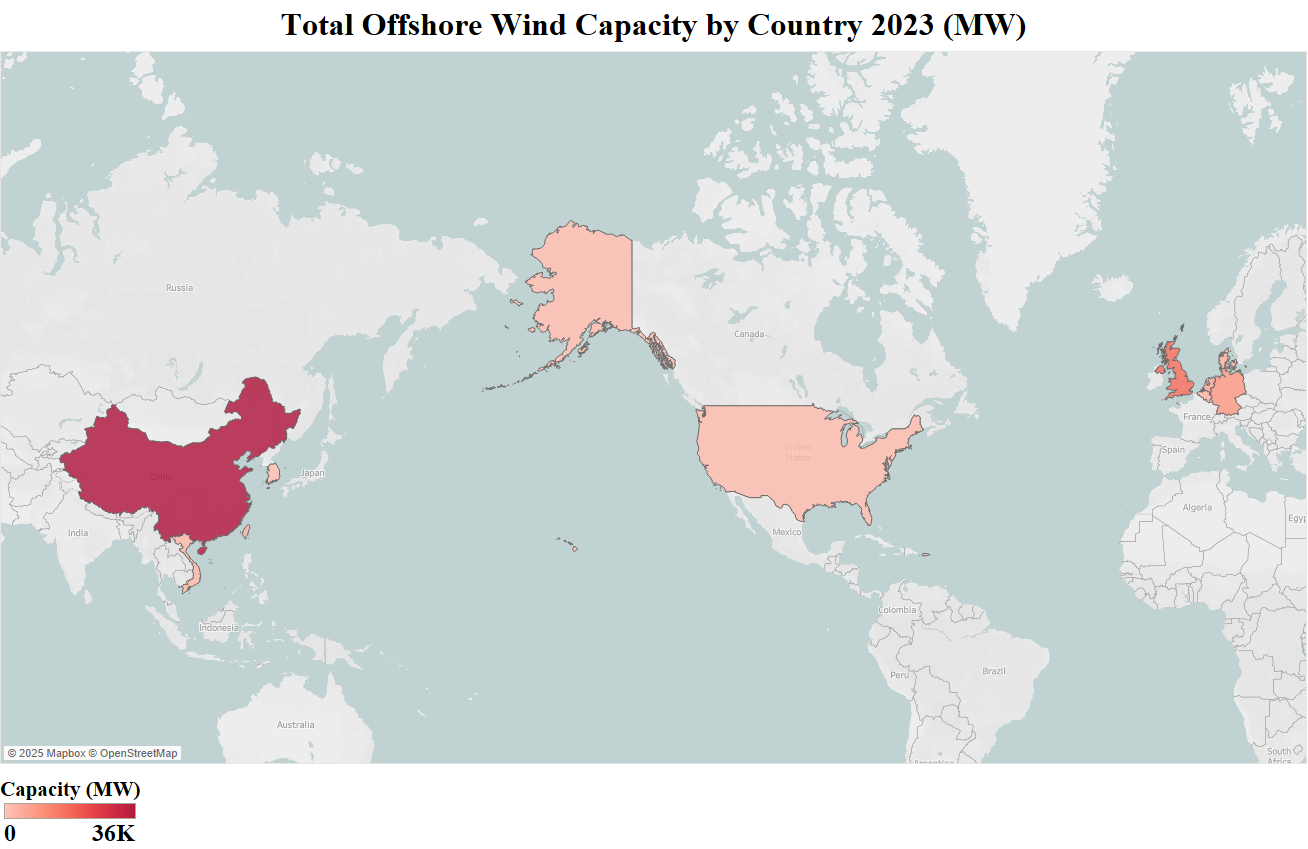
\includegraphics[width=3.2in]{Figures/singh1.png}}
\caption{Capacity of OWF Constructed as of 2023 According to DOE \cite{musial2023offshore}.}
\label{map}
\end{figure}

\begin{figure}[t]
\centerline{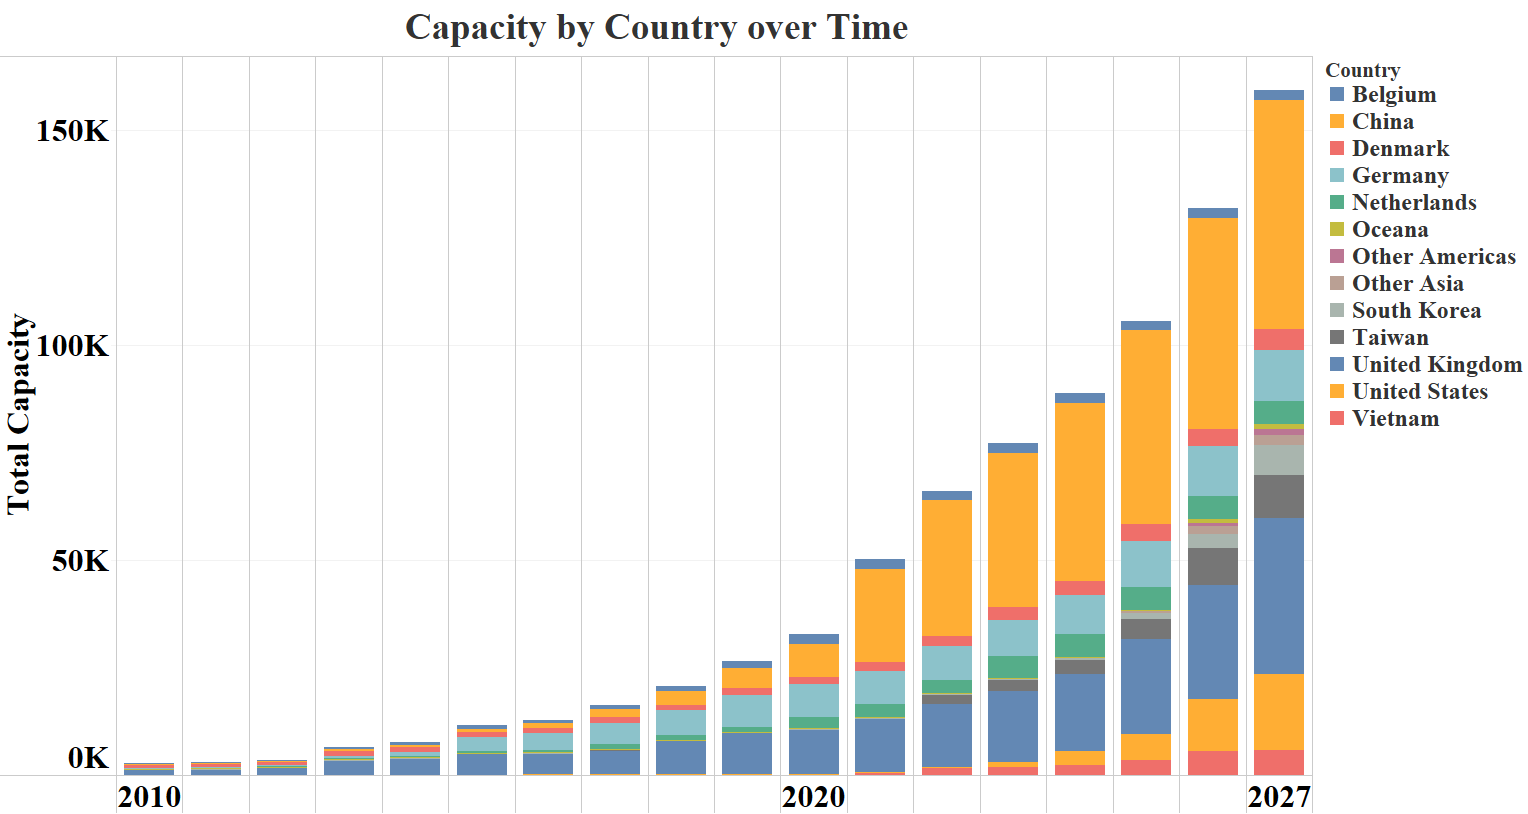
\includegraphics[width=3in]{Figures/singh2.png }}
\caption{Total Capacity (MW) of OWF by Country by Year According to DOE.}
\label{stacked bar}
\end{figure}


\begin{table*}[htbp]
\renewcommand{\arrayrulewidth}{1.1pt} % Ensures uniform border thickness
\renewcommand{\arraystretch}{1.2} % Increases row height for better readability
\centering
\caption{Wind Farms over 500 MW in Operation Worldwide}
\label{WindFarms}

\begin{tabular}{|p{2.1cm}|p{0.85cm}|p{1.3cm}<{\centering\arraybackslash}|p{1.25cm}<{\centering\arraybackslash}|p{1.2cm}<{\centering\arraybackslash}|p{1.6cm}<{\centering\arraybackslash}|p{1.8cm}<{\centering\arraybackslash}|p{1.8cm}<{\centering\arraybackslash}|p{1.4cm}<{\centering\arraybackslash}|}  
\hline
\textbf{Project Name} & 
\textbf{Year} & 
\textbf{Power Rating (MW)} & 
\textbf{Type of System} & 
\textbf{Number of Turbines} & 
\textbf{Substation} & 
\textbf{Cable Length to Shore} & 
\textbf{Cable Details} & 
\textbf{Architecture} \\  
\hline  

\textbf{Beatrice} & 2019 & 588 & HVAC & 84 & - & 70 km & Two composite bundles (970 m and 1920 m) & Star \\  
\hline
\textbf{East Anglia} & 2020 & 714 & HVDC & 102 & 66 /220 kV & 87 km & Two transmission cables & - \\  
\hline
\textbf{Greater Gabbard} & 2012 & 504 & HVAC & 140 & 132/33 kV (Offshore) & 22.5 km & 3 phase 18/30(36) kV power core & - \\  
\hline
\textbf{Gwynt Y Mor} & 2015 & 576 & HVAC & 160 & Two 33 kV and 132 kV (Offshore) & 20 km & - & Star \\  
\hline
\textbf{Hornsea 2} & 2022 & 1300 & HVDC & 165 & - & 120 km & - & - \\  
\hline
\textbf{Hornsea 1} & 2019 & 1200 & HVDC & 174 & - & 120 km & - & - \\  
\hline
\textbf{London Array} & 2013 & 630 & HVAC & 175 & Two 33 kV & 54 km & Three copper core conductors & Radial \\  
\hline
\textbf{Moray East} & 2022 & 950 & HVAC & 100 & Three (Offshore) & 22 km & - & Radial \\  
\hline
\textbf{Triton Knoll} & 2022 & 857 & HVAC & 90 & - & 57 km & 220 kV HVAC & - \\  
\hline
\textbf{Walney} & 2018 & 659 & HVAC & 87 & - & 44 km & - & Point-to-point \\  
\hline
\textbf{Kriegers Flak} & 2021 & 605 & HVDC & 72 & - & 44 km & - & MTDC \\  
\hline
\textbf{Gemini} & 2017 & 600 & HVAC & 130 & Two offshore high voltage substations & 110 km & 230 kV alternating current & Star \\  
\hline
\textbf{Guangdong Jieyang Shenquan 2} & 2023 & 502 & HVAC & 50 & 220 kV offshore booster station & 22 km & 220 kV export cables \& 66 kV inter-array cables & - \\  
\hline
\textbf{Guangdong Shanwei Jiazi 1} & 2022 & 503.1 & HVAC & 78 & One 500 kV & 25 km & - & - \\  
\hline
\textbf{Guangdong Yangjiang Qingzhou Iii} & 2022 & 500.6 & HVAC & 30 & - & 142 km & 75 km of 220 kV \& 142 km of 35 kV XLPE subsea cables & - \\  
\hline
\textbf{Guangdong Zhanjiang Xuwen} & 2020 & 608.65 & HVAC & 25 & - & 27.5 km & - & - \\  
\hline
\textbf{Shandong Bozhong A} & 2022 & 501 & HVAC & 60 & - & 20 km & - & Star \\  
\hline
\textbf{Yunlin} & 2021 & 640 & HVAC & 80 & Two substations (4 x 66/161-kV each) & 270 km & - & - \\  
\hline  

\end{tabular}

\end{table*}


As HVDC-based OWFs become increasingly pivotal in the global energy landscape, it becomes increasingly crucial to optimize their performance, reliability, and cost-effectiveness. Achieving this optimization requires a comprehensive understanding of key factors, including a technical and economic analysis of the system. This review seeks to explore these critical elements in detail, emphasizing their significance within the Offshore Wind Energy (OWE) sector. 

The economic viability of HVDC systems for OWFs is a pivotal aspect of feasibility analysis \cite{jiang2022tech}. A comprehensive economic evaluation, including factors such as initial investment, operational expenses, maintenance costs, and lifecycle assessments, is crucial to balancing technological advancements with financial feasibility. These economic considerations are intrinsically linked to technical decisions, as both impact the overall cost-effectiveness and reliability of the system.

The choice of connection topology exemplifies this interdependence. Configurations such as point-to-point, multiterminal, All-DC or hybrid systems significantly influence power collection and transmission efficiency, stability, and loss mitigation \cite{elahidoost2024stability, paul2022novel}. 
Each topology comes with distinct economic and technical trade-offs, affecting infrastructure costs, power flow control, and grid stability - key components in optimizing both performance and financial returns. Converter design is another keystone of HVDC systems that directly affects their efficiency, reliability, and adaptability to offshore environments. The selection between Voltage Source Converters (VSCs), Line-Commutated Converters (LCCs), and DC-DC converters carries substantial economic and technical implications \cite{korompili2016review, inamdar2018converters}. These converters determine the scalability and flexibility of the system, influencing not only the upfront costs but also the operational efficiency and maintenance requirements.

Technical modeling further bridges economic and technical analysis \cite{abedin2021dynamic, xia2023operation}. Accurate simulations, control strategies, and performance models optimize system design and operational reliability while enabling cost-effective planning. These models are essential to predict dynamic behaviors, minimize transmission losses, and ensure seamless grid integration \cite{wang2022large}. By combining technical insights with economic evaluations, modeling ensures that HVDC OWFs deliver sustainable and financially viable energy solutions. This interconnected approach underscores the need for holistic analysis, where economic and technical factors are jointly considered to maximize the efficiency, reliability, and cost-effectiveness of HVDC systems for OWFs.

Table \ref{research_paper} offers a comprehensive comparison of various research papers and evaluates their contributions in these four main dimensions to the best of the author's knowledge. The table provides a clear overview of the focus areas addressed in the existing literature, highlighting both strengths and gaps. 
Recent studies such as \cite{inamdar2018converters, li2021review, yu2024dru, hk2024review} review and compare various power converter architectures used in OWF integration. For example, \cite{inamdar2018converters} discusses converter topologies in HVDC systems for OWFs and provides a detailed analysis of the Modular Multilevel Converter (MMC) and its operational states. 

Similarly, \cite{li2021review} offers a comprehensive review of HVDC converter architectures used in both research and real-world OWF projects, exploring how advanced HVDC topologies can overcome offshore challenges by improving efficiency, reducing converter size and weight, and enhancing reliability. In \cite{yu2024dru}, a comparison of Diode Rectifier Unit (DRU)-based HVDC with other HVDC systems is presented, focusing on control, initialization solutions and fault management, along with future research directions. \cite{hk2024review} evaluates Multilevel Converters (MLCs) in VSC-based HVDC systems, highlighting their potential to improve efficiency, performance, and reliability for OWF integration.

In another key study, \cite{xu2023eight} compares eight offshore wind power transmission schemes based on economic viability, reliability, and technological maturity, recommending accelerated development of HVDC and Low Frequency AC (LFAC) technologies for grid-following and grid-forming OWFs. \cite{li2020review} further provides an extensive review of HVDC transmission topologies, converter technologies, and control strategies for OWFs, highlighting their role in enhancing system reliability and fault ride-through capabilities.

Several papers focus on the economic analysis of OWF integration technologies. For instance, \cite{hardy2019techno, kucuksari2019impact, fernandez2019offshore, xiang2021comparison} present detailed economic analyses that explore the financial viability and technical performance of HVAC, HVDC, and LFAC technologies, emphasizing factors such as Levelized Cost of Energy (LCOE), cost optimization, and transmission distance. These analyses are crucial for strategic decision-making in selecting the most suitable technologies for OWF collection and grid integration. Similarly, \cite{houghton2016offshore, stamatiou2010techno, bresesti2007hvdc} provide valuable insights into the economic benefits of different HVDC connection strategies for OWFs, promoting efficient and cost-effective offshore transmission solutions.

In \cite{sun2021reliability}, the author evaluates four different offshore wind power DC collection topologies using the Universal Generating Function technique, offering a reliable and economic assessment from both technical and economical perspectives. Additionally, \cite{meng2021comparative} conducts a comparative economic analysis of LFAC, HVDC, and HVAC systems, determining the most cost-effective transmission solution based on capital costs, converter topologies, and transmission capacities. \cite{saraswati2022offshore} compares Medium Voltage DC (MVDC) and HVAC systems for different OWF topologies through an integrated techno-economic analysis, focusing on energy efficiency, CAPEX, OPEX, and LCOE, using case studies to emphasize the role of connection topologies in improving OWF reliability and economics.

Further expanding on the economic and technical dimensions, \cite{alassi2019hvdc} offers insights for stakeholders on the trajectory of technology development and market dynamics by comparing HVDC and HVAC systems across complex technical and economic factors through a practical case study. Similarly, \cite{yang2022critical} comprehensively evaluates various grid connection technologies for large OWFs, considering transmission systems, fault ride-through strategies, and economic feasibility. Focusing on collection, \cite{lakshmanan2021electrical} reviews OWF electrical collection systems, categorizing them into AC, DC, and LFAC systems, with a focus on cost reduction, improved energy efficiency, and enhanced reliability. This work highlights the importance of DC-DC converters and novel protection systems, while underscoring the potential of LFAC and DC systems to reduce platform sizes and optimize system design. However, the paper could benefit from deeper insights into the technical modeling.

On the other hand, \cite{deng2023review} provide a comprehensive review of OWF HVDC systems, focusing on advanced converter topologies like hybrid MMC, Alternate Arm Converters (AAC), and Diode Rectifiers (DR). The work emphasizes key operational aspects such as control strategies, stability analysis, and fault protection, with a particular focus on future research directions involving system evaluation methods and the role of advanced semiconductor materials for greater efficiency. However, a more detailed economic analysis could further enhance the paper's insights.

Despite the existing body of research, a notable gap persists in the form of a lack of studies that comprehensively address all four critical dimensions; economic analysis, connection topology, converter design, and technical modeling in a single review. This paper aims to bridge that gap by providing the examination of these key dimensions, offering a more integrated understanding of their interactions and mutual influences. By adopting this holistic approach, the paper seeks to guide the effective optimization and implementation of HVDC technology in OWE projects.


\subsection{\textbf{Contribution of the paper}}

This paper reviews the existing research, innovations, and methodologies relevant to the economical analysis, connection\\ topology, converter design, and technical modeling within the realm of HVDC OWFs.
 %It is crucial for optimizing design, predicting operational behaviors, and facilitating seamless onshore grid integration.
 \begin{itemize}
\item \textbf{Economic Analysis:} This article examines the economic aspects of HVAC vs. HVDC architectures emphasizing cost factors, reliability and discounting to bridge economic and technical perspectives, identify gaps, and improve techno-economic analysis for offshore wind integration. 
\item \textbf{Connection Architectures:} The paper evaluates collection grid configurations for HVDC transmission including emerging architectures. 
The anlysis consider reliability, control, scalability, and cost implications to economic and technical performance.
\item \textbf{Converter Designs:} It examines various converter topologies, including Voltage Source Converters (VSCs), Line Commutated Converters (LCCs), and DC-DC converters, analyzing their efficiency, reliability, and adaptability for offshore wind farm integration across both collection and transmission systems. 
\item \textbf{Technical Modeling:} Simulation and modeling techniques are reviewed to optimize performance, balance computational efficiency, and support decision-making by predicting operational behaviors and system reliability for OFW system as a whole. \end{itemize}
By analyzing these multifaceted parameters, this review aims to provide a comprehensive framework that aids in informed decision-making and fosters the advancement of sustainable and economically viable OWE systems. 

 \subsection{\textbf{Organization of the paper}}
 The rest of the paper is organized as follows: Section II begins with a comprehensive economic analysis, focusing on the costs associated with HVDC and HVAC connections and economic considerations for reliability. 
 Section III delves into OWF connection architectures, thoroughly examining collection and transmission architectures. 
 It also includes a techno-economic analysis for both collection and transmission architectures, followed by a discussion of grid connection challenges. 
 Section IV explores power converter topologies, addressing both AC-DC and DC-DC converters and their suitability for HVDC based OWE collection and transmission. 
 Section V focuses on modeling techniques, highlighting the challenges in OWF modeling, the trade-offs between dynamics and efficiency, and the use of analytical approaches in both time-domain and frequency-domain analyses.
 This section also identifies key research gaps and areas for further exploration. 
 Section VI covers ongoing research and the future scope of OWF technologies, while Section VII provides the paper's conclusions, summarizing the key findings and insights.


\begin{table}[htbp]
\caption{Summary of Recent Review Articles}
\label{research_paper}
\renewcommand{\arrayrulewidth}{1.1pt} % Fixed border thickness
\renewcommand{\arraystretch}{1.1} % Adjust row height
\centering
\small

\begin{tabular}{|m{0.6cm}<{\centering}|m{1.2cm}<{\centering}|m{1.4cm}<{\centering}|m{1.22cm}<{\centering}|m{1.4cm}<{\centering}|}
\hline
\textbf{Ref} & 
\textbf{Converter Design} & 
\shortstack{\textbf{Connection}\\ \textbf{Topology}} & 
\textbf{Technical Modeling} & 
\textbf{Economic Analysis} \\ 
\hline

\cite{inamdar2018converters} & \cmark & \xmark & \xmark & \xmark \\ \hline
\cite{li2021review} & \cmark & \xmark & \xmark & \xmark \\ \hline
\cite{yu2024dru} & \cmark & \xmark & \xmark & \xmark \\ \hline
\cite{hk2024review} & \cmark & \xmark & \xmark & \xmark \\ \hline
\cite{xu2023eight} & \xmark & \cmark & \xmark & \xmark \\ \hline
\cite{li2020review} & \cmark & \cmark & \xmark & \xmark \\ \hline
\cite{hardy2019techno} & \xmark & \xmark & \xmark & \cmark \\ \hline
\cite{kucuksari2019impact} & \xmark & \xmark & \xmark & \cmark \\ \hline
\cite{fernandez2019offshore} & \xmark & \xmark & \xmark & \cmark \\ \hline
\cite{xiang2021comparison} & \xmark & \xmark & \xmark & \cmark \\ \hline
\cite{houghton2016offshore} & \xmark & \cmark & \xmark & \cmark \\ \hline
\cite{stamatiou2010techno} & \xmark & \cmark & \xmark & \cmark \\ \hline
\cite{bresesti2007hvdc} & \xmark & \cmark & \xmark & \cmark \\ \hline
\cite{sun2021reliability} & \xmark & \cmark & \xmark & \cmark \\ \hline
\cite{meng2021comparative} & \cmark & \xmark & \xmark & \cmark \\ \hline
\cite{saraswati2022offshore} & \xmark & \cmark & \xmark & \cmark \\ \hline
\cite{alassi2019hvdc} & \cmark & \cmark & \xmark & \cmark \\ \hline
\cite{yang2022critical} & \cmark & \cmark & \xmark & \cmark \\ \hline
\cite{deng2023review} & \cmark & \cmark & \cmark & \xmark \\ \hline
\cite{lakshmanan2021electrical} & \cmark & \cmark & \xmark & \cmark \\ \hline

\end{tabular}

\end{table}


\section{\textbf{Economic Analysis}}

\subsection{\textbf{Costs related to Connections}}

The cost structure for OWF differs significantly between HVDC and HVAC. Between the two, HVDC maintains the highest fixed cost but the lowest variable cost. The low variable costs are mainly due to the low line losses and the lower cost of lines \cite{hardy2019techno,assessing2018transmission}. The cost differential for one system over the other in OWF depends on the line length, the discount rate used, and the cost estimation technique.

The literature traditionally estimates the impacts of costs through discounted payback periods, LCOE, or Internal Rate of Return (IRR), with LCOE consistently being the most popular. Substantial prior work has examined the breakeven point between transmission technologies for OWF. Recent work places the breakeven point around 150 kilometers (93 miles) \cite{xiang2021comparison} for a 300 MW system; however, recent advances in HVDC converters have brought costs down significantly in the past decade. Due to these changes, estimates of the breakeven point have been halved since 2010 \cite{van2010economic}.

As a cost estimation method, LCOE represents the average minimum price at which electricity generated by a resource must be sold to make building the resource viable \cite{saraswati2022offshore}. LCOE provides the same project selections as net present value and focuses on the economic viability from the producer's perspective. LCOE can be calculated by dividing the discounted sum of investment expenditures $I_t$, operations expenditures $M_t$, and fuel expenditures $F_t$ by the discounted sum of electricity generated $E_t$.


\begin{align}
LCOE &= \frac{
\sum_{t=1}^{T} \frac{I_t + M_t + F_t}{(1 + r)^t}
}{
\sum_{t=1}^{T} \frac{E_t}{(1 + r)^t}
}
\end{align}


\begin{figure}[htbp]
\centerline{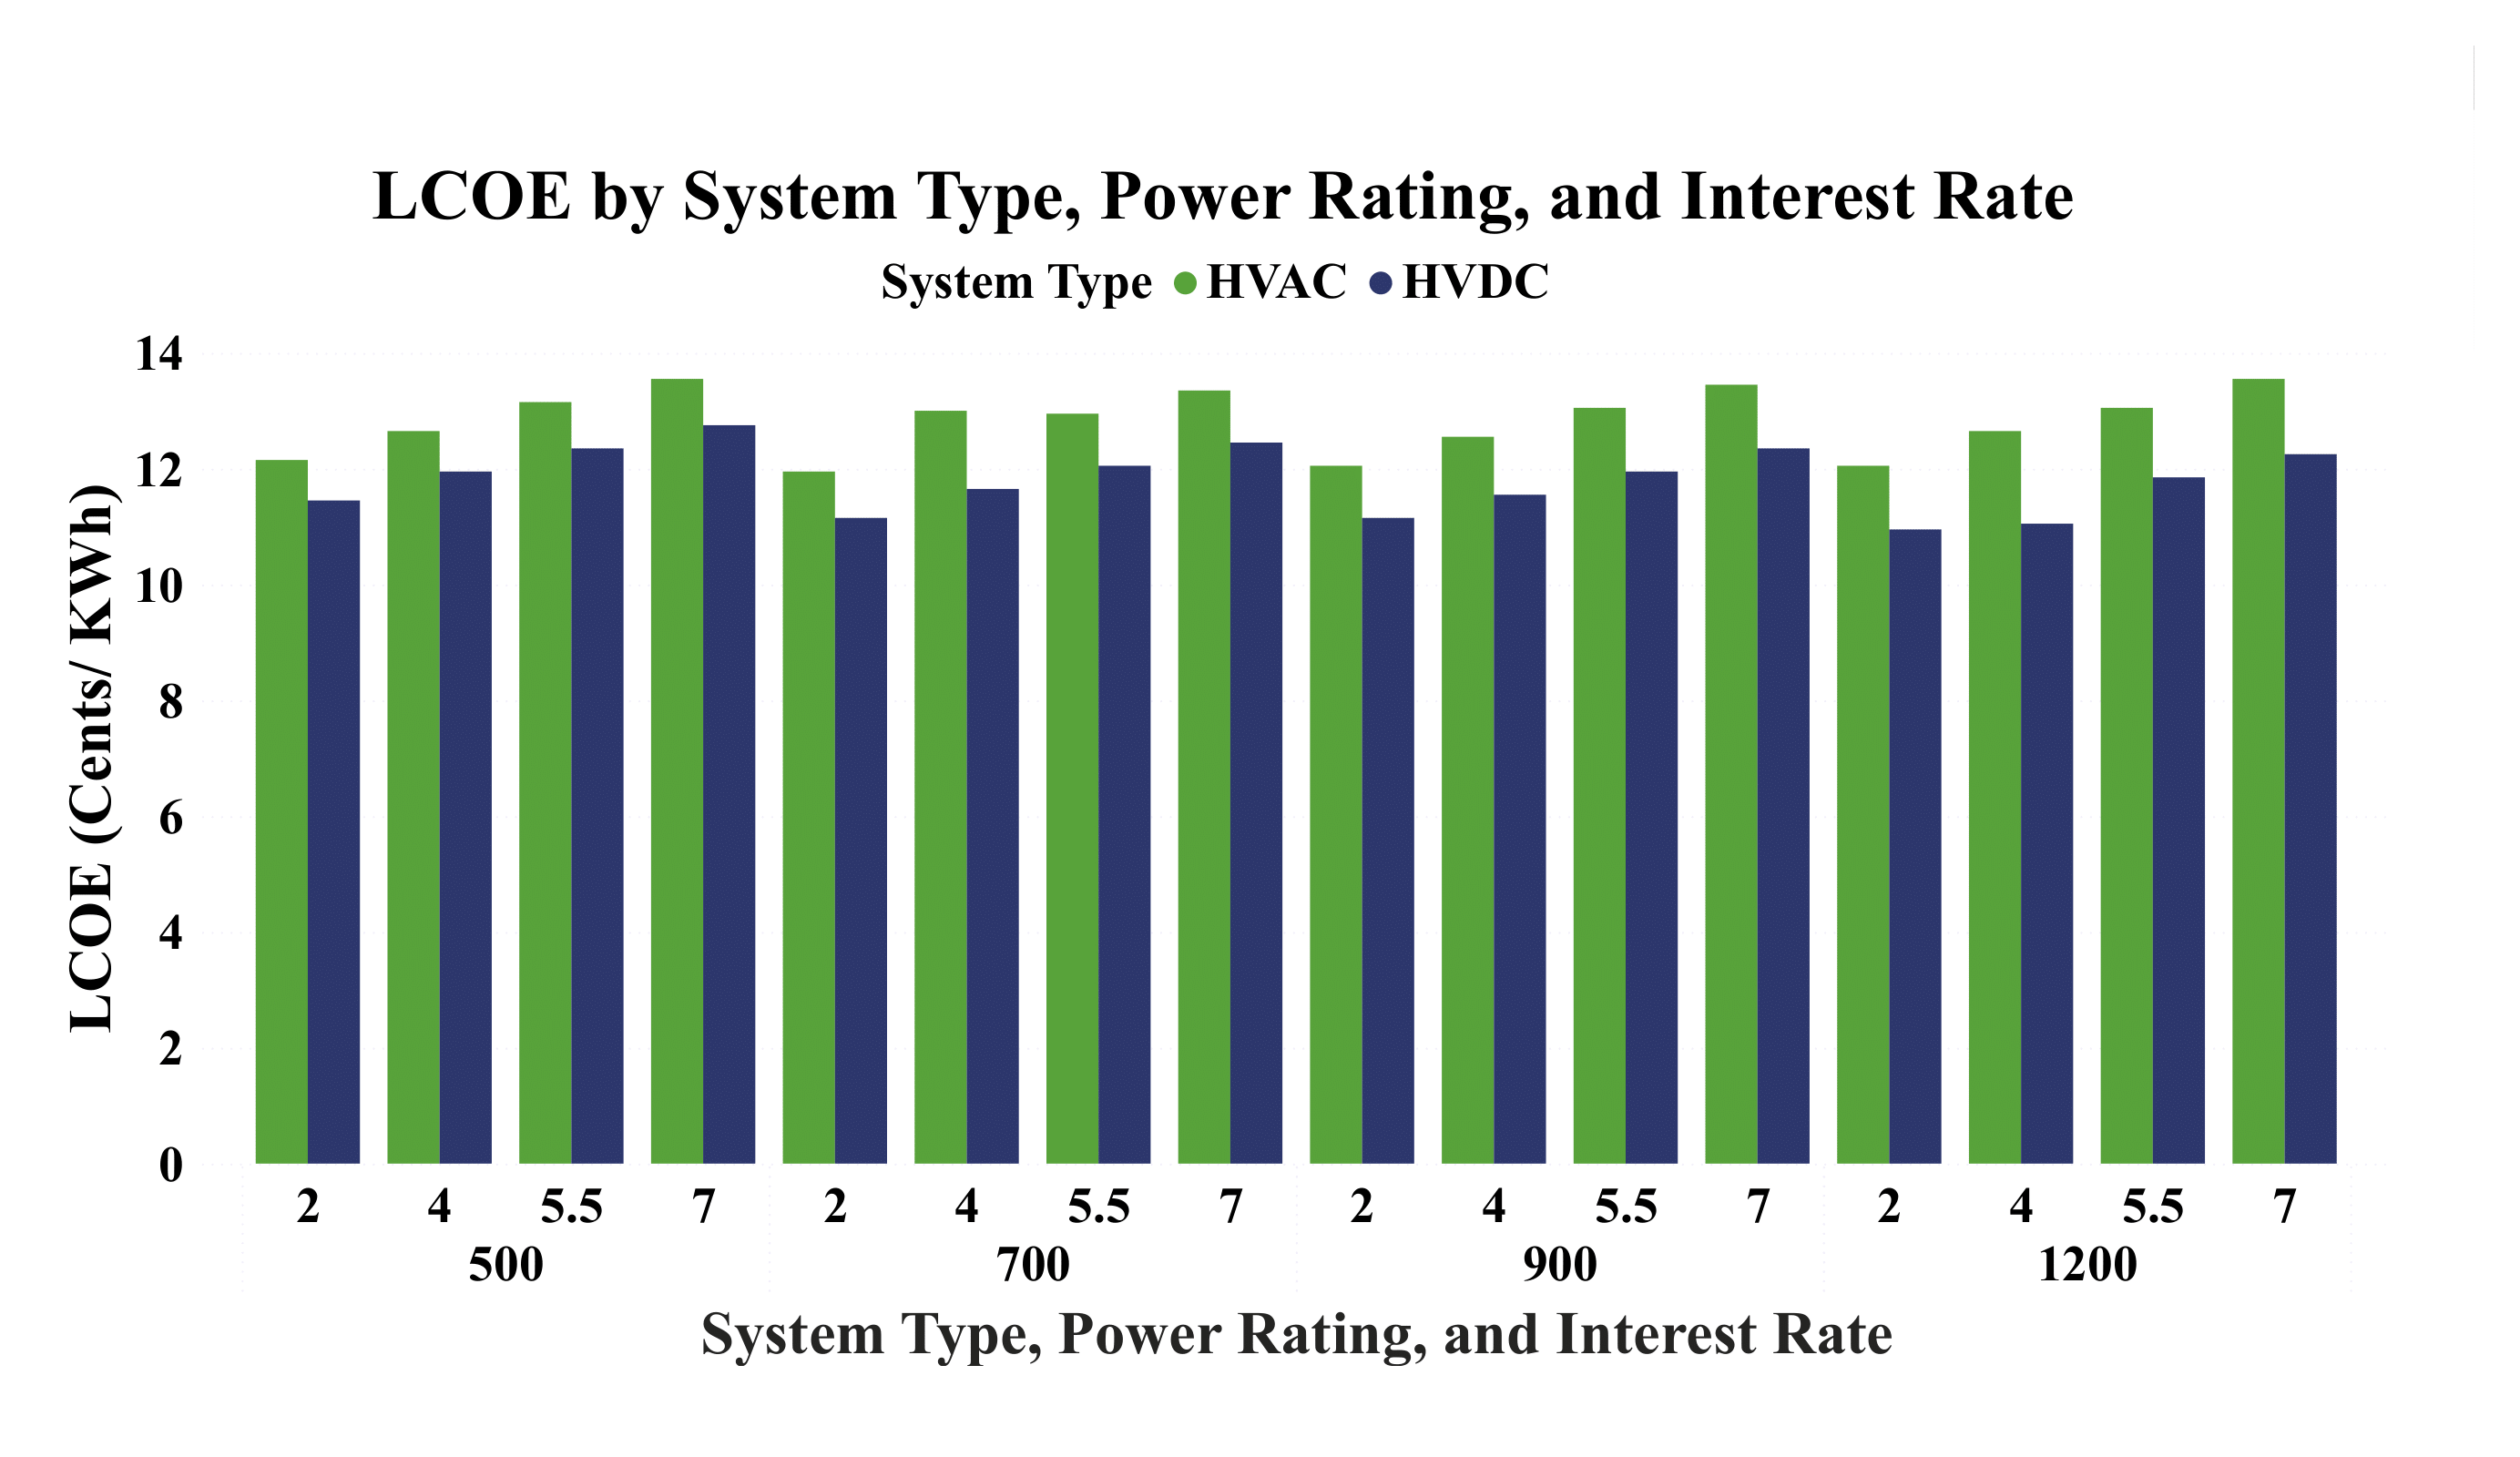
\includegraphics[scale=.25]{Figures/singh3.png}}
\caption{LCOE for Different System Types, Power Ratings, and Interest Rates.}
\label{interest rates Power Rating}
\end{figure}

Fig. \ref{interest rates Power Rating} shows the LCOE for HVDC and HVAC for power ratings at different baseline interest rates. To create the figure, the CREST LCOE calculator from the National Renewable Energy Laboratory (NREL) \cite{gifford2013crest} was used in conjunction with the estimates for the cost of the system from Table \ref{System cost} based on \cite{meng2021comparative}.

The baseline interest rate used to create Fig. \ref{interest rates Power Rating} is the interest rate for construction financing. The interest rates for reserves and long-term debt were adjusted based on this baseline interest rate. The costs related to capital that vary with the size of the wind farm were adjusted for larger OWFs. The HVAC system capacity factor was adjusted to a value of 3.3\% from the HVDC system's capacity factor to reflect line losses. A 150-kilometer distance was used to compare the systems. A standard retirement time of 20 years is used. These numbers are highly stylized and therefore should be treated as estimates with high variance and more value for comparison across system types than estimation of real-world LCOE.

Fig. \ref{interest rates} isolates the impact of increases in interest rates on system LCOE by holding the power rating constant at 1200 MW. Fig. \ref{LCOE by Distance} shows the LCOE by distance for the different types of system for a 1200 MW system at varying lengths from shore at 2\% interest. Note that the breakeven distance in terms of LCOE is shorter than the breakeven distance based only on capital costs (shown later in Fig. \ref{fig final}). This is because the LCOE calculation accounts for line losses $\sim 3.3\%$ lower for HVDC systems than for HVAC systems, which leads to higher discounted revenues over the system's lifecycle.


\begin{figure}[htbp]
\centerline{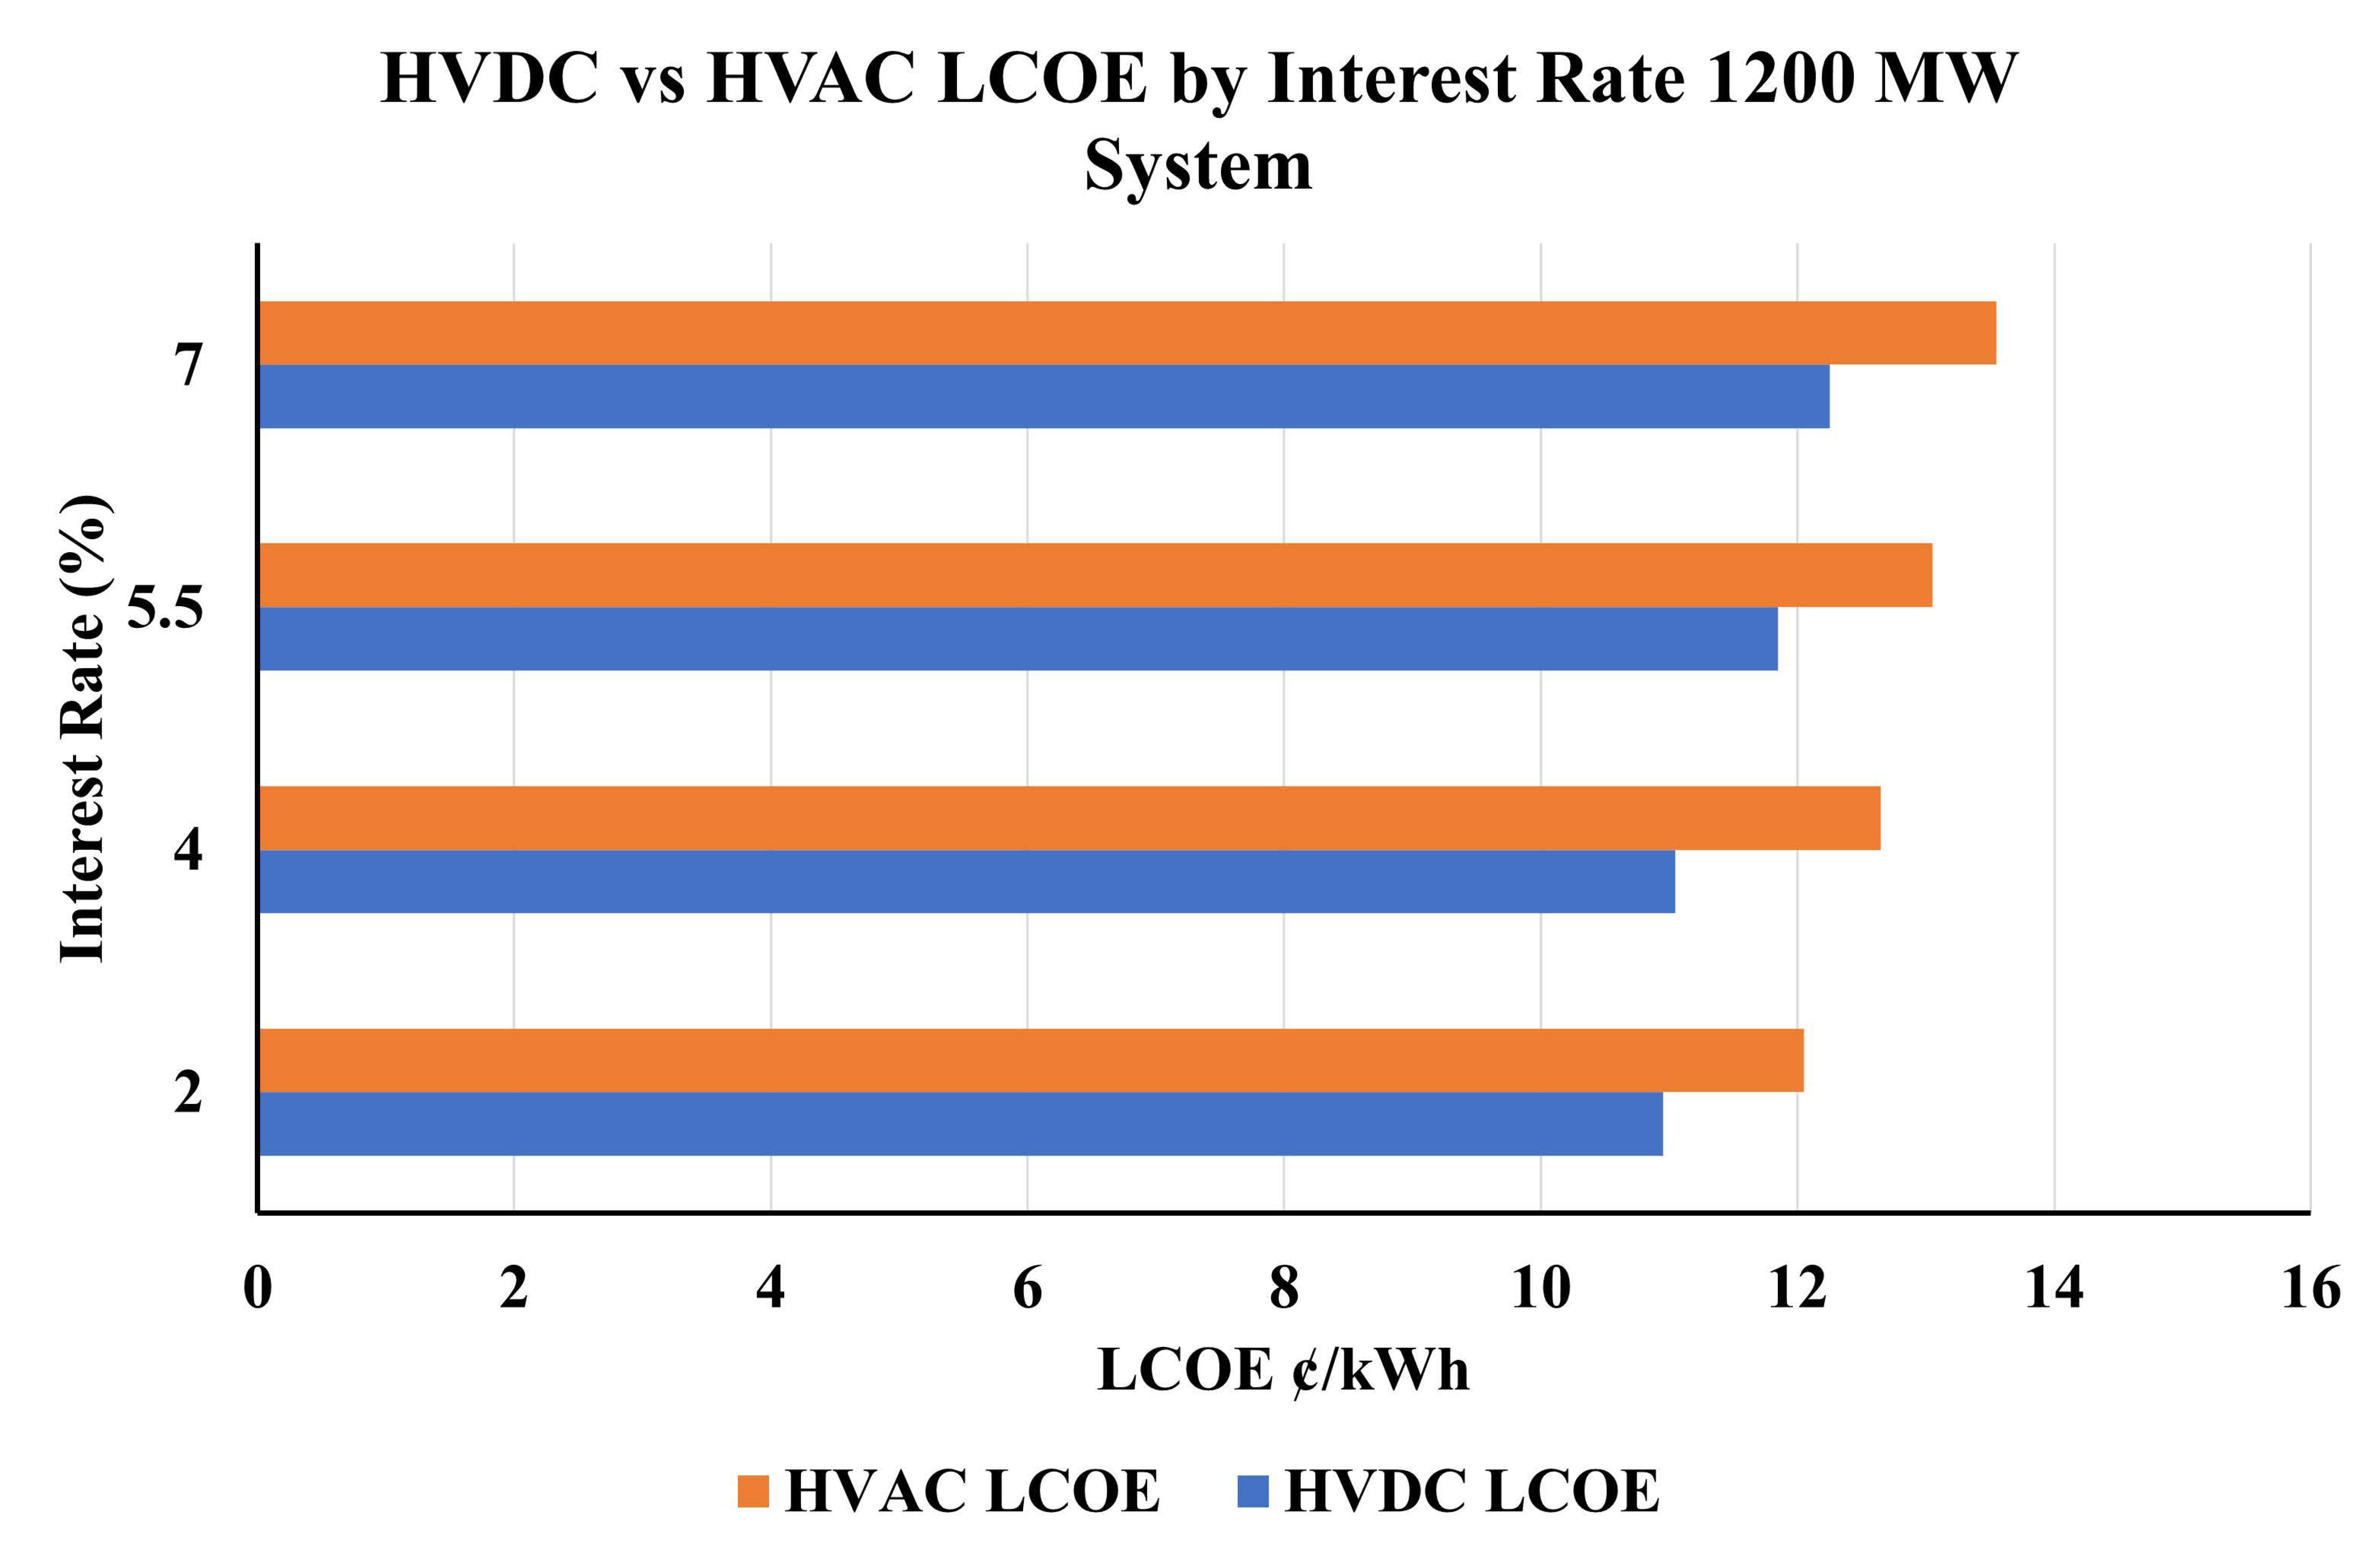
\includegraphics[scale=.35]{Figures/singh4.png}}
\caption{LCOE by Interest Rate and System Type for 1200 MW System.}
\label{interest rates}
\end{figure}

\begin{figure}[htbp]
\centerline{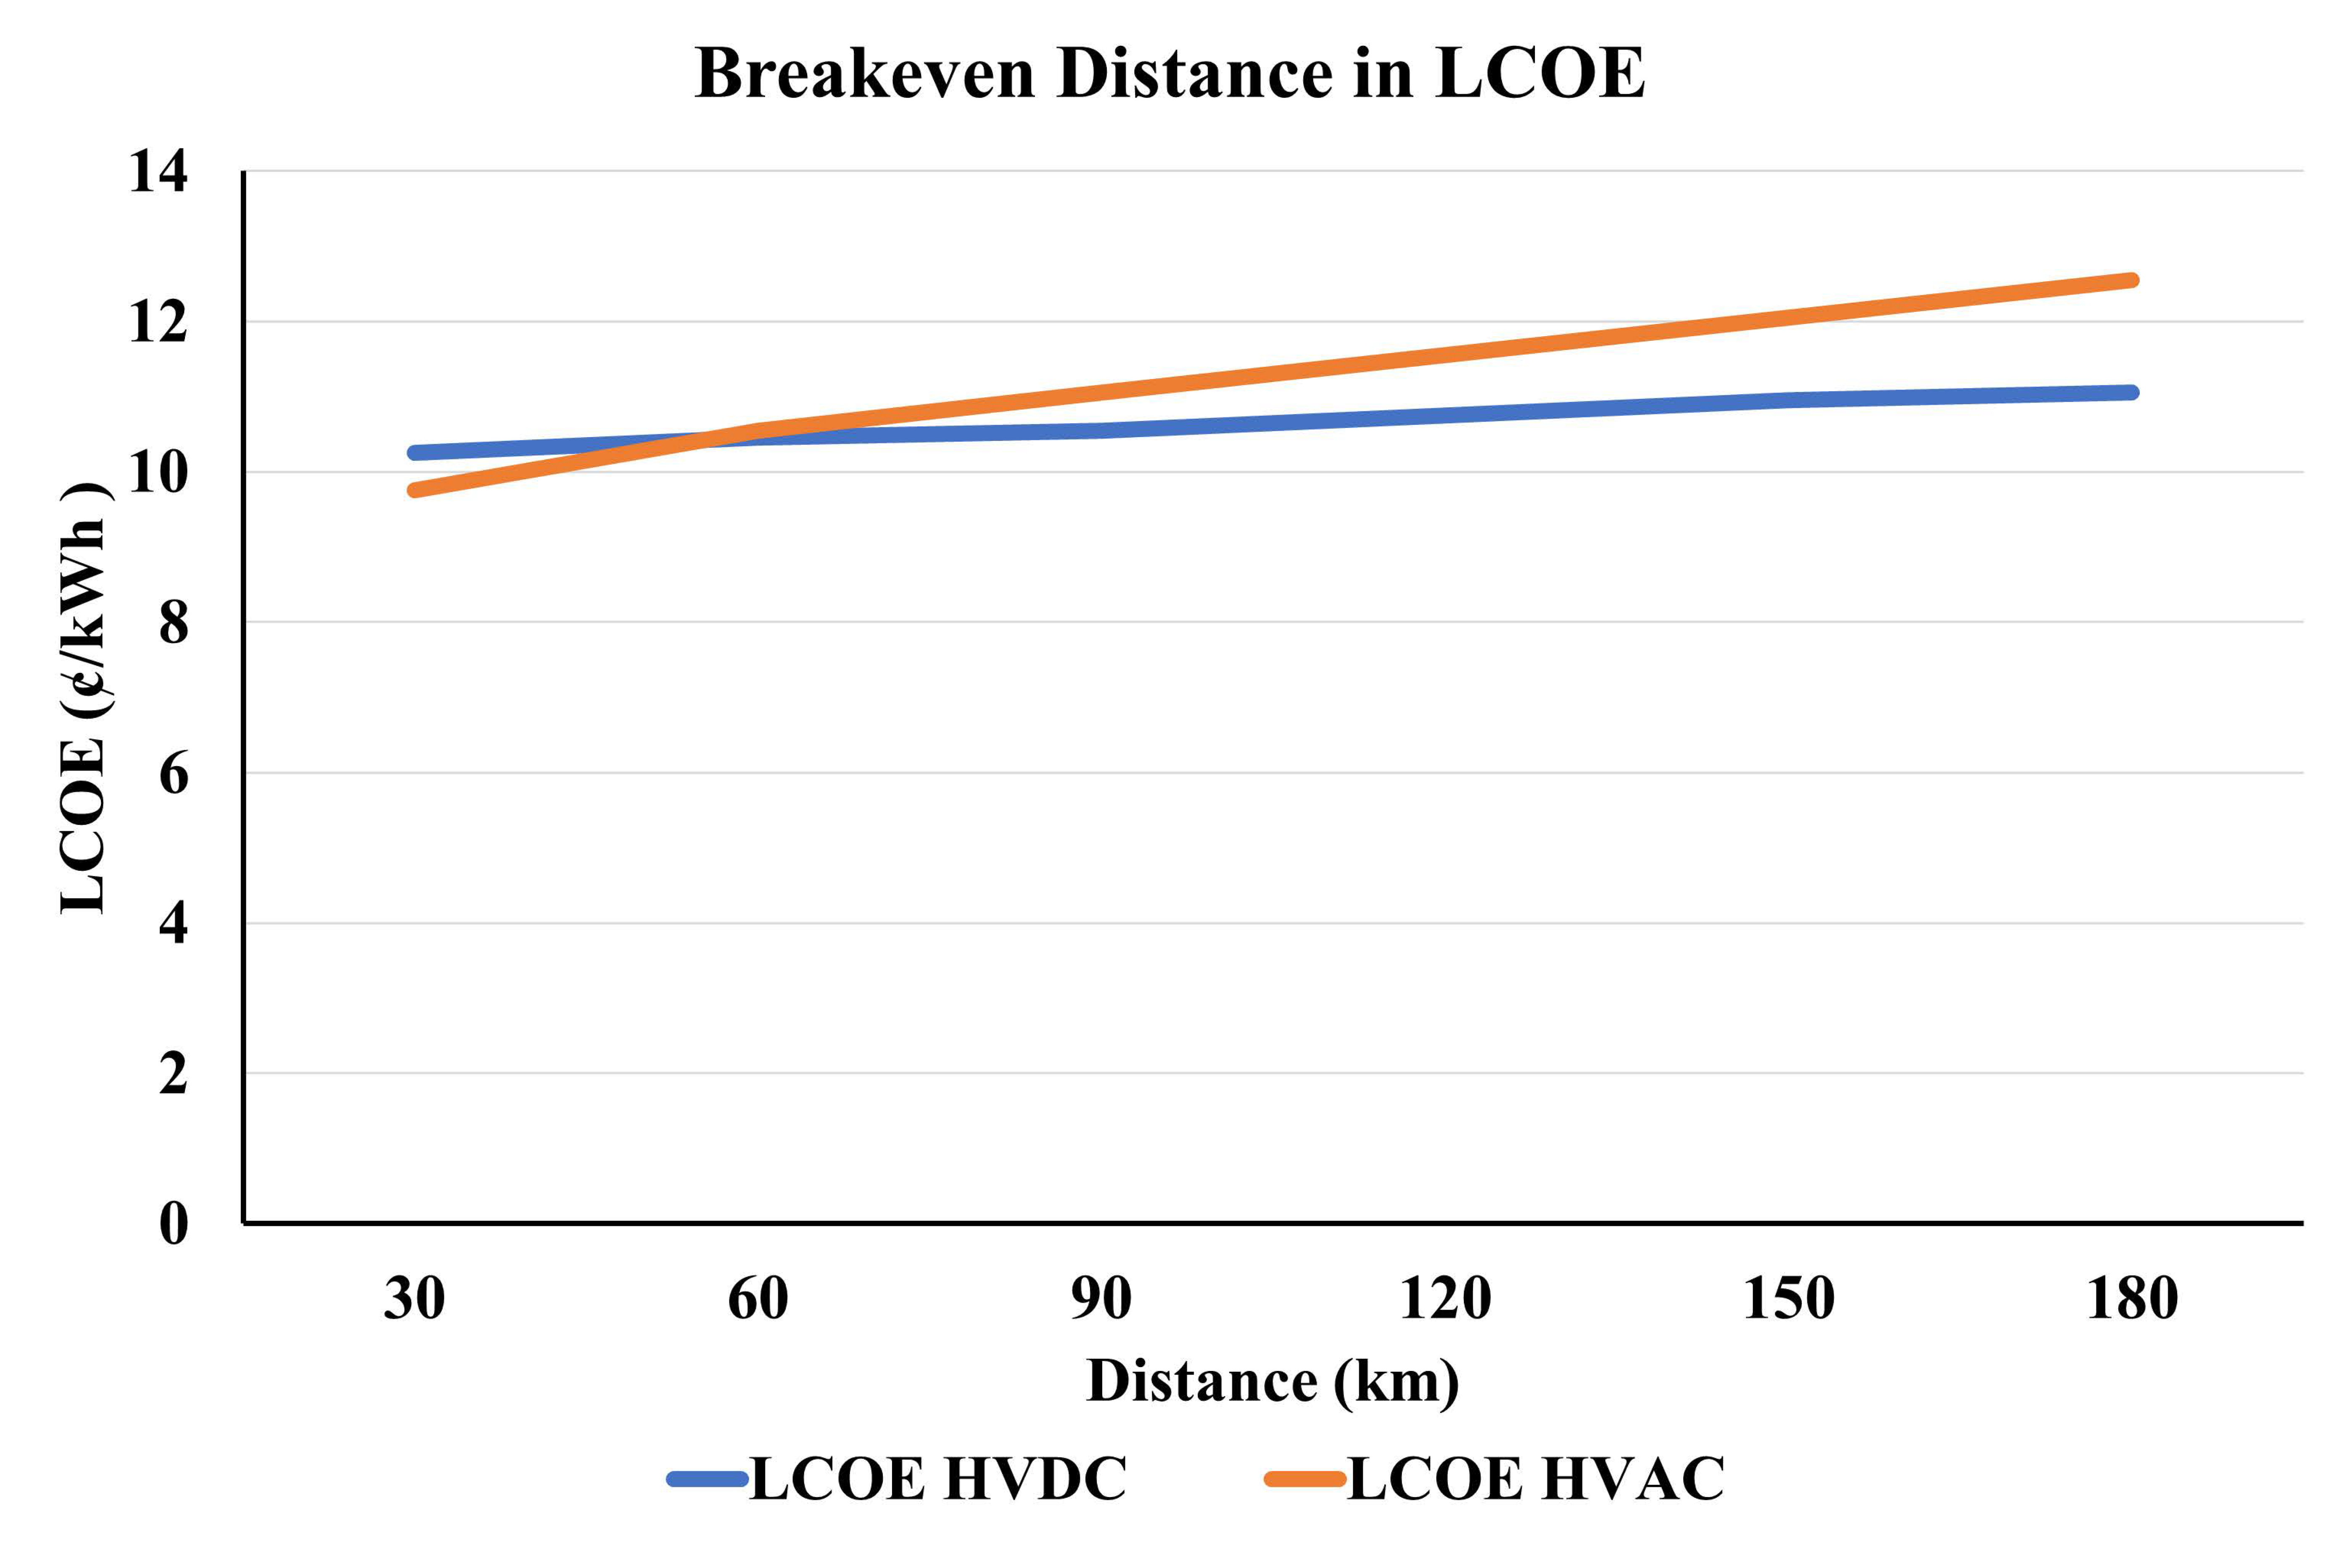
\includegraphics[scale=.35]{Figures/singh5.png}}
\caption{LCOE for Different System Types by Interest Rate for 1200 MW System.}
\label{LCOE by Distance}
\end{figure}

It should be noted that HVDC is more economical at all interest rates, but the difference between costs decreases as interest rates rise. This reduction in relative advantage is due to the increasing importance of fixed costs and the decreasing value of discounted future revenues as interest rates increase. Rising interest rates also cause a change in the most economical power rating as a result of the increase in the value of fixed costs and line losses.

The dramatically increased costs with higher interest rates show the impact of rising rates on OWF investment. The increase in LCOE helps explain the significant cancellation of OWF farms following increases in interest rates in recent years. At low interest rates of 2\%, 1200 MW HVDC systems are significantly cheaper than 1200 MW HVAC systems. This advantage becomes smaller as interest rates rise.

On the other side of a cost-benefit balance sheet, LACE (Levelized Avoided Cost of Energy) is a metric commonly used to complement LCOE. LACE provides the generator's value to the market as a whole or the increase in consumer surplus for the aggregate market \cite{kabeyi2023levelized}. When LACE exceeds LCOE, there is a net surplus and the resource will be net economically viable.

LCOE and LACE differ dramatically geographically, and NREL provides a map of the differences through the State and Local Planning for Energy (SLOPE) \cite{day2022state}. In 2020, the median offshore wind LCOE was 86 dollars per MWh, with the 2024 maximum at 126 dollars per MWh in Washington and a minimum of 72 on the Great Lakes in Ohio. In 2018, the most recent year on record, NREL put the highest LACE at 5 cents per KWh in Connecticut and the lowest at 1 cent per KWh in Wisconsin.

There are still substantive challenges to overcome before offshore wind becomes economically competitive at these rates. However, the median LCOE of offshore wind is projected to fall by 35\% by 2050, placing it below NREL's LCOE projections for combined cycles and making OWF competitive with most other energy sources. These estimates of LCOE are much higher than the current paper's estimates. Heterogeneity in system scale may help explain these differences, as the systems examined here are much larger and benefit from size compared to the systems currently in place in the United States.

An important area of future research is quantifying uncertainty related to LCOE estimates and finding ways to represent various future paths of revenues and costs. Although this research is in a stage that is developed for much of the techno-economic analysis literature, it is imperative in the case of offshore wind, where uncertainty about the learning curve and technological improvement leads to immense variability in LCOE estimates based on assumptions. Focusing on quantifying uncertainty would allow OWF research to follow the same path as other primary research into techno-economic analysis in other energy sources.

The metrics calculated within the literature often do not consider the impacts of the generators on other resources in the market, and an economical style analysis with an equilibrium model could yield an improved understanding of the fundamental values of changes in consumer welfare, and thus improve the estimation of LACE. The addition of electricity at peak load times proves particularly salient for consideration and can only be distinguished with a model that considers equilibrium effects. Also, because line losses increase at a quadratic rate with utilization, equilibrium impacts have outsized effects on costs.

Table \ref{tab:COst MIllions} shows how the cost estimate for the OWF components per megawatt varies depending on the chosen type of transmission system. High and low ends of ranges are based on quotes from papers within the literature \cite{kucuksari2019impact,meng2021comparative,xiang2021comparison,hardy2019techno,liu2023life}. 


\begin{table}[htbp]
\renewcommand{\arrayrulewidth}{1.1pt} % Border thickness
\renewcommand{\arraystretch}{1.2} % Row height for better readability
\arrayrulecolor{black}
\renewcommand{\tabcolsep}{5pt}
\small
\caption{Cost of Component by System for Set Size in Million Dollars}
\label{tab:COst MIllions}
\centering

\begin{tabular}{|p{3.6cm}<{\raggedright\arraybackslash}| p{1.7cm}<{\centering}| p{1.79cm}<{\centering}|}
\hline
\textbf{System} & \multicolumn{2}{l|}{\textbf{Cost of Component}} \\ 
\hhline{|>{\arrayrulecolor{white}}-|>{\arrayrulecolor{black}}--}
\textbf{Component} & {\bfseries HVDC (M\$)} & {\bfseries HVAC (M\$)} \\ 
\hline
\textbf{Substation} & 24-45 & 10-45 \\ 
\hline
\textbf{Cable} & 0.6/km & 1.5/km \\ 
\hline
\textbf{Offshore Platform} & 73.5 & 24 \\ 
\hline
\textbf{Onshore Platform} & 24 & 24 \\ 
\hline
\textbf{Cable Installation} & 215 & 215 \\ 
\hline
\textbf{Line Losses \% per 1000 km} & 0.035 & 0.067 \\ 
\hline
\multicolumn{3}{p{8cm}}{\textit{Note: Values are based on data provided in \cite{kucuksari2019impact,meng2021comparative,xiang2021comparison,hardy2019techno,liu2023life}}} \\ 
\hline
\end{tabular}
\end{table}




Beyond individual components, two other critical technical dimensions related to the cost-effectiveness of the two technologies are the size and the line length. As OWF has increased in size, and the cost compositions have changed both as a function of size and line length, breakeven analysis using these variables provides increasingly valuable information. Table \ref{System cost} compares the costs of the systems by line length and size in voltage rating using data from the literature \cite{meng2021comparative}.

\cite{meng2021comparative} considers three costs in a system: the Cost of the Onshore Platform (OPC), the Costs of the Offshore Platform and Plant (OPPC), and the cost of the cable $C_{Cable}$. The cost of the cable varies directly proportionately to the number of sets, the length of the line, and the price per kilometer. All cost estimates were taken from the appendix to \cite{meng2021comparative}. These costs differ by line length $l$ and system size $S_N$ according to \cite{meng2021comparative}.


\begin{table}[htbp]
\caption{Cost of System in Million Dollars by Size and Line Length} \label{System cost}
\renewcommand{\arrayrulewidth}{1.1pt} % Border thickness
\arrayrulecolor{black}
\renewcommand{\arraystretch}{1.2} % Row height
\small
\centering
\begin{tabular}{|
p{1.5cm}<{\centering}|
p{1.6cm}<{\centering}|
p{1.7cm}<{\centering}|
p{1.6cm}<{\centering}|}
\hline
\textbf{Power Rating} & \textbf{Line Length} & \multicolumn{2}{c|}{\textbf{System Cost}} \\
\hhline{|>{\arrayrulecolor{white}}-|
         |>{\arrayrulecolor{white}}-
         |>{\arrayrulecolor{black}}--|}
\textbf{(MW)} & \textbf{(km)} & {\bfseries HVDC (M\$)} & {\bfseries HVAC (M\$)} \\
\hline

\multirow{4}{*}{\textbf{300}}  & 30  & 142  & 54  \\
                                & 90  & 196  & 147 \\
                                & 150 & 248  & 232 \\
                                & 210 & 299  & 315 \\
\hline

\multirow{4}{*}{\textbf{500}}  & 30  & 226  & 94  \\
                                & 90  & 284  & 151 \\
                                & 150 & 342  & 267 \\
                                & 210 & 400  & 382 \\
\hline

\multirow{4}{*}{\textbf{700}}  & 30  & 370  & 125 \\
                                & 90  & 349  & 208 \\
                                & 150 & 421  & 487 \\
                                & 210 & 493  & 607 \\
\hline

\multirow{4}{*}{\textbf{900}}  & 30  & 398  & 204 \\
                                & 90  & 441  & 273 \\
                                & 150 & 527  & 485 \\
                                & 210 & 613  & 696 \\
\hline

\multirow{4}{*}{\textbf{1200}} & 30  & 538  & 251 \\
                                & 90  & 568  & 370 \\
                                & 150 & 662  & 660 \\
                                & 210 & 757  & 950 \\
\hline

\multicolumn{4}{l}{\textit{Note: Values are based on data provided in \cite{meng2021comparative}}} \\
\hline
\end{tabular}
\end{table}


\begin{table*}[htbp]
\caption{Economic Challenges to Offshore Wind Industry}
\renewcommand{\arrayrulewidth}{1.1pt}
\arrayrulecolor{black}
\renewcommand{\arraystretch}{1.3} % Adjust row height for better readability
\small
\centering
\label{economical challenge}

\begin{tabular}{|
p{2.8cm}<{\raggedright\arraybackslash} |
p{4.3cm} <{\raggedright\arraybackslash}|
p{5.3cm}<{\raggedright\arraybackslash} |
p{1.7cm}<{\raggedright\arraybackslash}|}
\hline
\multicolumn{2}{|l|}{\textbf{Main Challenge}} &
\textbf{Mitigation Strategy} &
\textbf{References} \\ \hline

\multicolumn{1}{|l|}{\textbf{Long-term Financing}}&
Capital Intensive &
\begin{tabular}[c]{@{}l@{}}
$-$ Subsidies for wind energy development \\
$-$ Renewable Portfolio Standards \\
$-$ Feed-in tariffs
\end{tabular} &
\cite{garcia2017analysis,heeter2019international} \\ \hhline{|>{\arrayrulecolor{white}}-|>{\arrayrulecolor{black}}---}  

\multicolumn{1}{|l|}{} &
Cost and Revenue Uncertainty &
\begin{tabular}[c]{@{}l@{}}
$-$ Contracts for Differences \\
$-$ Long-term electricity price modeling \\
$-$ Power purchase agreements \\
$-$ Inflation Adjustments
\end{tabular} &
\cite{welisch2020auctions,beiter2024enduring,jansen2022policy} \\ \hline

\multicolumn{1}{|l|}{} &
Low Revenues for Baseload Generators &
\begin{tabular}[c]{@{}l@{}}
$-$ Capacity market redesign \\
$-$ Convex hull pricing
\end{tabular} &
\cite{papalexopoulos2015modeling,mozdawar2022multiple,schiro2015convex} \\ \hhline{|>{\arrayrulecolor{white}}-|>{\arrayrulecolor{black}}---}  

\multicolumn{1}{|l|}{\multirow{-3}{*}{\textbf{Missing Money Problem}}} &
{Increased Ramping by Dispatchable Resources} &
\begin{tabular}[c]{@{}l@{}}
$-$ Improved cold start efficiency \\
$-$ Diversified portfolios \\ \hspace{8pt}(fossil and renewable)
\end{tabular} &
\cite{lamadrid2012ancillary,zou2021sustainable,kumar2019strategic} \\  \hhline{|>{\arrayrulecolor{white}}-|>{\arrayrulecolor{black}}---} 

\multicolumn{1}{|l|}{} &
Price Variability &
\begin{tabular}[c]{@{}l@{}}
$-$ Demand response \\
$-$ Energy storage systems (ESS) \\
$-$ Long-distance transmission
\end{tabular} &
\cite{wang2018optimization,botterud2024bridging,gonzales2022dynamic} \\ \hline

\multicolumn{1}{|l|}{} &
Waste of Wind Turbines &
\begin{tabular}[c]{@{}l@{}}
$-$ Turbine recycling \\
$-$ Reduced metal intensity
\end{tabular} &
\cite{chen2019recycling,jensen2018wind} \\ \hhline{|>{\arrayrulecolor{white}}-|>{\arrayrulecolor{black}}---}

\multicolumn{1}{|l|}{\multirow{-2}{*}{\textbf{Sustainable Supply Chain}}} &
Securing Metals for Turbine Production &
\begin{tabular}[c]{@{}l@{}}
$-$ Development of mineral sources \\
$-$ Supply chain transparency
\end{tabular} &
\cite{li2022future,nguyen2022electric} \\ \hline

\multicolumn{1}{|l|}{\textbf{Intermittency}} &
Non-dispatchability &
\begin{tabular}[c]{@{}l@{}}
$-$ Coordination with ESS \\
$-$ Black-start natural gas cooperation \\
$-$ Capacity market redesign
\end{tabular} &
\cite{gao2024techno,wang2018optimization,tarufelli2022capacity} \\ \hline

\multicolumn{1}{|l|}{\multirow{-1}{*}{\textbf{Concept to Industry}}} &
Initial Investments &
\begin{tabular}[c]{@{}l@{}}
$-$ Public-private partnerships \\
$-$ Loans via DOE programs \\
$-$ Government contracts \\\hspace{8pt} (e.g., Executive Order 14057)
\end{tabular} &
\cite{ExecutiveOrder2007,schwabe2017wind,de2012assessing} \\ \hhline{|>{\arrayrulecolor{white}}-|>{\arrayrulecolor{black}}---}

\multicolumn{1}{|l|}{} &
Workforce Development &
\begin{tabular}[c]{@{}l@{}}
$-$ Education funding \\
$-$ Project pipelines to retain knowledge
\end{tabular} &
\cite{stefek2022us,keyser2019wind,gowrisankaran2022policy} \\ \hline

\multicolumn{1}{|l|}{\textbf{Political Support}} &
Uncertain Technology Funding &
\begin{tabular}[c]{@{}l@{}}
$-$ Long-term funding guarantees \\
$-$ Resilience to leadership changes
\end{tabular} &
\cite{hu2018barriers,gowrisankaran2022policy} \\ \hline

\end{tabular}
\end{table*}



The values presented in Table \ref{tab:COst MIllions} and Table \ref{System cost} remain unadjusted for inflation to align with the original sources and ensure consistency. 
Since inflation impacts various cost components at different rates, applying adjustments would require assumptions that may not always be fully substantiated by available data. 
Recent studies \cite{fuchs2024cost, BNEF2023} highlight cost increases in offshore wind projects due to supply chain challenges and market dynamics since 2020, while strategic long-term planning has been recognized as a key factor in mitigating these costs. 
Additionally, \cite{EIA2015TEA} provides a structured approach for incorporating inflation adjustments into techno-economic analyses, offering a framework to enhance the accuracy and depth of cost evaluations.

The impact of interest rate risk on the cost of investment in OWF systems has yet to be considered as most papers assume the interest rate throughout life or do not consider line losses in breakeven analysis. However, the discount rate increases with rising interest rates, and the breakeven point between technologies changes, as shown above. Considering the impacts of different interest rates on the lowest-cost technology would allow for a more realistic estimation of the breakeven distance.

 Fig. \ref{Breakeven} below shows the breakeven distance using approximate cost data from \cite{meng2021comparative} to plot the breakeven point by system rating and is followed by Fig. \ref{fig final}. Fig. \ref{fig final} directly compares the approximated breakeven point by system rating. The breakeven point decreases uniformly because of economies of scale. The variable costs of cables increase substantially faster for HVDC than for HVAC.


\begin{figure}[htbp]
\centerline{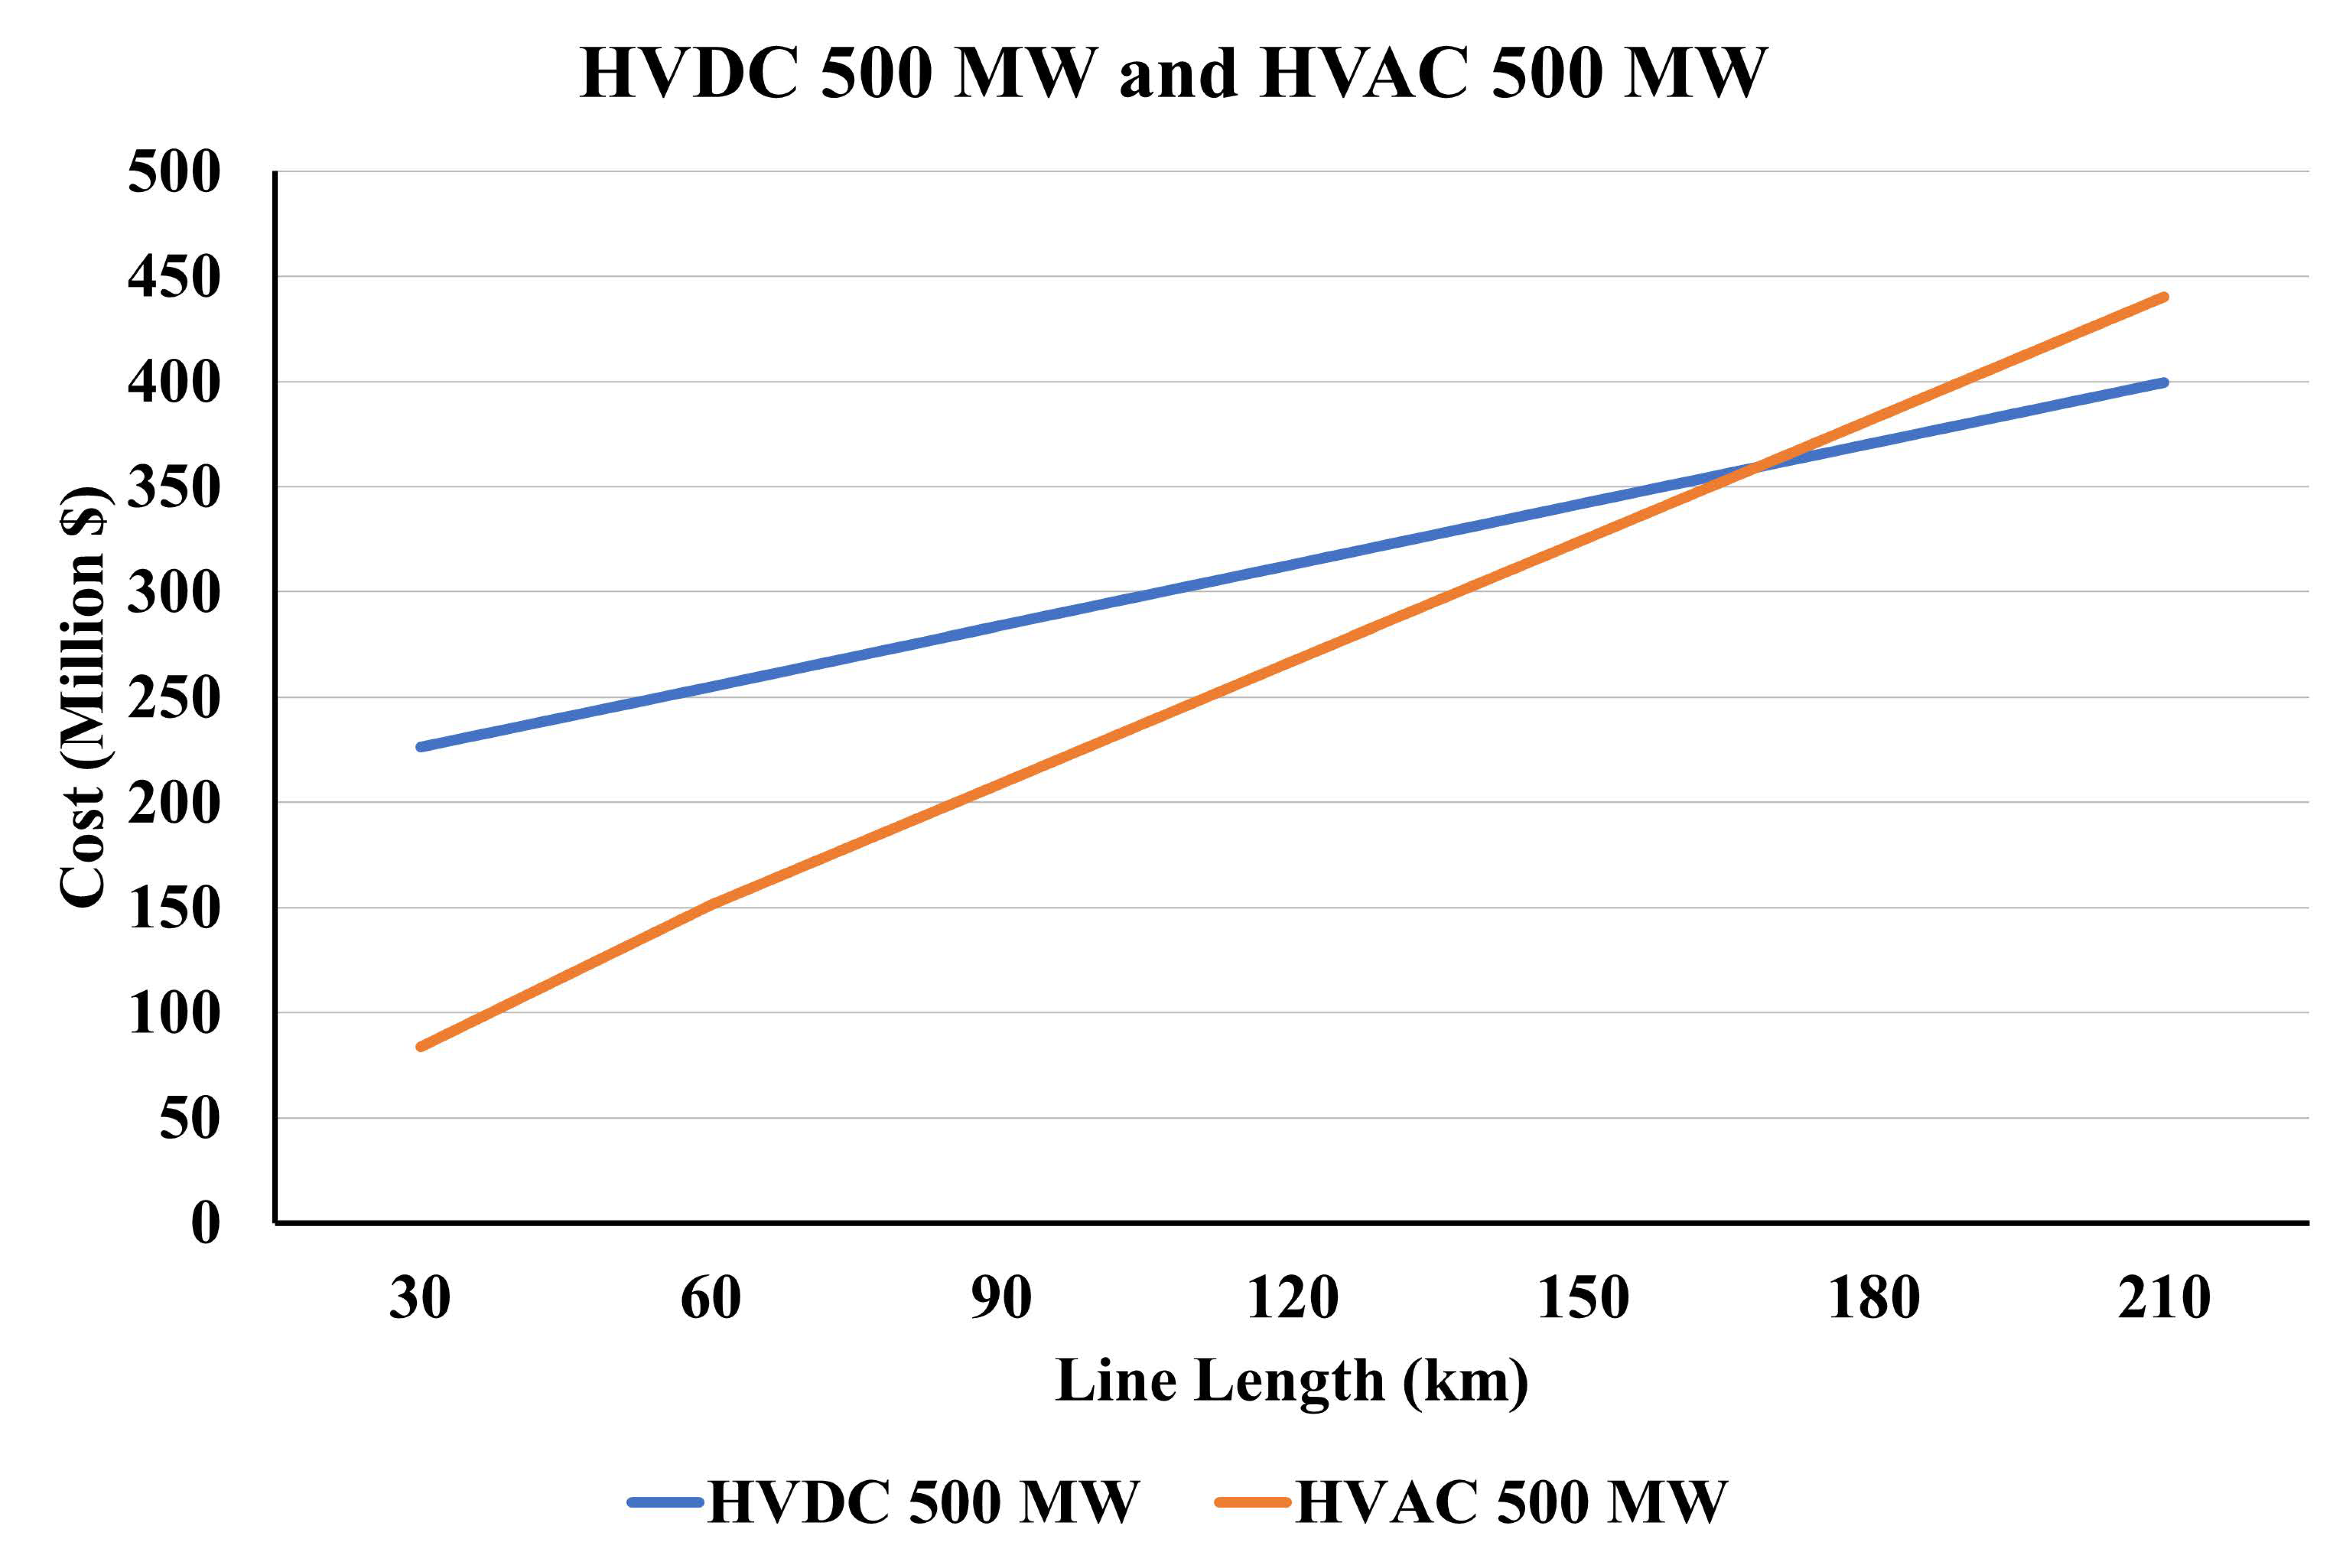
\includegraphics[scale=.35]{Figures/singh6.png}}
\caption{Breakeven Point for Systems of Differing Ratings without Considering Life Cycle Costs.}
\label{Breakeven}
\end{figure}


\begin{figure}[htbp]
\centerline{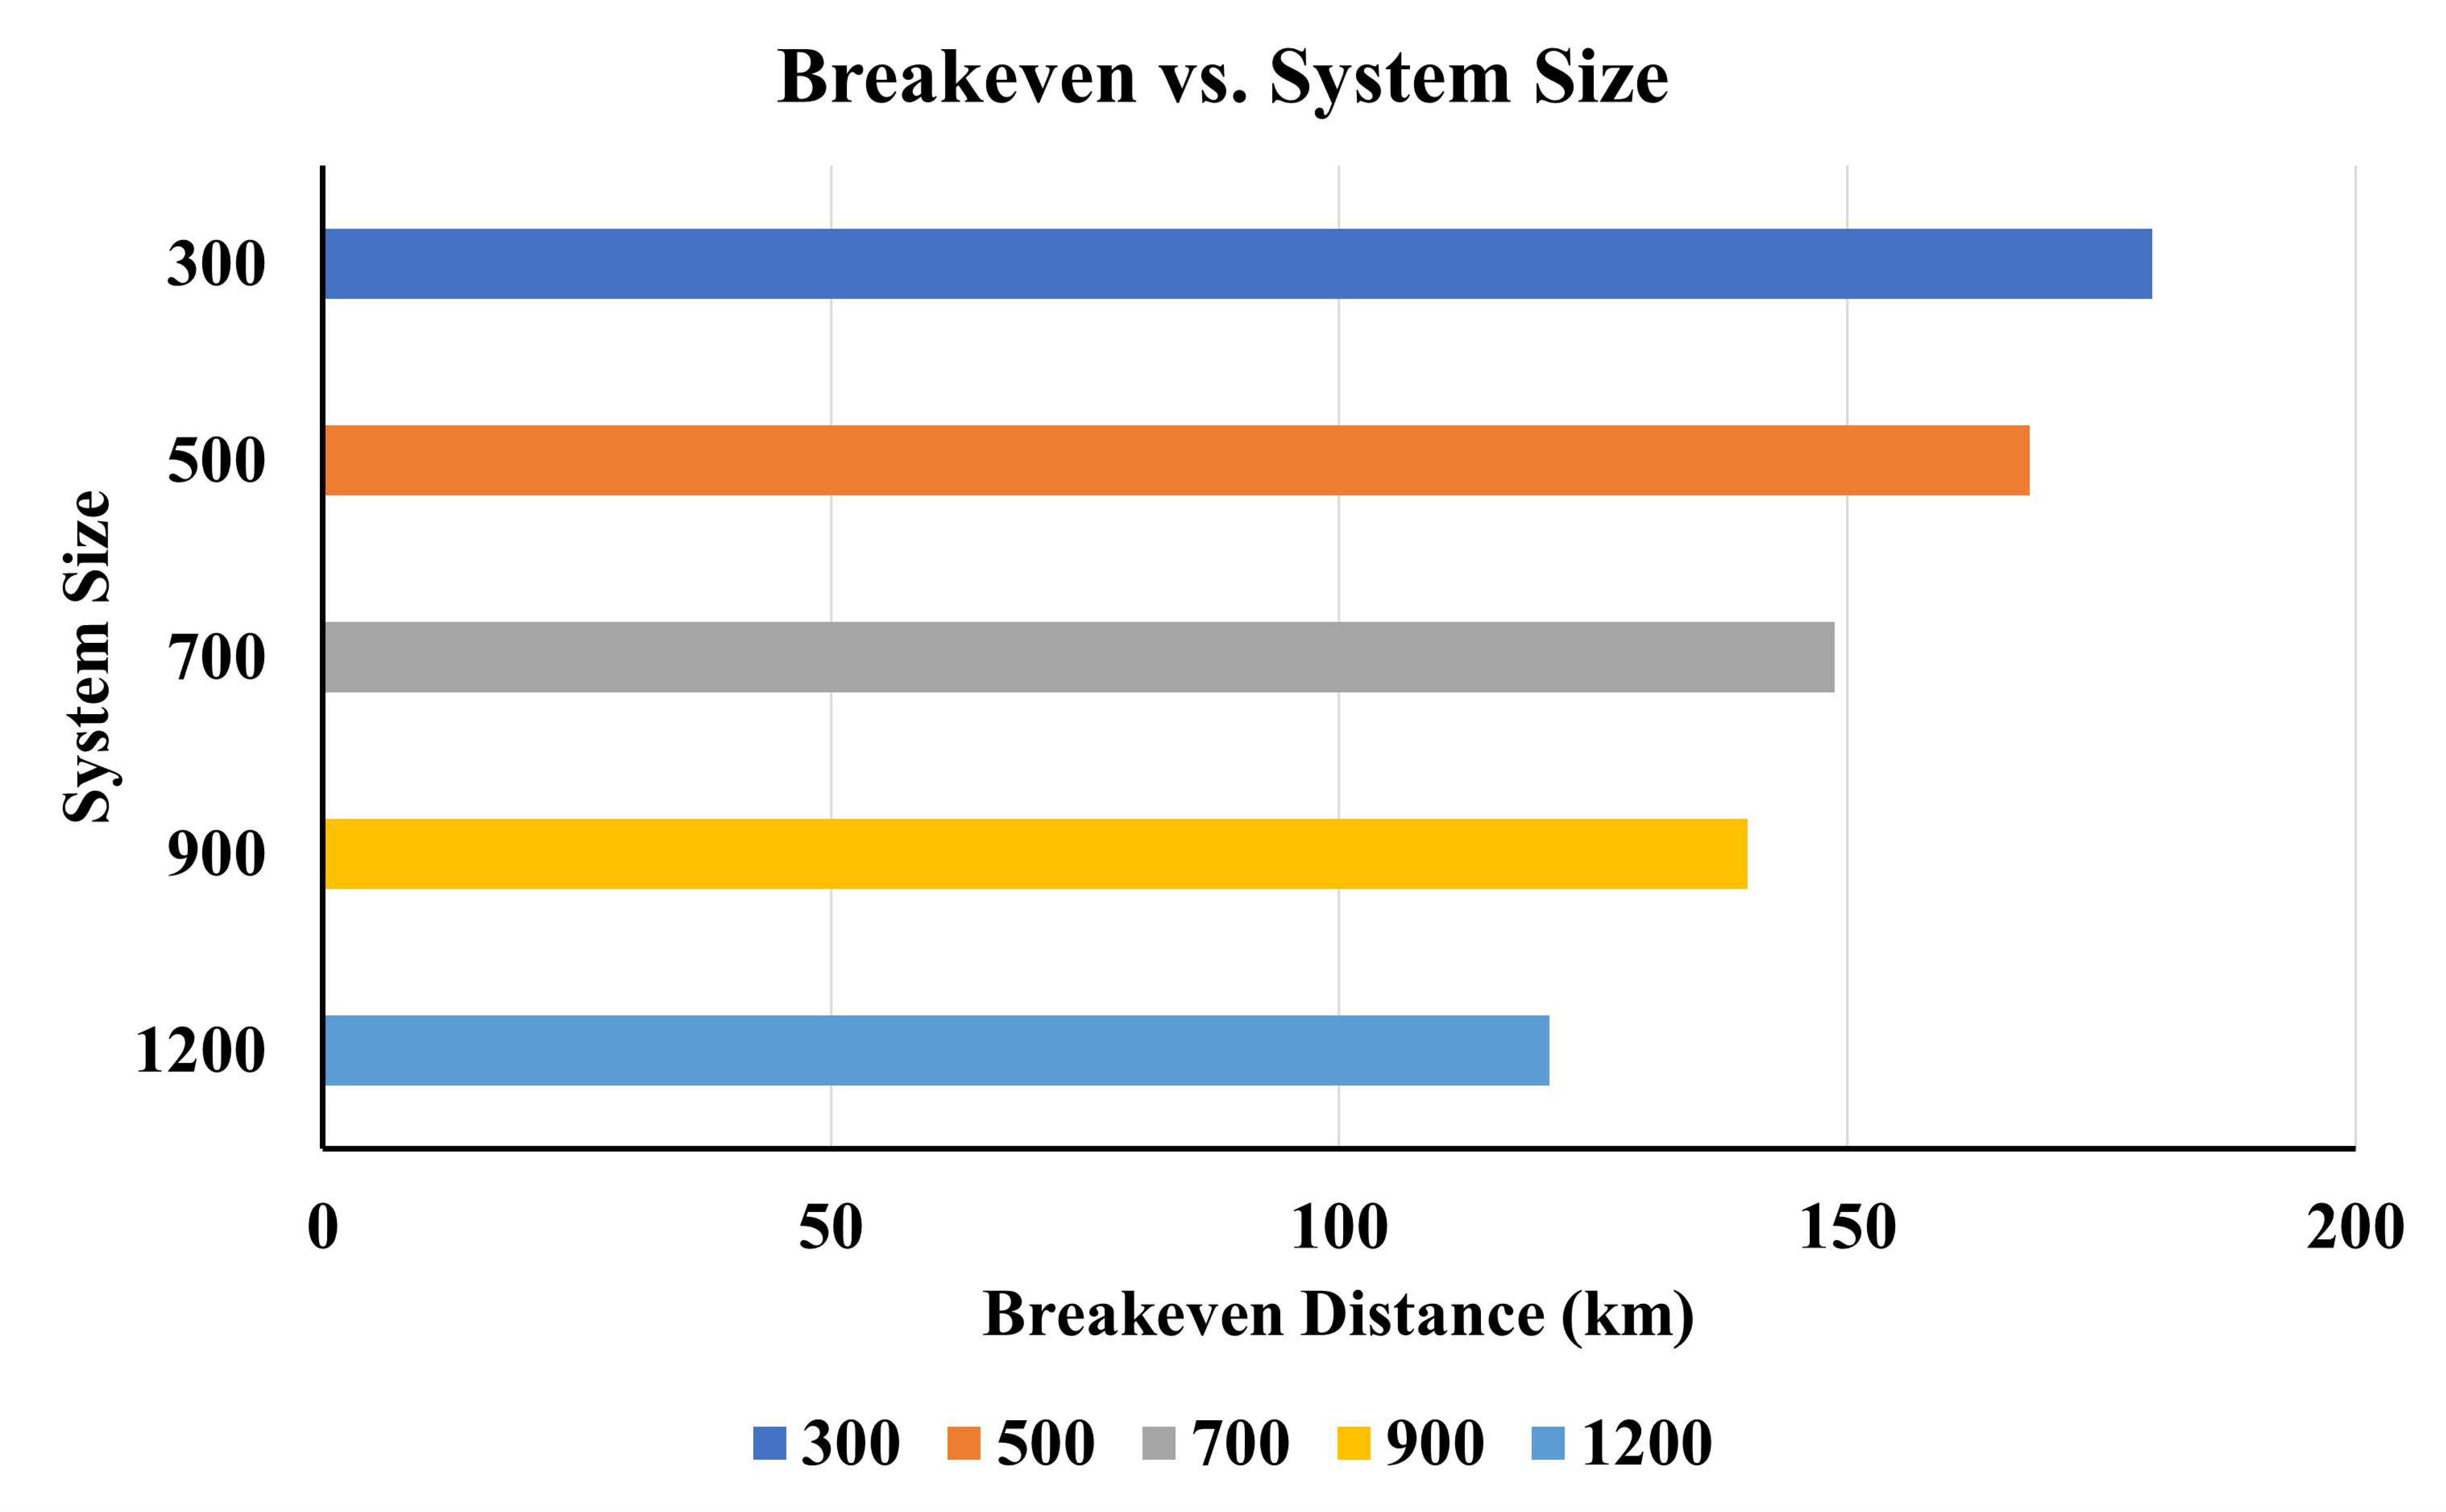
\includegraphics[scale=.37]{Figures/singh7.png}}
\caption{Breakeven Point with Considerations for Different Power Ratings.}
\label{fig final}
\end{figure}

The tradeoffs between HVDC and HVAC in offshore wind represent an essential consideration in developing OWF. However, offshore wind faces many headwinds beyond those related to the transmission system. Table \ref{economical challenge} describes some of the challenges opposing the development and integration of offshore wind systems and potential mitigation strategies. Long-term financing proves a perennial challenge for any significant offshore wind system due to the highly uncertain nature of the revenue stream and the highly variable cost of infrastructure projects \cite{garcia2017analysis,heeter2019international,welisch2020auctions,beiter2024enduring,jansen2022policy}.

Contracts for differences and renewable portfolio standards have gone a long way toward improving financing outcomes. Offshore wind penetration-- like all renewables penetration-- has the potential to exacerbate the missing money problem for base load and cause reliability challenges or price increases \cite{papalexopoulos2015modeling,mozdawar2022multiple,schiro2015convex,lamadrid2012ancillary,zou2021sustainable,kumar2019strategic,wang2018optimization,botterud2024bridging,gonzales2022dynamic}. Work toward improved capacity markets and convex hull pricing can help ensure funding for traditional generation. A sustainable supply chain remains essential for offshore wind as wind farm development is highly dependent on metals, and metals procurement is not without geopolitical risks and environmental costs \cite{li2022future,nguyen2022electric}.

The intermittency problem further poses challenges for grid planners, as does the issue of reliability and resilience to outages \cite{gao2024techno,wang2018optimization,tarufelli2022capacity,liu2022towards}. Finally, like any technology, offshore wind faces a learning curve as it transitions toward not just technological but commercial maturity. This will require initial support for workforce development and investments and could be challenged by the uncertainty of political environments related to funding and environmental policy \cite{ExecutiveOrder2007,schwabe2017wind,de2012assessing,stefek2022us,keyser2019wind,hu2018barriers,gowrisankaran2022policy}. Ultimately, all these challenges, though complex, are solvable and demonstrate the significant value of future collaboration between engineering and economic analysis.

 \subsection{\textbf{Economic Considerations for Reliability}}

Reliability creates another dimension of distinction between technologies. In the literature, there is a consensus that HVAC has the highest reliability, followed by VSC-HVDC and LCC-HVDC, with work being performed to improve reliability across all system types. DC/DC and DC/AC converters have significantly higher probabilities of failure than other components and also create outages of the entire generator rather than a specific cluster \cite{sun2021reliability}.

Based on estimates from the literature \cite{sun2021reliability,maciver2015reliability,li2021review,lakshmanan2021electrical,yang2022critical}, Table \ref{Failure} provides the likelihood of failure for different components within the OWF system, as well as the average Down Time (DT) for those components in an outage, and the yearly expected maintenance time of the components.


\begin{table}[htbp]
\caption{Failure Likelihood by Component}
\label{Failure}
 \renewcommand{\arrayrulewidth}{1.1pt}
 \arrayrulecolor{black}
 \renewcommand{\tabcolsep}{2pt}
 \renewcommand{\arraystretch}{1.1}
 \small
\centering
\begin{tabular}{|
p{1.9cm}<{\raggedright\arraybackslash}|
m{2.2cm}<{\centering}|
m{1.6cm}<{\centering}|
m{1.7cm}<{\centering}|}
\hline
\textbf{System} & \multicolumn{3}{l|}{\textbf{Reliability Measure}} \\
\hhline{|>{\arrayrulecolor{white}}-|>{\arrayrulecolor{black}}---}
\textbf{Component} & {\bfseries P(Failure)} & {\bfseries DT (hrs)} & {\bfseries DT per Year} \\
\hline
\textbf{Generator} & 0.01-0.1 & NA & NA \\
\hline
\textbf{Transformer} & 0.0108-0.03 & 1440-4320 & 15.552-1296 \\
\hline
\textbf{AC Breaker} & 0.0015-0.025 & NA & NA \\
\hline
\textbf{DC Breaker} & 0.0033-0.025 & 240 & 0.792-6 \\
\hline
\textbf{AC/DC Converter} & 0.1 & NA & NA \\
\hline
\textbf{DC/DC Converter} & 0.014-0.613 & NA & NA \\
\hline
\textbf{Full Power Converter} & 0.05-0.2 & 720 & 36-144 \\
\hline
\textbf{DC Cables} & 0.0706 & 1440 & 101.67 \\
\hline
\textbf{AC Cables} & 0.0001-0.008/km & 2160 & 0.216-17.28 \\
\hline
\multicolumn{4}{l}{}
\end{tabular}
\end{table}




Typical models of reliability of OWF utilize assumed independent Poisson likelihood functions for individual components to perform Monte-Carlo simulations of the likelihood of total failure rather than an individual cluster. Most of these models do not consider potential external variables and potential dependence in the distributions of failures of multiple components.

The prior literature has not taken into account market considerations related to reliability. While the likelihood of failure of different components and the time to repair these components is determined, a valuation has not yet been put on the cost of downtime either for the generator or for the system as a whole. Further research could focus on quantifying average revenue losses from reliability failures and the associated costs to the grid system over the lifetime of the OWF. Developing a comprehensive revenue model would enable a more accurate determination of the breakeven point between HVDC and HVAC systems, considering the varying levels of reliability that research indicates directly influence costs.


\section{\textbf{OWF Connection Architectures}}

\begin{figure}[htbp]
\centerline{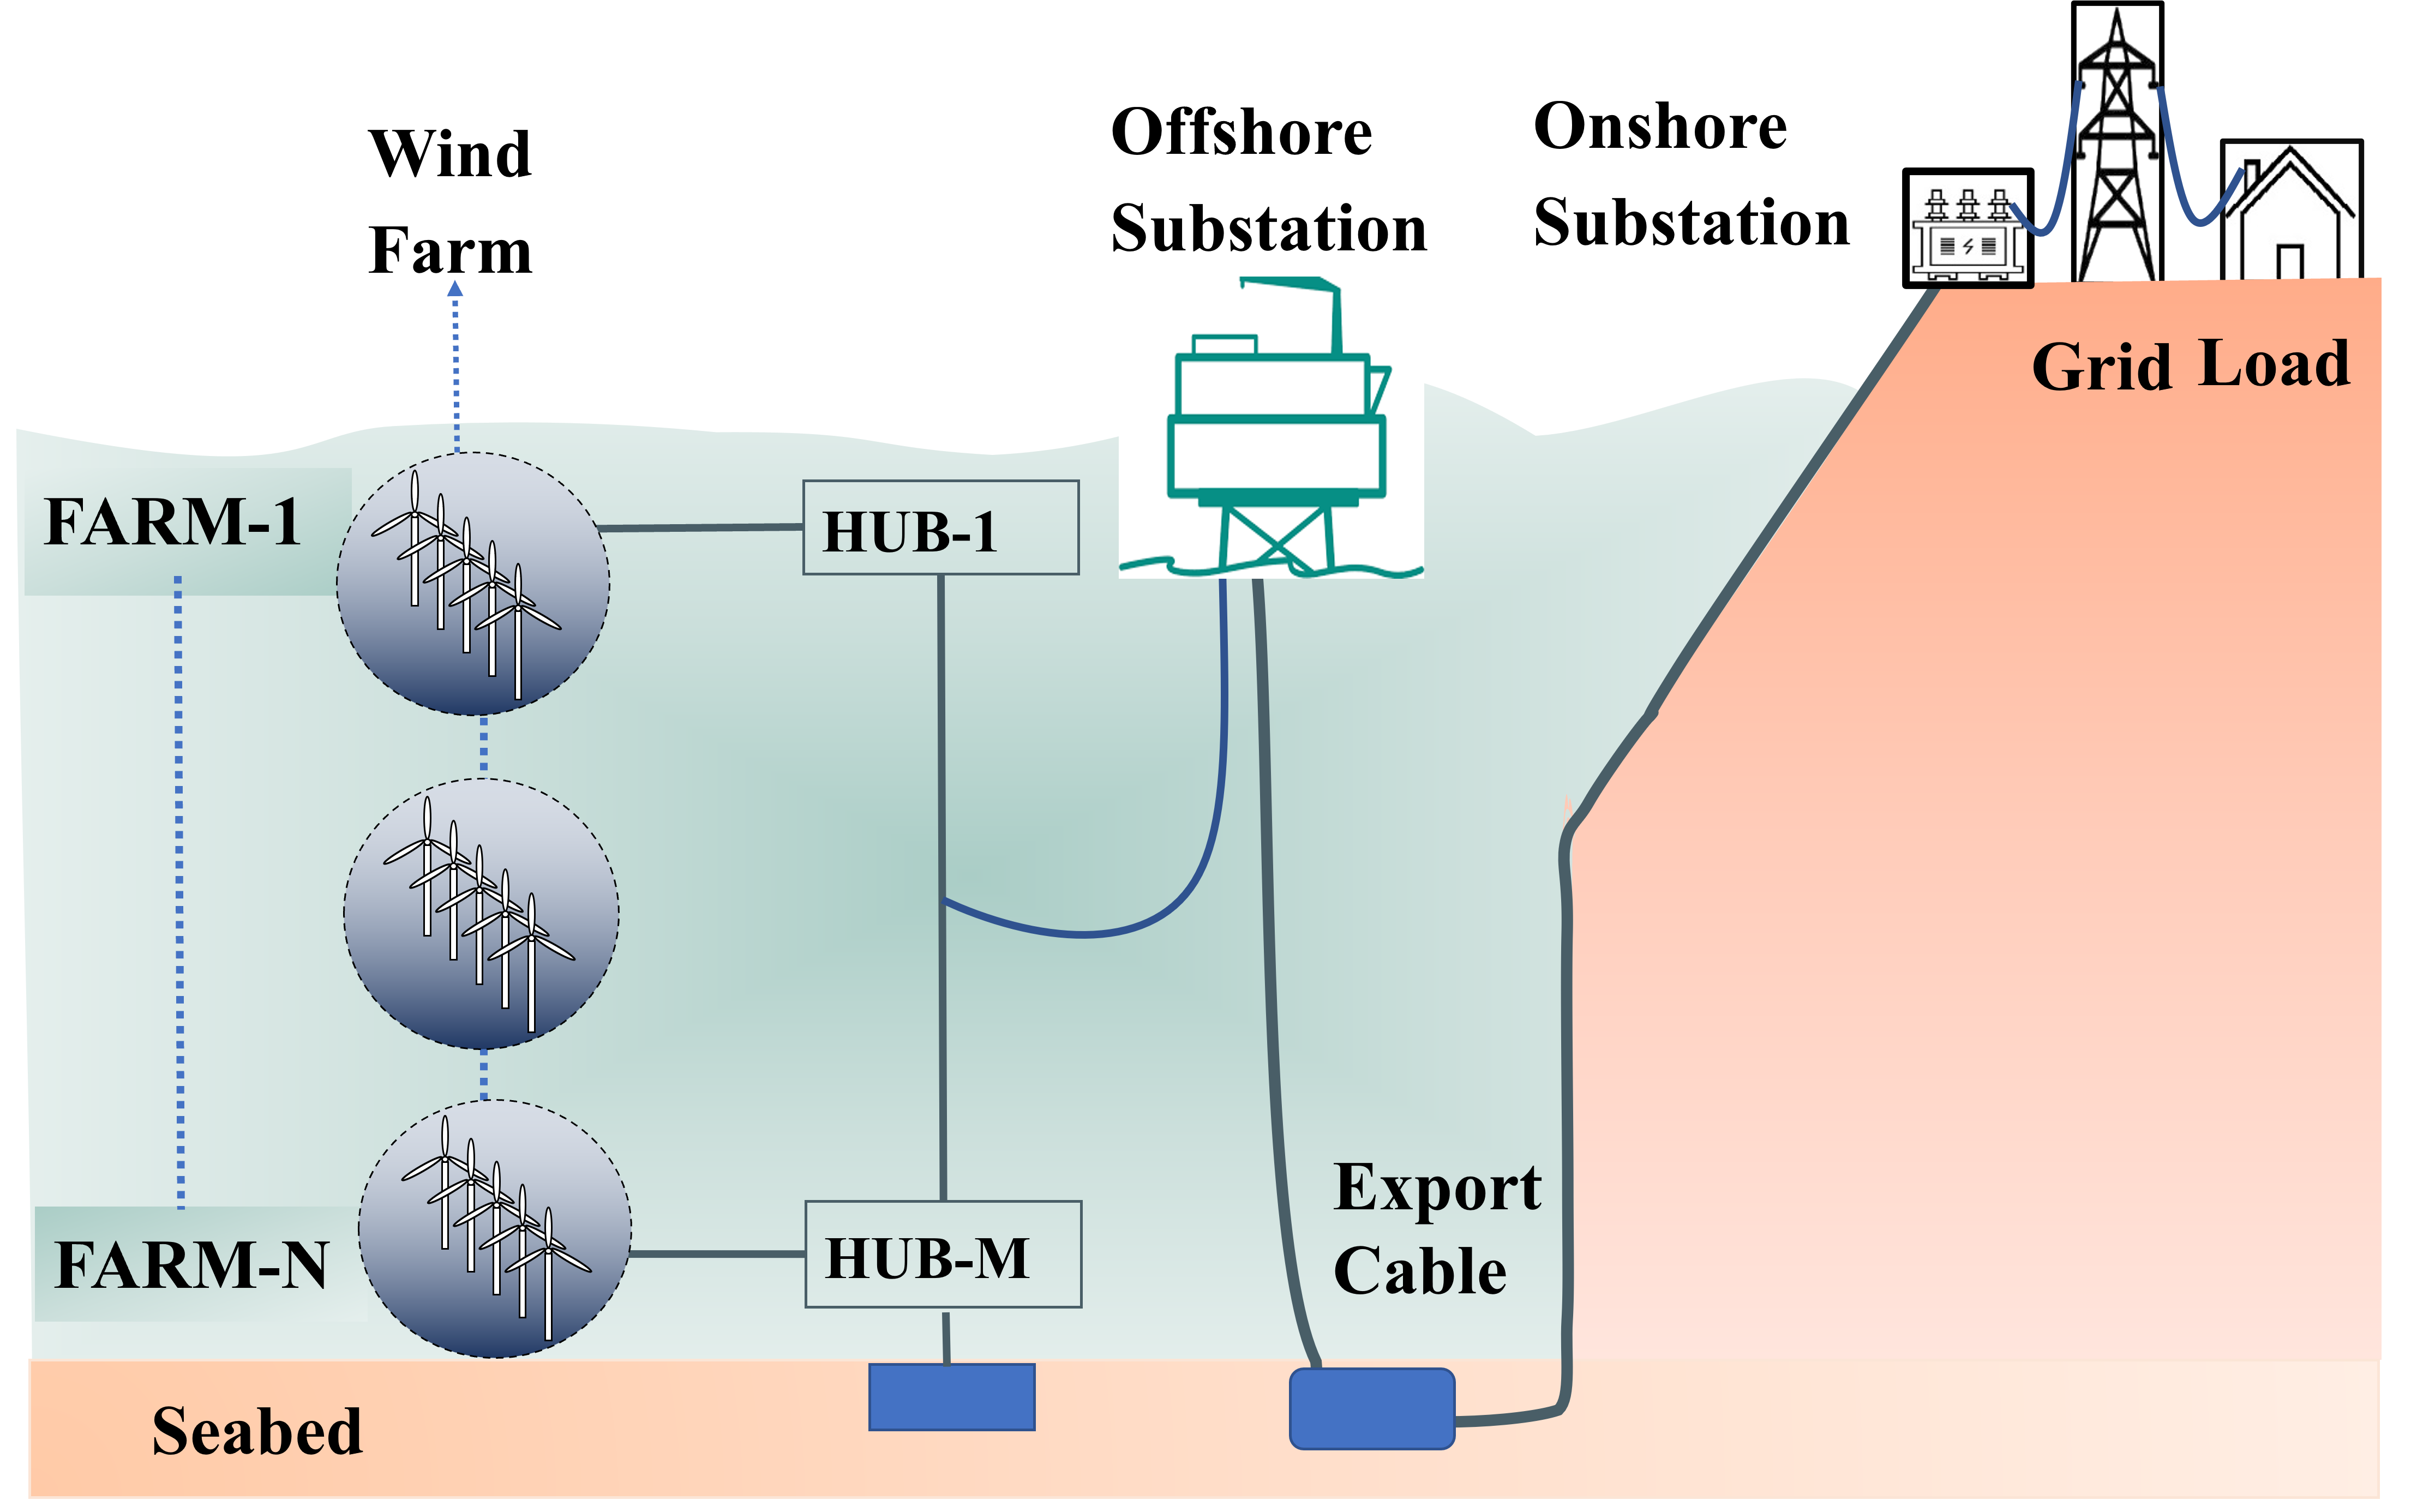
\includegraphics[width=3.3in]{Figures/singh8.png }}
\caption{Connection Layout of Grid-Tied Offshore Wind Farm.}
\label{Schematic.}
\end{figure}

\begin{figure}[htbp]
\centerline{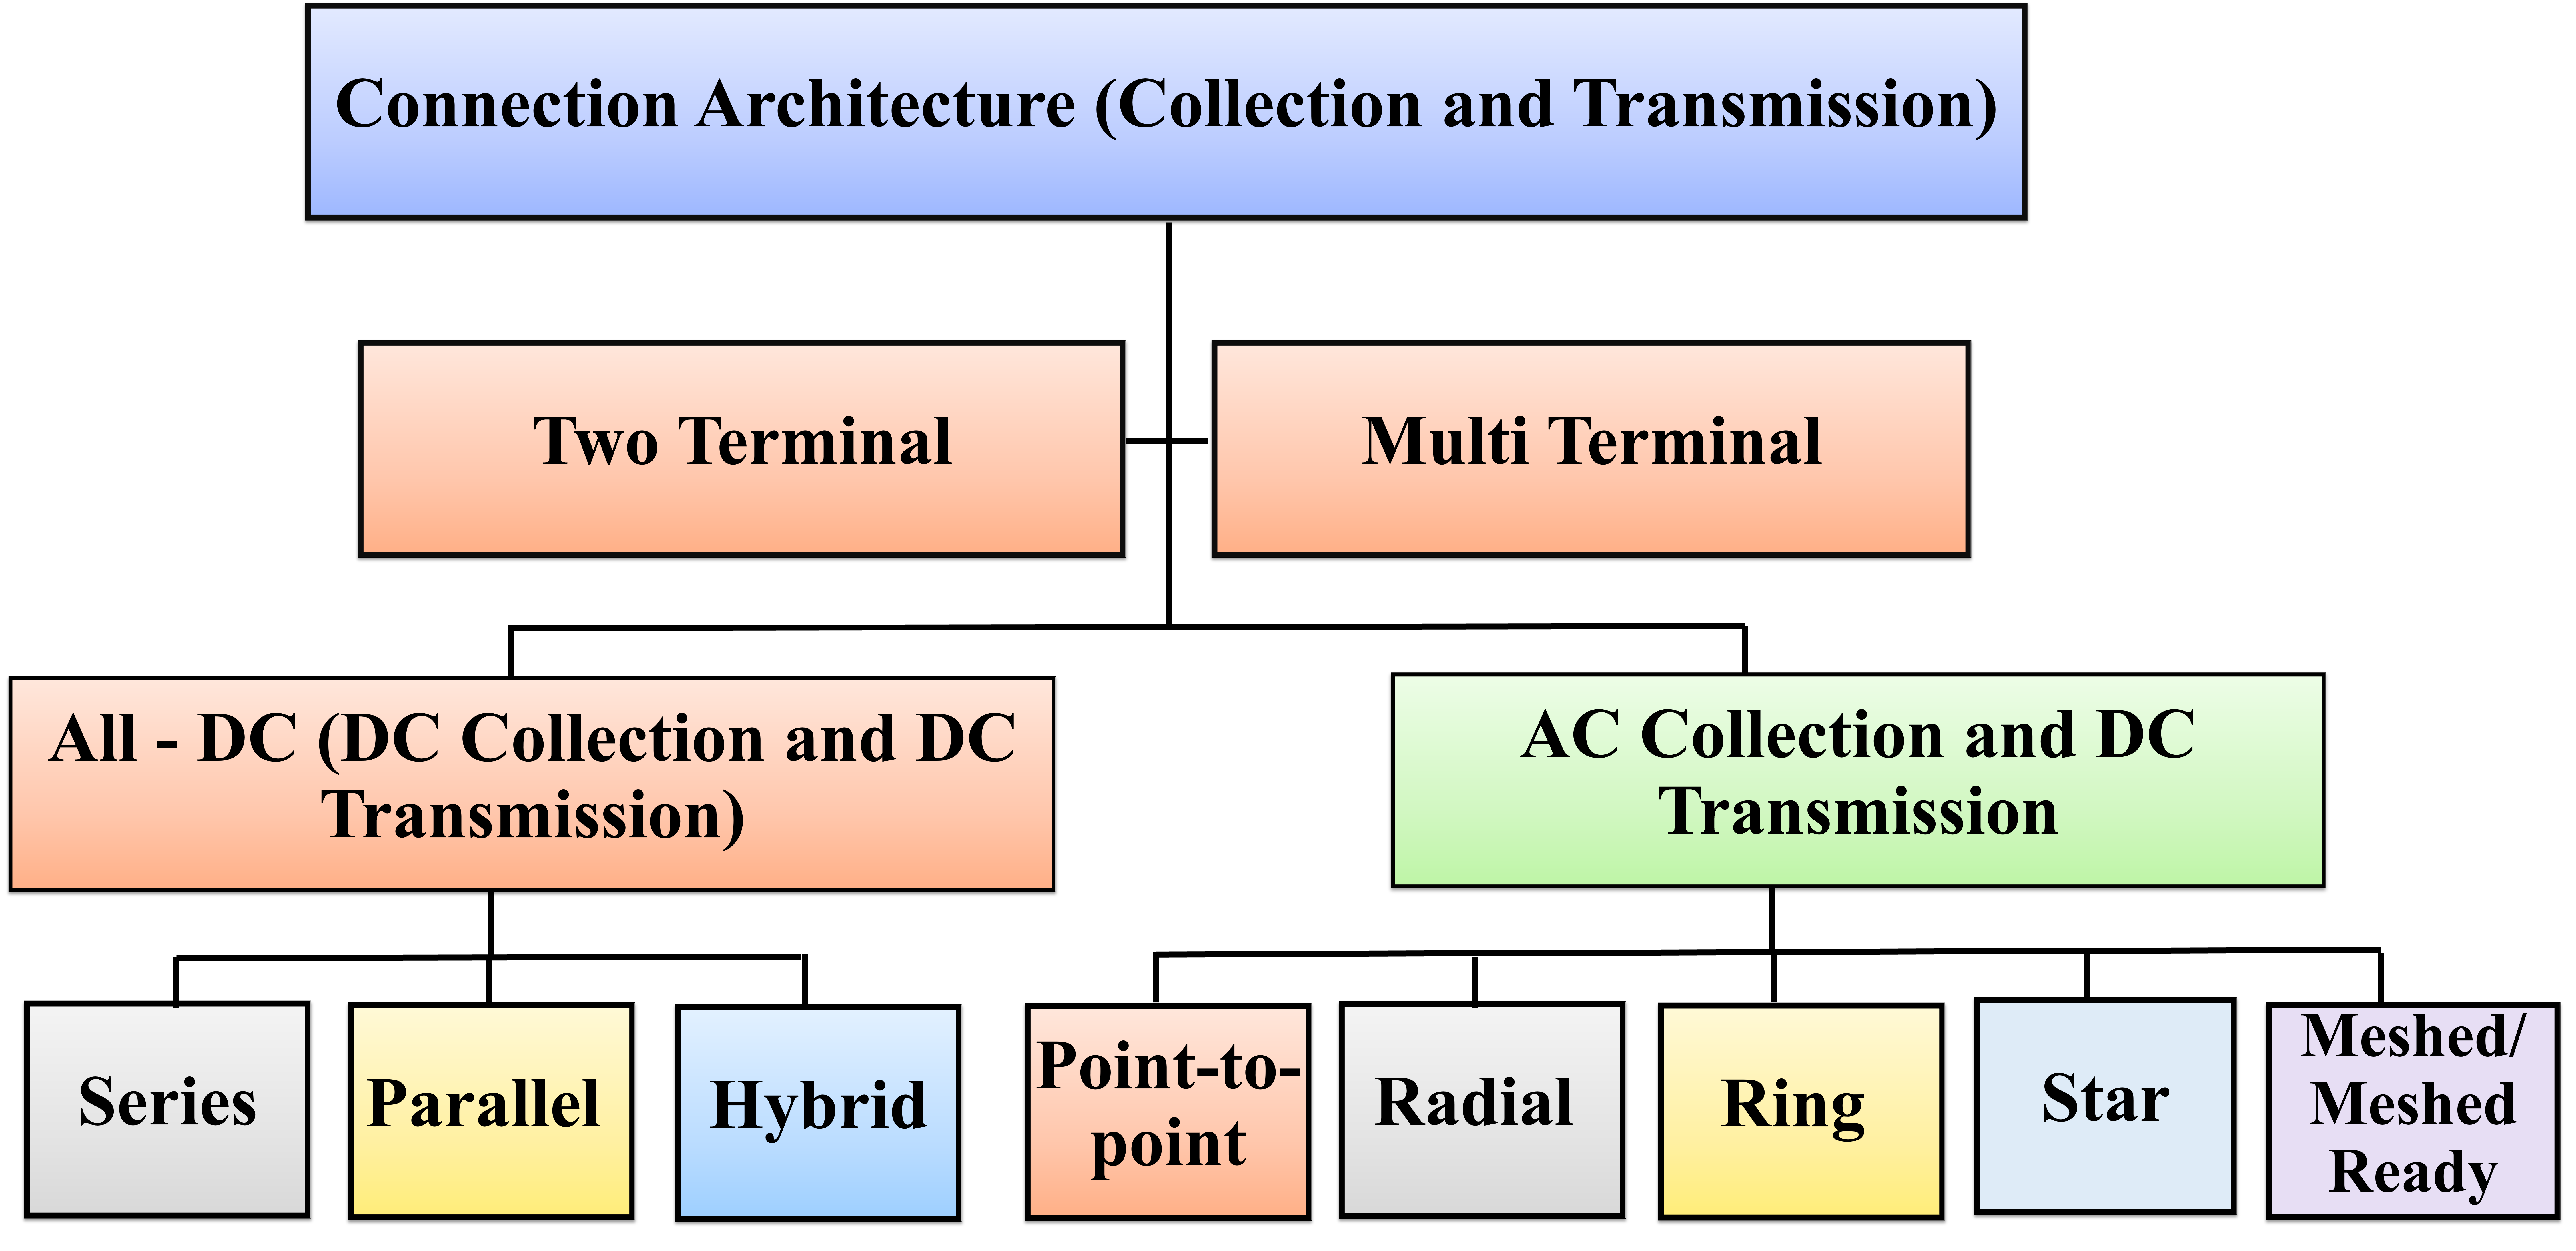
\includegraphics[width=3.3in]{Figures/singh9.png }}
\caption{Classification of Connection Topology.}
\label{Schematic of grid}
\end{figure}

\begin{figure}[htbp]
\centerline{\includegraphics[width=3.3in]{Figures/singh10.png }}
\caption{Schematic of Grid-Tied HVDC Offshore Wind Farm.}
\label{Schematic of grid1}
\end{figure}





The efficient gathering and transmission of power from OWFs constitute a critical aspect influencing their overall performance and economic viability. Fig. \ref{Schematic.}  illustrates the comprehensive connection layout of the OWFs, representing all the electrical components that connect the wind turbine output to the onshore power grid. This includes generating units, power electronic converters, transformers, inter-turbine cables, transmission cables, and switch gears. This electrical infrastructure operates through two primary sections that define the power transfer networks \cite{madariaga2012current}. The first section, known as the collection system, interconnects the wind turbines within the OWFs. Meanwhile, the second section, the transmission system, plays a pivotal role by establishing the vital link between the offshore and the onshore grid, often operating at elevated voltage levels.

Offshore wind turbines generate electricity individually, and the generated power must be collected and aggregated prior to transmission. Collection systems, often consisting of subsea cables, gather the electricity from multiple turbines within an array and transmit it towards a central point \cite{lundberg2006evaluation}. \cite{lakshmanan2021electrical} addresses the related research on different OWF collection systems and explores their operational characteristics and challenges. 

The architecture of the collection grid can be either AC or DC based on the type of energy source and the location of the offshore farm \cite{madariaga2013technological, rahman2021comparison}. \cite{lakshmanan2015assessment} provides a technical and economic comparative analysis between DC and AC collection systems for OWFs, highlighting that while DC systems offer size and weight reductions, they face higher costs and losses compared to AC systems due to the need for DC protection devices and converters. 

In this review paper, our primary focus revolves around various collection architectures designed for HVDC transmission in OWFs. Fig. \ref{Schematic of grid} presents potential connection architectures for OWFs, such as AC collection combined with DC transmission and all DC-based systems. Meanwhile, Fig. \ref{Schematic of grid1} provides a general schematic of a grid-connected HVDC OWF, highlighting the voltage ratings at key points throughout the system.%illustrates a general schematic of the HVDC grid architecture specifically designed for OWFs.
\subsection{\textbf{AC Collection Architecture}}

\begin{figure}[htbp]
\label{AC Collection Fig}
\centerline{\includegraphics[width=3.5in]{Figures/singh11.png }}
\caption{AC Collection Architecture.}
\label{AC collection}
\end{figure}

% Please add the following required packages to your document preamble:
% \usepackage{multirow}
\begin{table*}[htbp]
\caption{Comparison of AC Collection Grid Architectures}
\renewcommand{\arrayrulewidth}{1.1pt} % Increase border thickness
\arrayrulecolor{black}
\renewcommand{\arraystretch}{1.3} % Increase row height for better readability
\centering
\small
\label{compare AC}
\begin{tabular}{|
p{2.1cm}<{\raggedright\arraybackslash} |
p{2.8cm}<{\raggedright\arraybackslash}|
p{3.3cm}<{\raggedright\arraybackslash} |
p{3.6cm}<{\raggedright\arraybackslash}|
p{3.2cm}<{\raggedright\arraybackslash}|}
\hline
\textbf{Aspect} &
  \textbf{Point-to-Point} &
  \textbf{Radial} &
  \textbf{Ring} &
  \textbf{Star} \\ \hline
\textbf{Topology} &
  \begin{tabular}[]{@{}l@{}}$-$ Direct connection to \\ \hspace{8pt}a central substation\end{tabular} &
   \begin{tabular}[]{@{}l@{}}$-$ Single path linear \\ \hspace{8pt}structure \end{tabular} &
  \begin{tabular}[]{@{}l@{}}$-$ Circular loop with \\ \hspace{8pt} multiple interconnections\end{tabular} &
  \begin{tabular}[]{@{}l@{}}$-$ Multiple units connect- \\ \hspace{8pt}ed to a central hub\end{tabular} \\ \hline
 &
  $-$ Limited &
  $-$ Limited &
  $-$ Moderate &
  $-$ High \\ \hhline{|>{\arrayrulecolor{white}}-|>{\arrayrulecolor{black}}----}
\multirow{-2}{*}{\begin{tabular}[]{@{}l@{}}\textbf{Redundancy} \\\&  \textbf{Reliability}\end{tabular}} &
  \begin{tabular}[]{@{}l@{}}$-$ Single fault disrupts \\\hspace{8pt}the  connected unit\end{tabular} &
  \begin{tabular}[]{@{}l@{}}$-$ Fault affects down- \\\hspace{8pt}stream units \end{tabular} &
  \begin{tabular}[]{@{}l@{}}$-$ Faults in one segment \\ \hspace{8pt} may not impact the loop\end{tabular} &
  \begin{tabular}[]{@{}l@{}}$-$ Centralized hub  \\ \hspace{8pt} reduces fault impacts\end{tabular} \\ \hline
\textbf{Control} &
  \begin{tabular}[]{@{}l@{}}$-$ Simplified voltage \\ \hspace{8pt}control at the sub- \\ \hspace{8pt}station\end{tabular} &
  \begin{tabular}[]{@{}l@{}}$-$ Easy control with \\ \hspace{8pt}possible voltage drops \\ \hspace{8pt} along the path\end{tabular} &
  \begin{tabular}[]{@{}l@{}}$-$ Partial voltage control \\ \hspace{8pt} through loop paths\end{tabular} &
  \begin{tabular}[]{@{}l@{}}$-$ Centralized, robust \\ \hspace{8pt}voltage control\end{tabular} \\ \hline
\textbf{Scalability} &
  \begin{tabular}[]{@{}l@{}}$-$ Low; significant \\ \hspace{8pt}adjustments needed\end{tabular} &
  \begin{tabular}[]{@{}l@{}}$-$ Limited; requires new \\ \hspace{8pt}connections\end{tabular} &
  $-$ Moderate via loop paths &
  \begin{tabular}[]{@{}l@{}}$-$ Highly scalable; units \\\hspace{8pt} easily added to the hub\end{tabular} \\ \hline
\begin{tabular}[]{@{}l@{}}\textbf{Complexity}\\\&  \textbf{Cost}\end{tabular} &
  \begin{tabular}[]{@{}l@{}}$-$ Simple design; \\ \hspace{8pt}lower initial cost\end{tabular} &
  \begin{tabular}[]{@{}l@{}}$-$ Simple design;\\ \hspace{8pt} added cost for \\ \hspace{8pt} voltage \& reliability \end{tabular} &
  \begin{tabular}[]{@{}l@{}}$-$ Moderate due to loop setup\end{tabular} &
  \begin{tabular}[]{@{}l@{}}$-$ High, but better \\\hspace{8pt} redundancy\end{tabular} \\ \hline
\textbf{Suitability} &
  \begin{tabular}[]{@{}l@{}}$-$ Best for small\\ \hspace{8pt} systems with\\ \hspace{8pt} limited growth\end{tabular} &
  \begin{tabular}[]{@{}l@{}} $-$For small to medium \\ \hspace{8pt}systems \end{tabular} &
  \begin{tabular}[c]{@{}l@{}}$-$ Ideal for medium install-\\ \hspace{8pt}ations with room for \\ \hspace{8pt}expansion\end{tabular} &
  \begin{tabular}[]{@{}l@{}}$-$ Best for large, complex,  \\ \hspace{8pt} or expanding systems\end{tabular} \\ \hline
\end{tabular}
\end{table*}





In AC collection grids, the electrical power generated by OWF devices is stepped up to a higher voltage level for efficient transmission to onshore substations \cite{timmers2023all}. AC grids offer several benefits, including mature technology, high efficiency, and seamless integration with existing electrical networks \cite{fjellstedt2022review, le2020unidirectional}. Depending on the size of the wind farm and its distance from the shore, different topologies are employed to optimize power collection and ensure system reliability. Each topology presents specific advantages and limitations, tailored to suit particular wind farm layouts and their proximity to the coast \cite{lakshmanan2021electrical}. Fig. \ref{AC collection} provides an overview of various AC collection-based topologies utilized in HVDC transmission systems.



\begin{figure}[htbp]
\centerline{\includegraphics[width=3.3in]{Figures/singh12.png }}
\caption{DC Series Collection Architecture.}
\label{DC Collection}
\end{figure}
\subsubsection{\textbf{Point-to-Point}} The point-to-point topology consists of direct connections between individual offshore energy generation units and the shore, with each unit independently linked through its transmission cable \cite{glasdam2013hvdc}. Although this design offers simplicity in both implementation and operation, it requires many individual cables, leading to higher installation and maintenance costs. As a result, it is not well suited for large-scale wind farms. Furthermore, the point-to-point configuration lacks the flexibility to facilitate power exchange between multiple areas or regions, limiting its adaptability to interconnected systems \cite{zhang2016review}.

\subsubsection{\textbf{Radial}} The radial topology uses a "daisy-chain” configuration, where the cable capacity increases progressively after each connected unit. This design minimizes costs by requiring fewer cables and simpler infrastructure. However, it is vulnerable to single-point failures, compromising system reliability. To connect multiple units, hubs, junctions, or low-/medium-voltage transformers are typically used \cite{maciver2015reliability}.

\subsubsection{\textbf{Ring}} The ring topology interconnects units through looping cables, creating a circular arrangement \cite{korompili2016review}. Although the ring design adds complexity and higher costs due to the need for additional switches and cabling, it significantly enhances reliability. In the event of a fault, the two-way power flow within the loop ensures continued operation, making it more robust than a radial system \cite{rahman2021comparison}.

\subsubsection{\textbf{Star}} In the star topology, units are grouped and connected to a central hub using cables of similar ratings, with the collected power transmitted to shore through higher-rated cables \cite{raza2020multi}. This design simplifies the connection process and allows individual control of each turbine. However, a hub failure can impact all connected turbines, reducing the reliability of the system. While the star topology can be cost-effective for smaller-scale systems, both cost and complexity increase for larger systems due to the central hub's location and associated infrastructure. A similar cluster-based architecture is described in \cite{li2021review}.

Table \ref{compare AC} offers a detailed comparison of different AC collection grid architectures. It evaluates their performance across several key parameters, including redundancy, reliability, voltage levels, transmission distance, complexity, cost, scalability, and adaptability for seamless integration with offshore wind systems. 

\subsection{\textbf{Limitations of AC Collection Grids}}

\begin{table*}[htbp]
\caption{Integration Challenges of OWFs}
 \renewcommand{\arrayrulewidth}{1.1pt}
 \renewcommand{\arraystretch}{1.2} % Increase row height
 \arrayrulecolor{black}
 \small % Increase font size
\centering
\label{technical_challenge}
\begin{tabular}{|
p{2.2cm}<{\raggedright\arraybackslash}|
p{4.5cm} <{\raggedright\arraybackslash}|
p{7.5cm} <{\raggedright\arraybackslash}|
p{1.6cm} <{\raggedright\arraybackslash}|}
\hline
\multicolumn{2}{|l|}{\textbf{Main Challenge}} & \textbf{Mitigation Strategy} & \textbf{References} \\ \hline
 & Harmonic Distortion & \begin{tabular}[]{@{}l@{}}$-$Use of active/passive filters \\ $-$Advanced Control Algorithms\end{tabular} & \cite{nami2018active,zhang2021study,karlsson2023managing} \\ \hhline{|>{\arrayrulecolor{white}}-|>{\arrayrulecolor{black}}---}
 & Voltage Unbalance & \begin{tabular}[]{@{}l@{}}$-$Dynamic voltage balancing techniques \end{tabular} & \cite{schonleber2017handling} \\ \hhline{|>{\arrayrulecolor{white}}-|>{\arrayrulecolor{black}}---}
\multirow{-3}{*}{\textbf{Power Quality}} & Voltage Sag, Swell, Flickers & \begin{tabular}[c]{@{}l@{}}$-$Use of FACTS devices \\ $-$ Dynamic VAR compensators\\ $-$ Power conditioning systems.\end{tabular} & \cite{ferdinand2018power,almohaimeed2020power} \\ \hline
\multirow{3}{*}{\textbf{Stability}} & Voltage Stability & \begin{tabular}[]{@{}l@{}}$-$Reactive power compensation \\ $-$Advanced Control Techniques \\ $-$Turbine converters with reactive power control\end{tabular} & \cite{lee2020dc} \\ \hhline{|>{\arrayrulecolor{white}}-|>{\arrayrulecolor{black}}---}
 & Frequency Stability & \begin{tabular}[]{@{}l@{}}$-$De-loading by Variable Speed Wind Turbine \\ $-$Capacitor energy storage in VSC-HVDC \\ $-$Coordinated Frequency Control of OWF \& VSC-HVDC\end{tabular} & \cite{jallad2017frequency} \\ \hhline{|>{\arrayrulecolor{white}}-|>{\arrayrulecolor{black}}---}
 & \begin{tabular}[]{@{}l@{}}Fault Ride-Through Capability \\ (LVRT/HVRT)\end{tabular} & \begin{tabular}[]{@{}l@{}}$-$Implement LVRT and HVRT schemes in wind \\  \hspace{8pt}turbines \& HVDC converters\end{tabular} & \cite{jia2023harmonic} \\ \hline
\multirow{1}{*}{\shortstack{\textbf{Fault Diagnosis} \\ \textbf{\& Protection}}} & Offshore Converter Protection & \begin{tabular}[]{@{}l@{}} $-$ Use of advanced protection systems \& \\ \hspace{8pt} fault detection technologies \end{tabular} & \cite{chao2024high,li2018new,mitra2018hvdc,ashrafi2023intelligent} \\ \hhline{|>{\arrayrulecolor{white}}-|>{\arrayrulecolor{black}}---}
 & Short-Circuit Current Limitation & \begin{tabular}[]{@{}l@{}}$-$Use of superconducting fault current limiters\\ $-$Adaptive relays; precise fault detection and response\end{tabular} & \cite{guerreiro2023concerning,song2022novel,qin2020review} \\ \hline
\textbf{Inertia} & System Inertia Reduction & \begin{tabular}[]{@{}l@{}}$-$Use of synthetic inertia from wind turbine control \\ $-$ESS-based inertia emulation \\ $-$Virtual synchronous machines to mimic inertia\end{tabular} & \cite{zeng2021approach,tu2021synthetic,zhu2024supercapacitor} \\ \hline
& Frequency Regulation & \begin{tabular}[]{@{}l@{}} $-$ Battery Energy Storage Systems (BESS) \\ $-$ Synthetic inertia for fast frequency response \\ $-$ Advanced control algorithms \end{tabular} & \cite{bidadfar2020feasibility,lin2020overview,kabsha2019new} \\ \hhline{|>{\arrayrulecolor{white}}-|>{\arrayrulecolor{black}}---}
\multirow{1}{*}{\shortstack{\textbf{Ancillary Service} \\\hspace{-9pt}\textbf{Provision}}} &Voltage \& Reactive Power Control & \begin{tabular}[]{@{}l@{}}$-$Use of FACTS devices (STATCOM, SVC) \\ $-$Wind turbine converters with reactive power support\end{tabular} & \cite{wu2023overview,tanaka2018asymmetrical,meng2024communication,gupta2022improved} \\ \hhline{|>{\arrayrulecolor{white}}-|>{\arrayrulecolor{black}}---}
 & Provision of Reserve Power & \begin{tabular}[]{@{}l@{}}$-$Novel large-scale ESS \\ $-$Coordinated operation with other RES\end{tabular} & \cite{jiang2023thermodynamic,hellesnes2017use,rabanal2024energy,kluger2023power} \\ \hhline{|>{\arrayrulecolor{white}}-|>{\arrayrulecolor{black}}---}
 & Black Start Capability & \begin{tabular}[]{@{}l@{}}$-$Implement black start capability in ESS \\ $-$Specific turbines designed for black start operations \\ $-$Coordinated black-start strategy\end{tabular} & \cite{pagnani2023integrating,liu2023mmc,pagnani2020offshore,tang2024coordinated} \\ \hline
\multirow{1}{*}{\shortstack{\textbf{Converter Sizing} \\ \textbf{\& Efficiency}}} & Converter Weight and Volume & \begin{tabular}[]{@{}l@{}}$-$Use of modular multilevel converters (MMC) \\ $-$Advanced materials to reduce size and weight \\ $-$Novel collection systems\end{tabular} & \cite{diaz2020overview,ghassemi2020high,zhou2023review,follo2021challenges} \\ \hhline{|>{\arrayrulecolor{white}}-|>{\arrayrulecolor{black}}---}
 & Converter Losses & \begin{tabular}[]{@{}l@{}}$-$Use of high-efficiency semiconductor technologies \\ \hspace{8pt} (e.g., SiC or GaN) \\ $-$Advanced converter topologies for lower losses\end{tabular} & \cite{tian2024novel,garces2010impact} \\ \hline
\textbf{Grid Code Compliance} & Compliance with Grid Codes & \begin{tabular}[]{@{}l@{}}$-$Adaptive control schemes to meet diverse grid codes \\ $-$Ensuring LVRT/HVRT capabilities\end{tabular} & \cite{mishra2025grid,kabsha2022adaptive} \\ \hline
\end{tabular} 
\end{table*}


AC grids, known for their mature technology, high efficiency, and seamless integration, have long served as the backbone of onshore and offshore power transmission. However, integrating large-scale OWFs into AC grids presents unique challenges due to the fluctuating power output, extended transmission distances, and complex synchronization requirements with onshore grids. These factors amplify critical issues such as voltage instability, harmonic distortions, and reactive power management, which are crucial to maintaining reliable grid operations \cite{lundberg2006evaluation, ali2021offshore, campos2018offshore}. Table \ref{technical_challenge} lists the challenges and their mitigation strategies.


In offshore environments, AC collection grids encounter additional technical and operational challenges stemming from the reactive nature of AC power. Long transmission distances introduce capacitive effects in submarine cables, leading to a reactive power imbalance. Shunt reactors and Static Synchronous Compensators (STATCOMs) are deployed to manage these effects. While effective, these approaches increase system complexity and operational costs \cite{kushwaha2023review}. 

Voltage regulation becomes more difficult as the transmission distance increases, requiring additional equipment to maintain stability \cite{rehman2023critical}. Furthermore, power converters and switching operations in AC systems generate harmonics, which demands sophisticated filtering solutions to ensure that power quality is not compromised \cite{ruiz2021wind}. These technical hurdles make the design, operation, and maintenance of AC systems for OWFs more complex and expensive.

Moreover, a key limitation of AC collection systems is the large size and footprint required for offshore substations, further complicating their deployment and scalability \cite{lakshmanan2021electrical}. AC substations need bulky components such as transformers, reactors, switchgear, and harmonic filters to manage voltage levels and reactive power \cite{pillay2021comparative}. This increases the weight of offshore platforms, making construction and installation costly and logistically challenging. The platforms must not only support heavy equipment, but also withstand harsh marine conditions, further raising the cost and limits the scalability of the infrastructure. Furthermore, as OWFs increase in size and move farther from shore, the economic and logistical challenges of AC systems become even more pronounced \cite{yang2022critical}.

\subsection{\textbf{Transition from AC to DC Collection Systems}}

To address the limitations of AC systems, research has increasingly emphasized the development of DC collection grids and All-DC systems for OWFs \cite{timmers2023all}. DC systems offer several advantages over AC infrastructure, particularly for long-distance, high-capacity power transmission \cite{musasa2017review}. One of the most notable benefits is the elimination of reactive power compensation, as DC transmission does not involve reactive power \cite{abeynayake2019review}. This allows for the removal of large transformers, reactors, and compensation devices, resulting in smaller, lighter substations with a reduced physical and environmental footprint \cite{follo2021challenges}.

DC systems also simplify grid integration by reducing the number of conversion stages and minimizing harmonic distortion \cite{karlsson2023managing}. In an All-DC setup, wind turbines generate DC power directly, which can be transmitted to the shore without need for AC / DC conversion at the wind farm level, improving efficiency and reliability \cite{song2022modular}. With fewer components required for voltage and power quality management, DC grids reduce operational complexity and maintenance needs, making them more suitable for large-scale offshore installations.


In summary, while AC grids have been the cornerstone of power infrastructure, their limitations in offshore applications have accelerated the shift toward DC collection grids and HVDC systems. DC systems provide a promising solution to address the challenges of power quality, reactive power management, and infrastructure size associated with AC grids. As OWFs grow in scale and distance from shore, All-DC architectures are likely to play a critical role in ensuring efficient, reliable, and sustainable energy transmission.



\subsection{\textbf{DC Collection Grid}}

\begin{table*}[htbp]
\caption{Comparison of DC Collection Grid Architectures}
\renewcommand{\arrayrulewidth}{1.1pt} % Increase border thickness
\renewcommand{\arraystretch}{1.3} % Adjust row height for better readability
\arrayrulecolor{black}
\small % Use small font to ensure fitting within page width
\label{Comparison_Of_DC_Collection_Grid_Architectures}
\centering
\begin{tabular}{|
p{1.7cm} <{\raggedright\arraybackslash}|
p{4.5cm}<{\raggedright\arraybackslash}|
p{4.6cm}<{\raggedright\arraybackslash}|
p{4.7cm}<{\raggedright\arraybackslash}|}
\hline
\textbf{Aspects} &
\textbf{Parallel DC Collection Grid} &
\textbf{Series DC Collection Grid} &
\textbf{Series-Parallel DC Collection Grid} \\ 
\hline

\shortstack{\textbf{Redundancy} \\ \textbf{\& Reliability}} &
\begin{tabular}[]{@{}l@{}}$-$ High redundancy within branches \\ 
$-$ Faults in one branch do not affect \\\hspace{8pt}others\end{tabular} &
\begin{tabular}[]{@{}l@{}}$-$ Vulnerable to single-point failure \\ 
$-$ Complex fault detection and \\\hspace{8pt}protection\end{tabular} &
\begin{tabular}[]{@{}l@{}}$-$ Moderate redundancy; faults do \\\hspace{8pt} not disrupt entire system \\ 
$-$ Better fault isolation and protection\end{tabular} \\ 
\hline

\textbf{Voltage Level \& Transmission} &
\begin{tabular}[]{@{}l@{}}$-$ Common voltage level \\ 
$-$ For short-range transmission\end{tabular} &
\begin{tabular}[]{@{}l@{}}$-$ Aggregated voltage \\ 
$-$ Ideal for long-distance offshore\\ \hspace{8pt}transmission\end{tabular} &
\begin{tabular}[]{@{}l@{}}$-$ Moderate voltage aggregation \\ 
$-$ Suitable for mid-range transmission\end{tabular} \\ 
\hline

\textbf{Complexity \& Cost} &
\begin{tabular}[]{@{}l@{}}$-$ Simple design, easier installation \\ 
$-$ Higher cost due to multiple \\\hspace{8pt}converters \& extensive cabling\end{tabular} &
\begin{tabular}[]{@{}l@{}}$-$ Complex voltage and insulation\\ \hspace{8pt}management \\ 
$-$ Lower cost by eliminating offshore \\\hspace{8pt}substations and reducing cabling\end{tabular} &
\begin{tabular}[]{@{}l@{}}$-$ Moderate complexity and cost \\ 
$-$ Balanced between series and \\\hspace{8pt}parallel designs\end{tabular} \\ 
\hline

\textbf{Scalability} &
\begin{tabular}[]{@{}l@{}}$-$ Easily scaled for smaller installat-\\\hspace{8pt}ions\end{tabular} &
\begin{tabular}[]{@{}l@{}}$-$ Challenging due to voltage \\\hspace{8pt}management\end{tabular} &
\begin{tabular}[]{@{}l@{}}$-$ Balanced scalability for medium-\\ \hspace{8pt}sized systems\end{tabular} \\ 
\hline

\textbf{Suitability} &
\begin{tabular}[]{@{}l@{}}$-$ Ideal for near-shore installations\\ \hspace{8pt}requiring redundancy \& simplicity\end{tabular} &
\begin{tabular}[]{@{}l@{}}$-$ Best for long-distance offshore,\\ \hspace{8pt}high-power demand installations\end{tabular} &
\begin{tabular}[]{@{}l@{}}$-$ Suitable for medium-sized OWFs\\ \hspace{8pt}with balanced performance and cost\end{tabular} \\ 
\hline
\end{tabular}
\end{table*}


Recently, the work has shifted to analyzing the potential consequences of DC collection systems across technical and economic domains. This section explores various potential DC collection grid topologies for OWE integration. It is important to highlight that commercial DC grids within offshore farms remain relatively uncommon, particularly for large, remote installations where HVDC transmission to shore is the standard. Despite the growing interest in DC grids, the internal collection networks of most offshore farms still predominantly rely on AC technologies.

\cite{timmers2021systematic} examines the cost-effectiveness of DC wind farm collectors and finds that modeling assumptions dramatically impact the optimal choice of OWF configuration. Standard parallel wind farms have the lowest technological risk and have the most significant potential for early implementation. At the same time, series and series-parallel systems outperformed in terms of costs, but had significant limitations in reliability. \cite{lakshmanan2015assessment, musasa2017review} reviewed configurations of DC collection grids for OWFs, including the generator systems, the power electronics converter topologies, and the control and protection methods. \cite{gil2015feasibility} presents a technical and economic comparison between conventional AC and four proposed DC topologies for Offshore Wind Power Plants (OWPPs). Using Horn's Rev wind farm as a case study, the analysis shows that DC OWPPs have capital costs comparable to AC systems and lower energy losses, making them a potential option for future installations. DC collection grids can be broadly classified into three main topologies: parallel, series, and hybrid (series-parallel) configurations \cite{lundberg2006evaluation, pan2010dc} (Fig. \ref{DC Collection}).


\subsubsection{\textbf{Parallel DC Collection Grids}} Parallel DC collection grids resemble AC radial topologies but with added redundancy through double-sided ring setups. One fundamental design connects energy converters directly to an onshore inverter via a feeder cable \cite{zhang2019low, glasdam2013hvdc}. More complex designs involve multiple feeder strings attached to a passive offshore point, offering fault tolerance redundancy and increasing the system's reliability \cite{song2023comprehensive} \cite{yang2022critical}. This approach suits large farm systems but may incorporate offshore hubs for greater distances, albeit with increased complexity and cost \cite{follo2021challenges}. Fig. \ref{DC parallel Collection Fig.} depicts various DC Parallel collection architectures for HVDC-OSW Power.
\begin{figure}[htbp]
\centerline{\includegraphics[width=3.3in]{Figures/singh13.png }}
\caption{DC Parallel Collection Architecture.}
\label{DC parallel Collection Fig.}
\end{figure}

\subsubsection{\textbf{Series DC Collection Grids}} In series DC collection topology, energy converters are connected in series to achieve high voltage DC transmission, providing cost-effective long-distance transmission without the need for HVDC offshore platforms. In \cite{pape2019offshore}, a DC wind farm design with series-connected wind turbines based on diode bridge rectifiers and partial power processing converters (PPPCs) has been developed. However, insulation coordination and the strong power-voltage coupling between series-connected WTs present significant technical challenges, particularly for the final power converter in the string \cite{yang2022critical}. Alternative solutions include series-connected offshore farm concepts with AC/AC conversion, high-frequency transformers, and passive diode rectification, particularly useful for high-power-rated energy converters \cite{bahmani2015comparative,li2022analysis}. 
Another key drawback of series-connected turbines is their low resilience; a fault in one of them will shut down entire connected turbines \cite{lundberg2006evaluation}. Fig. \ref{DC Series Collection} represents different architectures based on DC Series collection for HVDC transmission.

\subsubsection{\textbf{Series-parallel Collection Grids}} In \cite{bahirat2018operation}, a DC series–parallel wind farm is proposed as an alternative to AC wind farms. It eliminates the need for offshore transmission platforms by directly raising the string voltage to the transmission level without further transformation \cite{guo2015energy}. Hence, reducing footprint and cost compared to the AC collection system and traditional DC alternatives, the study by \cite{lakshmanan2022power} examines power curtailment losses in DC series-parallel wind farms, focusing on voltage issues in MVDC converters caused by wind speed variations. A 200 MW case study highlights the need for appropriate voltage tolerance levels to minimize annual energy losses. \cite{zhang2018overvoltage} explores the series-parallel wind farm topology, highlighting its cost and efficiency advantages over pure DC systems, and proposes a global control strategy to address voltage imbalances among turbines. The approach, validated in a 300 MW wind farm simulation, ensures safe operation and maximum power point tracking with active support from the onshore converter.
Table \ref{Comparison_Of_DC_Collection_Grid_Architectures} gives a comparative analysis of all three DC collection architectures.

Although DC systems address many issues inherent to AC infrastructure, they bring their own set of challenges. Offshore DC substations must be compact and efficient, and the infrastructure required for HVDC systems is more expensive and complex than traditional AC systems. Installation of underwater cables, substations, and grid connection points involves high capital costs and can have significant environmental impacts, necessitating thorough regulatory approvals and environmental assessments. Coordination among stakeholders is essential to optimize resource use and minimize ecological disturbances, especially when multiple wind farms share substations and transmission lines \cite{mastoi2023large}.


Managing harmonics and resonance is crucial for HVDC-connected wind farms, as discussed in \cite{karlsson2023managing}. Although HVDC systems generate minimal harmonics, total harmonic distortion may exceed acceptable limits if early mitigation measures, such as high-pass filters, are not employed. HVDC systems are well-suited for long-distance, high-capacity transmission, but they introduce new challenges, including the need for compact and lightweight offshore converters. Research into innovative power electronic converter topologies is ongoing, with solutions such as centralized Voltage Source Converters (VSCs), diode rectifiers, series-connected turbine converters, and DC transformers being explored to enhance system performance \cite{li2021review}.


\subsection{\textbf{Emerging Trends in Architectures}} % ALL-DC, MTDC, Hybrid
To address the size and weight challenges of an offshore converter, a high voltage diode rectifier (DR) is suggested \cite{yang2022critical,li2021review}. However, coordinating turbines in the offshore AC grid and achieving MPPT pose hurdles. Hence, variants with auxiliary devices such as Aux-MMC and Aux-STATCOM are used \cite{darwish2022review}. Another promising architecture proposed is the mesh-connected architecture, in which there is always more than one path between any two points (Fig. \ref{Meshed}). When a fault occurs, these alternate routes can quickly redirect power flows, minimizing the loss of input in connected AC grids. The AC collector system transitioned to a mesh connection from parallel, significantly bolstering reliability on the collector side \cite{jovcic2017subsea}. This alteration promotes a more robust and fault-tolerant configuration. Mesh-ready designs are engineered to enable future grid meshing by incorporating modular and adaptable components, providing scalability and resilience for evolving energy systems. In line with these advances, New York requires mesh-ready designs to support its renewable energy transition and enhance grid reliability \cite{nyserda2023meshready}.

The Multi-Terminal Direct Current (MTDC) connection is another promising solution to seamlessly integrate multi-use offshore platforms into continental grids, as shown in Fig. \ref{MTDC}. This approach aims to efficiently leverage offshore resources, improve energy efficiency, and unify diverse functions such as renewable energy generation and aquaculture within a single platform. In \cite{mier2012voltage}, an MTDC connection is proposed to integrate offshore multi-use platforms into continental grids. \cite{sayed2019minimum} presents a comprehensive method for minimizing transmission power loss in mesh and radial MTDC networks.

\begin{figure}[htbp]
\centerline{\includegraphics[width=3.3in]{Figures/singh14.png }}
\caption{DC Series Collection Architecture.}
\label{DC Series Collection}
\end{figure}

\begin{figure}[htbp]
\centerline{\includegraphics[width=3.3in]{Figures/singh15.png }}
\caption{Meshed AC Architecture for Offshore Wind Farm \cite{nyserda2023meshready}.}
\label{Meshed}
\end{figure}

\begin{figure}[htbp]
\centerline{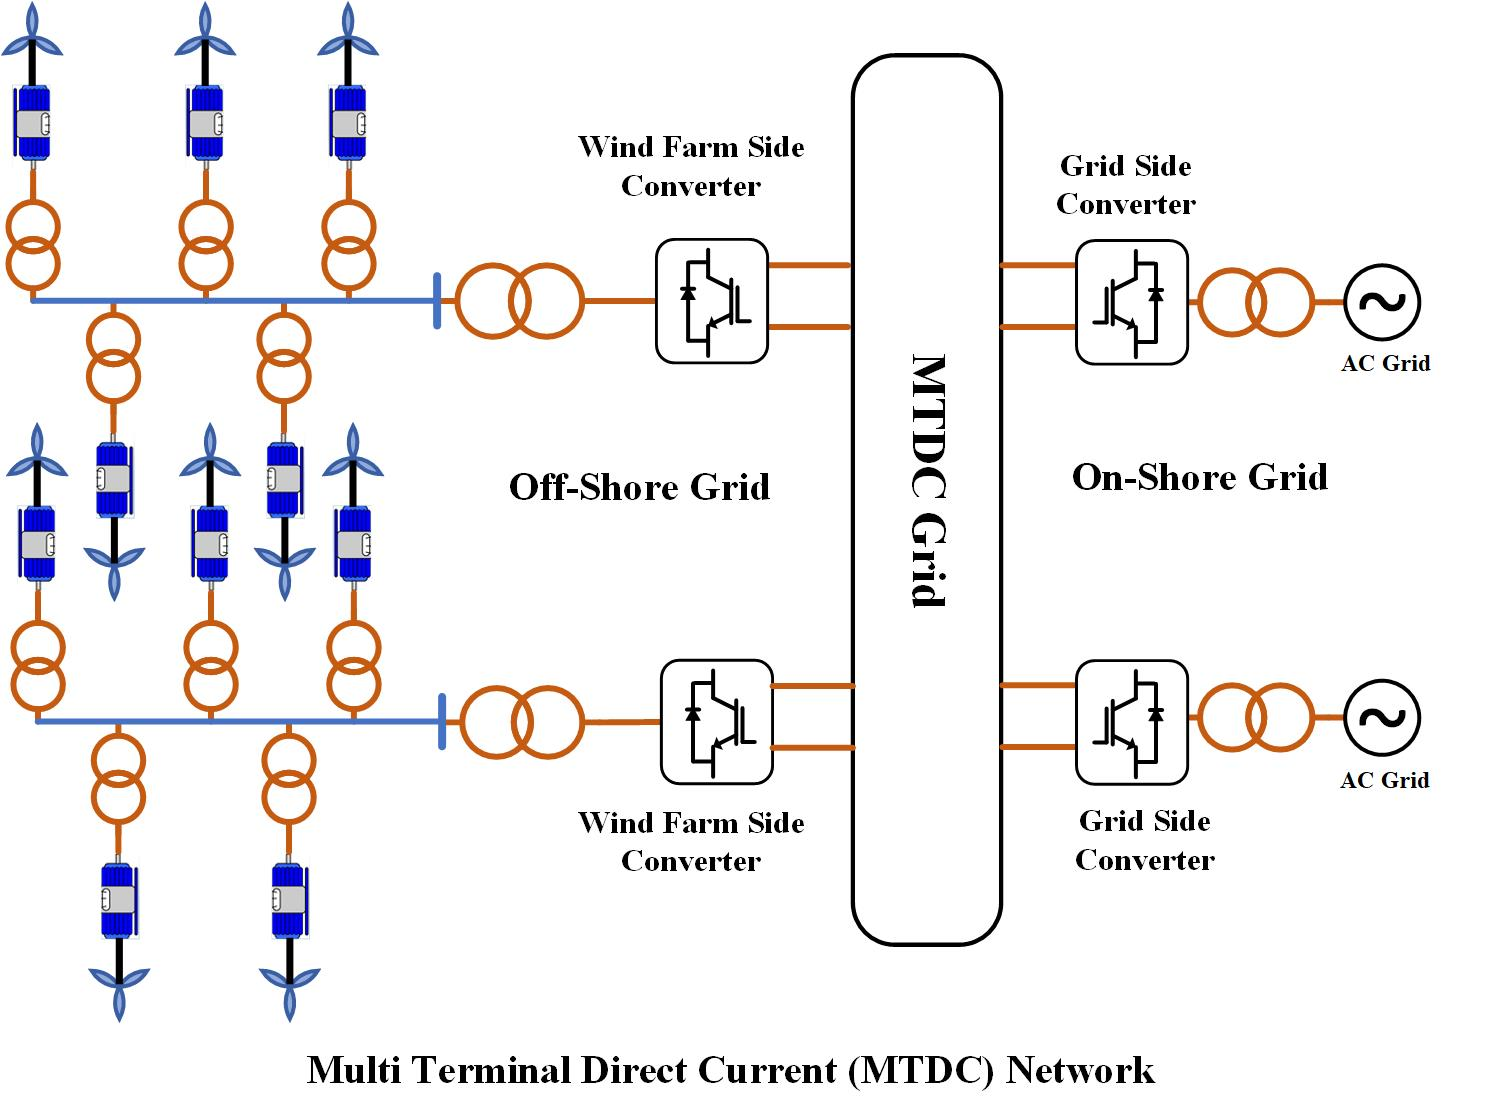
\includegraphics[width=3.3in]{Figures/singh16.png }}
\caption{Multi Terminal Direct Current (MTDC) Network.}
\label{MTDC}
\end{figure}



\begin{table*}[htbp]
\caption{HVDC Offshore Connection Topologies Comparison}
\renewcommand{\arrayrulewidth}{1.2pt} % Increase border thickness
\arrayrulecolor{black}
\renewcommand{\arraystretch}{1.3} % Adjust row height for better readability
\footnotesize % Use small font to ensure fitting within page width
\label{connection}
\centering
\begin{tabular}{|>{\raggedright\arraybackslash}p{3.0cm}|
                >{\centering\arraybackslash}p{3cm}|
                >{\centering\arraybackslash}p{2.5cm}|
                >{\centering\arraybackslash}p{1.2cm}|
                >{\centering\arraybackslash}p{1.2cm}|
                >{\centering\arraybackslash}p{0.7cm}|
                >{\centering\arraybackslash}p{1.3cm}|}
\hline
\makecell{\textbf{HVDC Offshore} \\ \textbf{Connection Topologies}} & \textbf{Advantages} & \textbf{Limitations} & \textbf{Feasibility} & \textbf{Reliability} & \textbf{Cost} & \textbf{Complexity} \\ 
\hline

\textbf{Parallel AC Collection System with HVDC Transmission} \cite{rodriguez2018control} & 
\begin{tabular}[]{@{}l@{}}$-$ Higher voltage/power \\ \hspace{8pt}transmission \\ $-$ Longer distances from \\ \hspace{8pt}shore\end{tabular} & 
\begin{tabular}[c]{@{}l@{}}$-$ Reactive power \\ \hspace{8pt}compensation \\ $-$ Lower reliability\end{tabular} & 
***** & *** & *** & ** \\ 
\hline

\textbf{Mesh-Connected AC Collection System with HVDC Transmission} \cite{pierri2017challenges} & 
\begin{tabular}[]{@{}l@{}}$-$ Enhanced system \\ \hspace{8pt}reliability \\ $-$ Improved redundancy\end{tabular} & 
\begin{tabular}[]{@{}l@{}}$-$ Infrastructure cost \\ $-$ Complex structure\end{tabular} & 
**** & **** & **** & **** \\ 
\hline

\textbf{Multi-Terminal DC Collection Grid with Mesh HVDC Transmission} \cite{rodriguez2017multi} & 
\begin{tabular}[]{@{}l@{}} $-$ Higher reliability; \\ \hspace{8pt}continued power transfer \\ \hspace{6pt} under cable failure\end{tabular} & 
\begin{tabular}[]{@{}l@{}}$-$ Infrastructure cost \\ $-$ Complex\end{tabular} & 
**** & ***** & ***** & **** \\ 
\hline

\textbf{Parallel DC Collection with Medium-Frequency Transformer Embedded HVDC Transmission} \cite{wei2016medium} & 
\begin{tabular}[]{@{}l@{}}$-$ Reduced offshore \\ \hspace{8pt}converter station \\ \hspace{8pt}footprint \& weight\end{tabular} & 
\begin{tabular}[]{@{}l@{}}$-$ Initial cost \& \\\hspace{5pt} transformer \\\hspace{8pt}technology\end{tabular} & 
\begin{tabular}[]{@{}l@{}}** \\ Under\\ Research\end{tabular} & *** & **** & *** \\ 
\hline

\textbf{Series DC Collection System with HVDC Transmission} \cite{bahirat2012reliability,sun2021reliability} & 
\begin{tabular}[]{@{}l@{}}$-$ Reduced infrastructure \\ \hspace{8pt}requirements \\ $-$ Elimination of offshore \\ \hspace{8pt}substations\end{tabular} & 
\begin{tabular}[]{@{}l@{}}$-$ Voltage maintenance \\ $-$ Reliability concerns\end{tabular} & 
\begin{tabular}[]{@{}l@{}}** \\ Under \\ Research\end{tabular} & ** & *** & *** \\ 
\hline

\end{tabular}
\end{table*}





Table \ref{connection} compares potential HVDC offshore connection topologies, assessing their advantages, limitations, feasibility, reliability, cost, and complexity to comprehensively understand the trade-offs involved and their suitability for offshore wind integration.



\subsection{\textbf{Economic Analysis for Connection Architecture}}
Economic analysis of connection architectures is critical for optimizing the cost-effectiveness of OWFs, as it directly impacts both capital expenditures (e.g., cabling and substations) and operational costs (e.g., transmission losses and maintenance). For a 500 MW reference wind farm comprising 50 turbines (10 MW each) spaced 1,000 meters apart, this study evaluates inter-array cabling layouts: radial, ring, branched, star, and mesh, as depicted in Fig. \ref{Collection_architecture.}. Such analyses are essential to identify configurations that minimize energy losses and infrastructure costs, thus improving the overall economic viability of OWFs \cite{stamatiou2010techno,van2010economic}.


\begin{table*}[htbp]
\renewcommand{\arrayrulewidth}{1.1pt} % Increase border thickness
\arrayrulecolor{black}

\renewcommand{\arraystretch}{1.2} % Increase row height for better readability
\small
\centering
\caption{Cost of Cable for Collection and Transmission Architecture}
\label{CablesUsed}

\begin{tabular}{|
p{1.4cm}<{\raggedright\arraybackslash} | 
p{1.0cm}<{\centering \arraybackslash} |
p{1.8cm}<{\centering\arraybackslash} |
p{2.4cm}<{\centering\arraybackslash} |
p{1.9cm}<{\centering\arraybackslash} |
p{1.2cm}<{\centering\arraybackslash} |
p{4cm}<{\centering\arraybackslash}|}
\hline
\textbf{Cable} & 
\textbf{Type} & 
\shortstack{\textbf{Voltage (kV)}} & 
\shortstack{\textbf{Diameter (mm$^2$)}} & 
\shortstack{\textbf{Ampere (A)} } & 
{$\mathbf{m\Omega}/\mathbf{km}$} & 
{\textbf{Transmission Loss} ($\text{kW}/\text{km}$)} \\ \hline
\textbf{Low} & AC & 110 & 1000 & 1283 & $16.8$ & $27.65$ \\ \hline
\textbf{Medium} & AC & 220 & 1600 & 1644 & $10.5$ & $28.37$ \\ \hline
\textbf{High} & AC & 500 & 800 & 1192 & $21$ & $29.84$ \\ \hline
\textbf{1} & DC & 150 & 1200 & 1375 & $14$ & $26.47$ \\ \hline
\textbf{2} & DC & 200 & 1600 & 1640 & $10.5$ & $28.24$ \\ \hline
\textbf{3} & DC & 250 & 1200 & 1375 & $14$ & $26.46$ \\ \hline
\textbf{4} & DC & 250 & 2500 & 2145 & $6.72$ & $30.92$ \\ \hline
\textbf{5} & DC & 320 & 800 & 1095 & $21$ & $25.18$ \\ \hline
\textbf{6} & DC & 320 & 2500 & 2145 & $6.72$ & $30.92$ \\ \hline
\end{tabular} % Close tabular here

\end{table*}


Each layout presents unique connectivity patterns that impact redundancy, reliability, and overall cost. The economic cost of the architecture is primarily determined by the chosen cable, which, in turn, is selected based on the required current-carrying capacity. This capacity is influenced by the total power transmission needs and the voltage rating of the wind turbine's grid-side converter. Within the selected architecture, the configuration and number of wind turbines in a string define each string's total power transmission capacity. It is also essential to incorporate a safety margin for the cable's current-carrying capacity to accommodate potential fault currents. Three distinct AC cable types and six DC cable types have been selected for a streamlined comparison of the different architectures, as presented in Table \ref{CablesUsed}. These cable types are utilized across both collection and transmission architectures \cite{meng2021comparative}. Copper serves as the conductor material in the cores of subsea cables, and consequently the cable resistance per kilometer is determined based on the resistivity of copper (standard resistivities of 1.68x$10^\text{-8}$ $\Omega$ m at $20^\circ\text{C}$) \cite{cullinane2022subsea}.

\begin{figure}[htbp]
\centerline{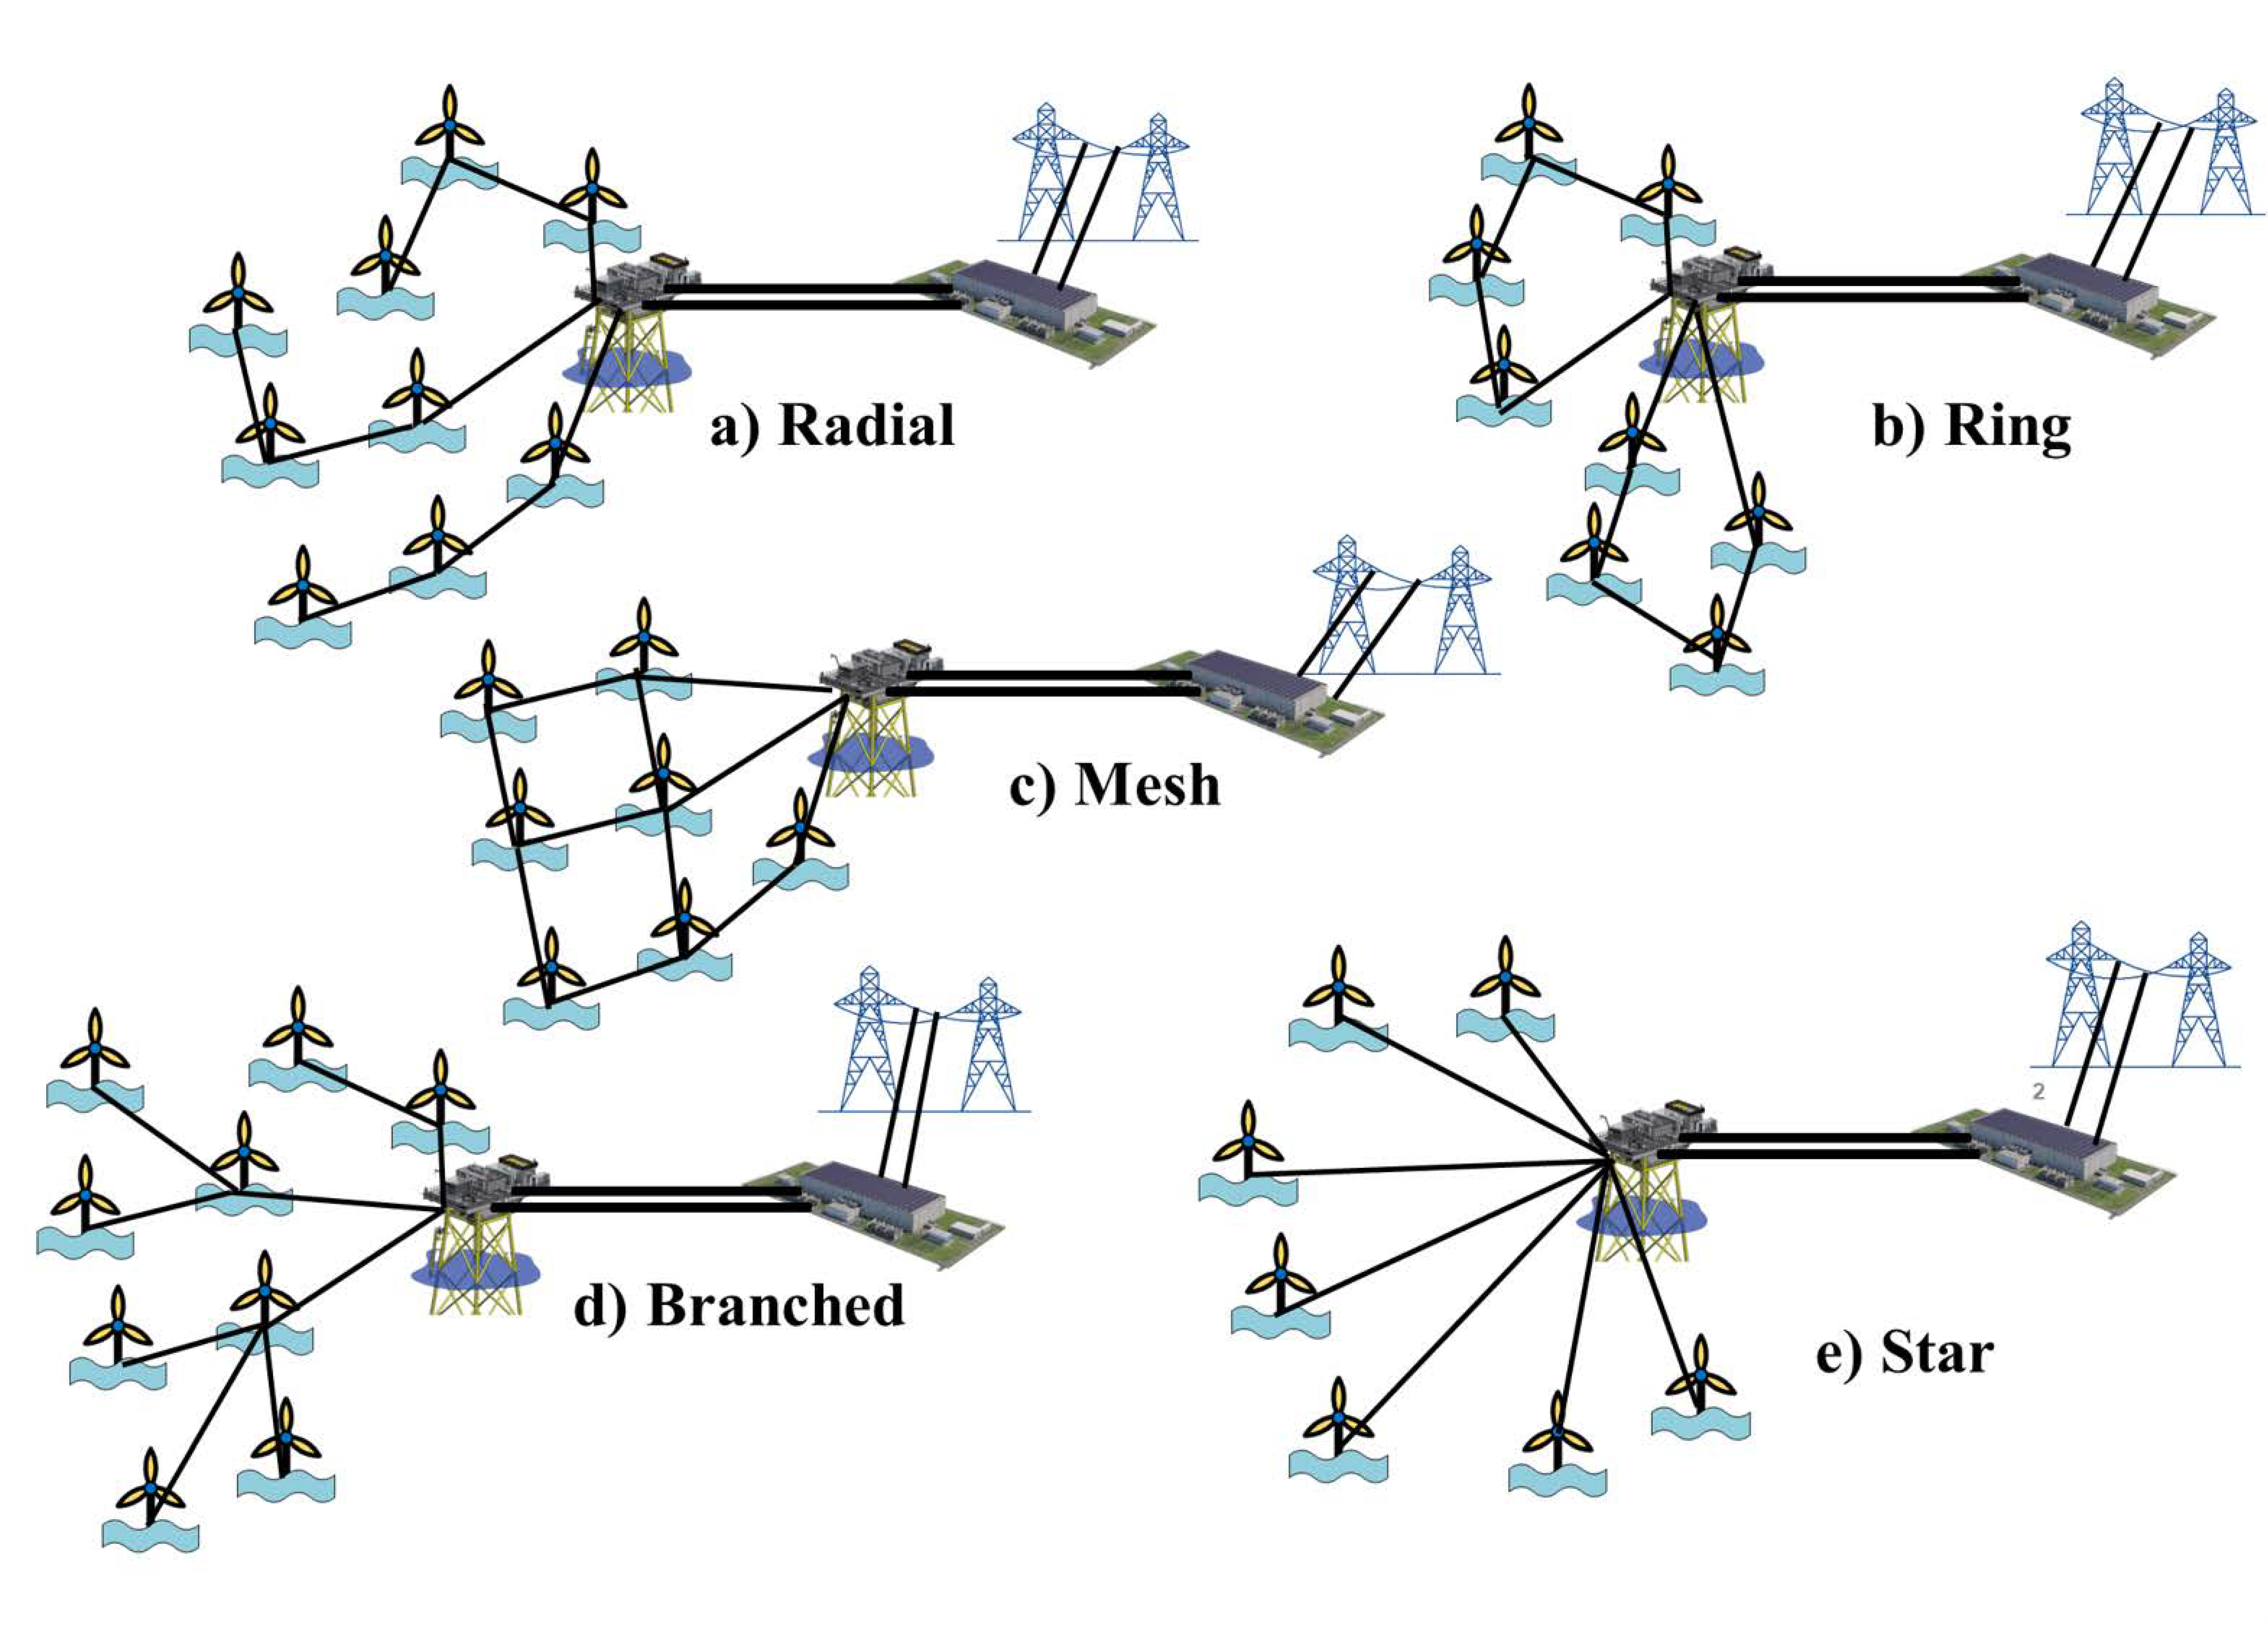
\includegraphics[width=3.3in]{Figures/singh17.png}}
\caption{Collection Architecture Techno-Economic Analysis.}
\label{Collection_architecture.}
\end{figure}


\begin{figure}[htbp]
\centerline{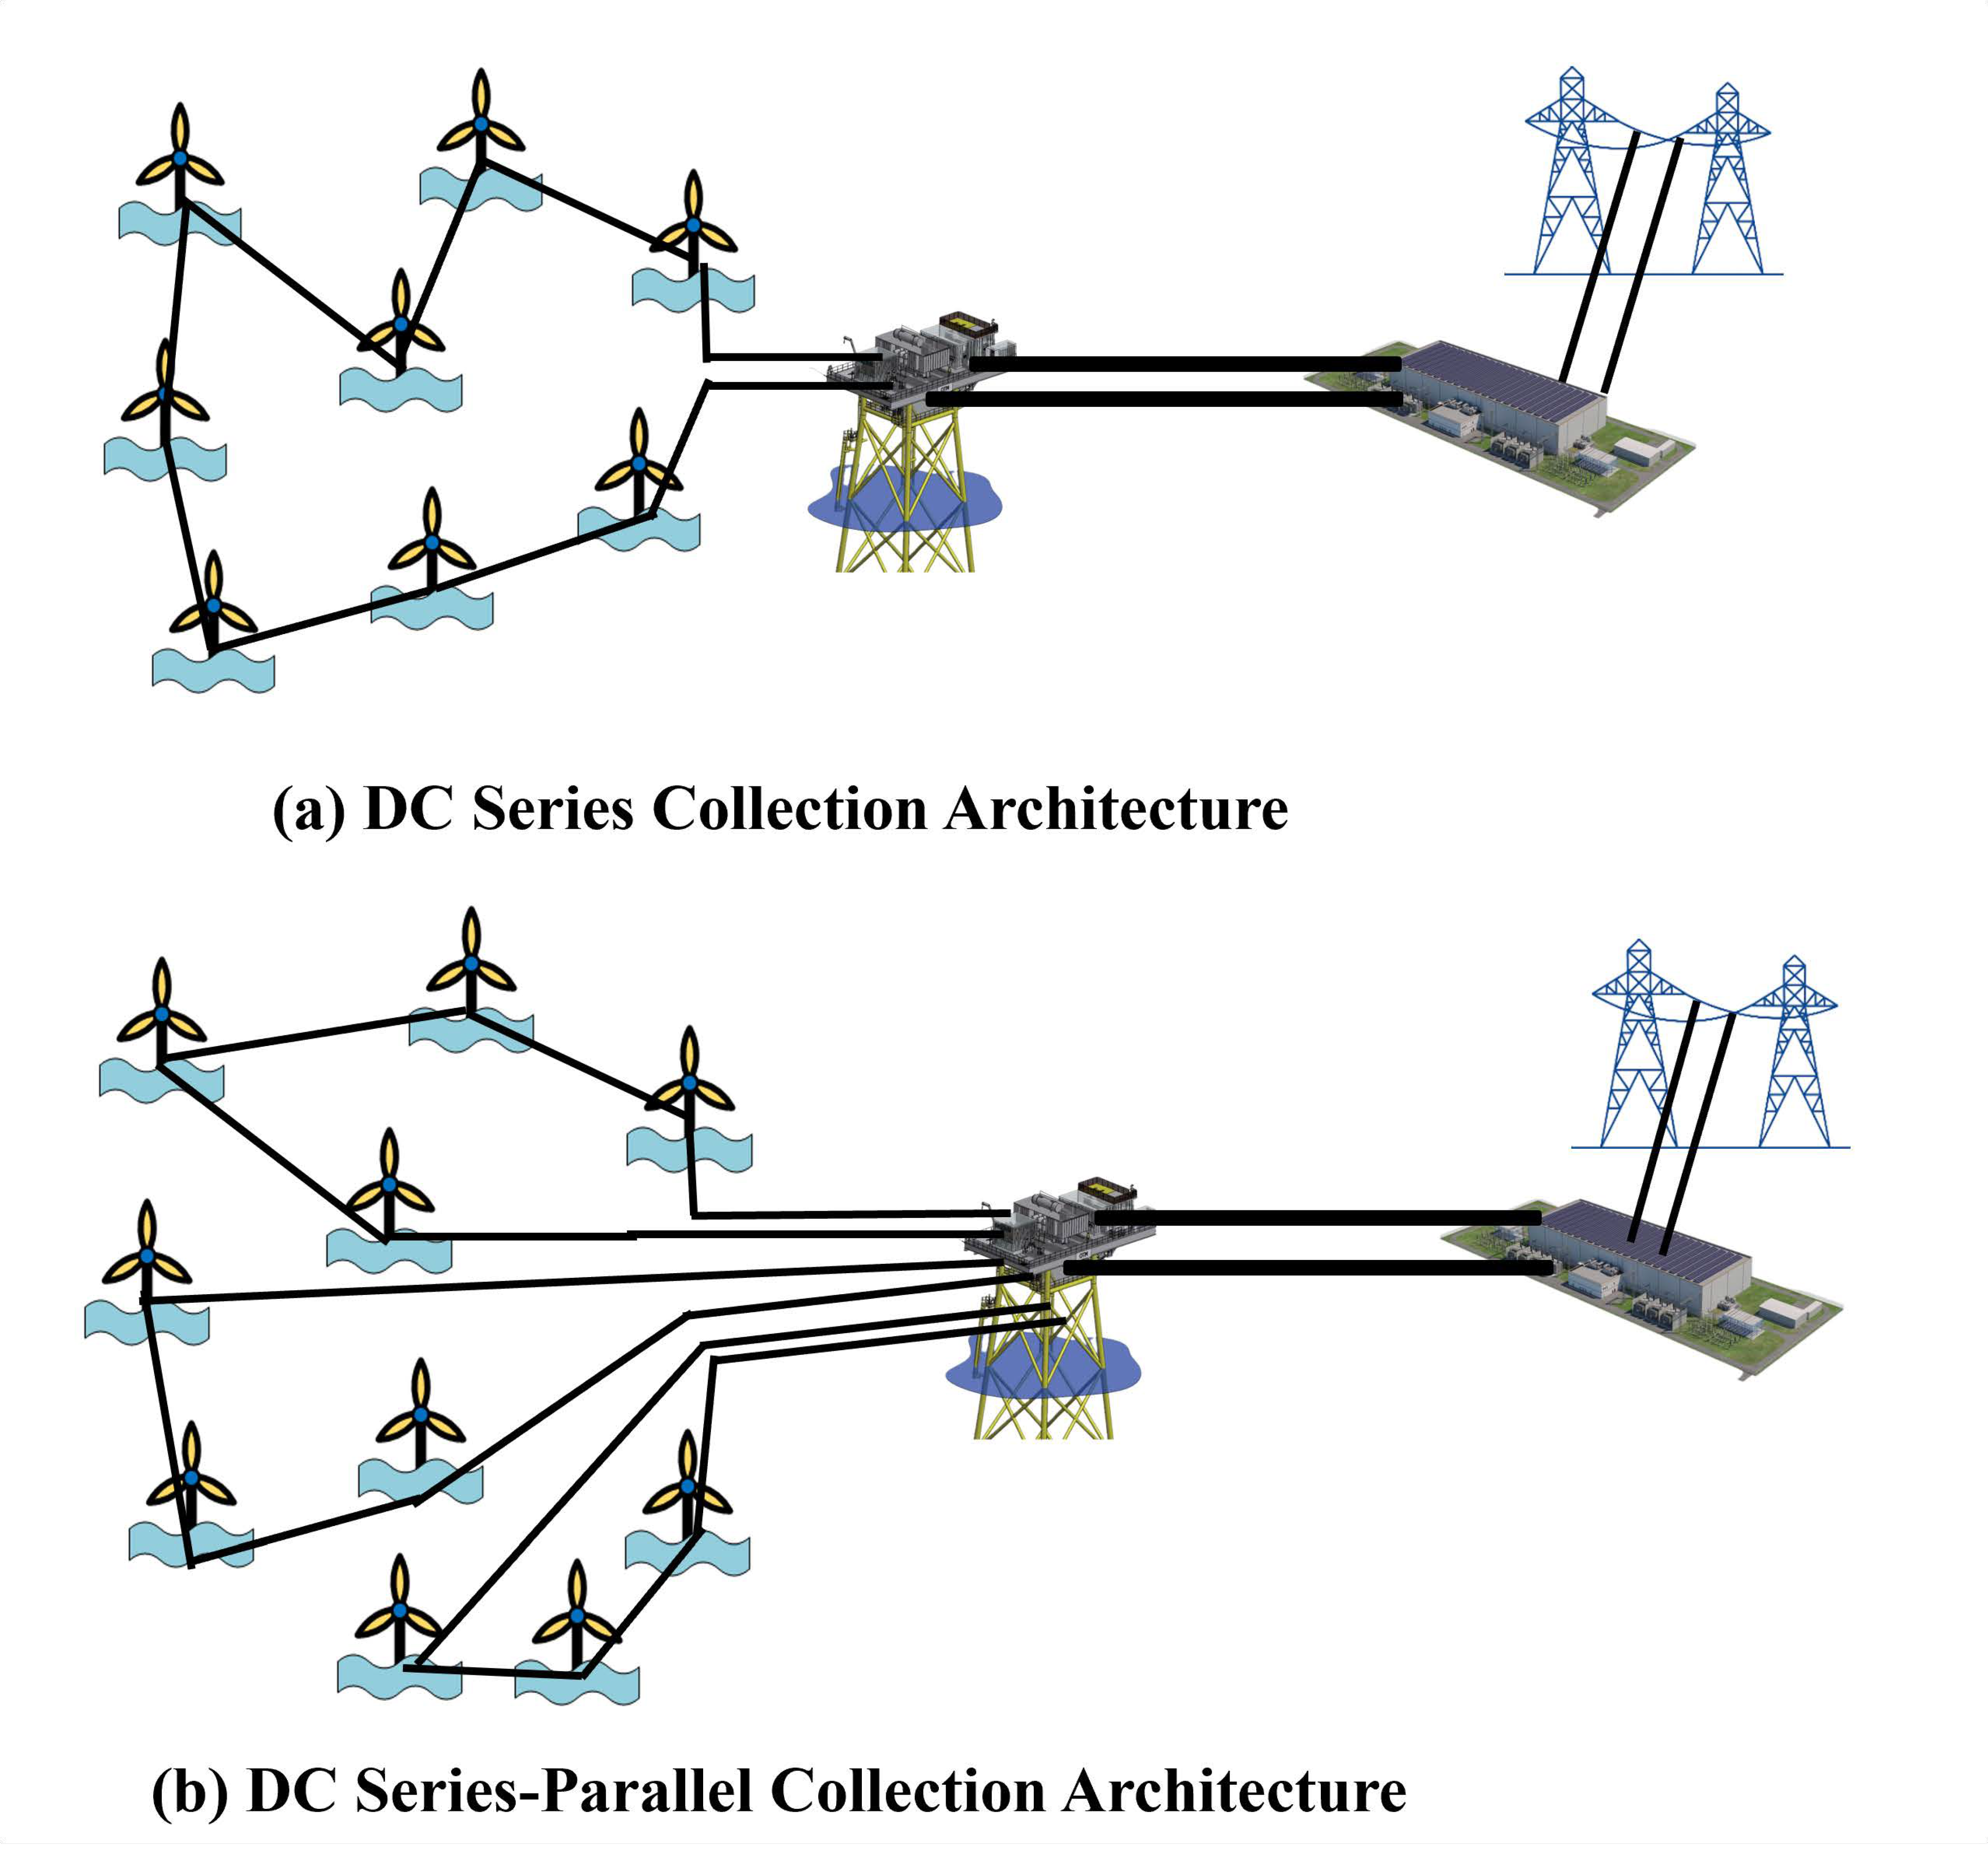
\includegraphics[width=3in]{Figures/singh18.png}}
\caption{DC Series Collection Architecture Techno-Economic Analysis.}
\label{DC_series_technoCollection_architecture}
\end{figure}


Table \ref{CollectionArchitectureTable} presents a comprehensive analysis of inter-array cable lengths, transmission losses, and reliability for different collection architectures. This includes details on power, current, and cable costs, providing an evaluation of the infrastructure and financial requirements for each architecture. The total length of each architecture is estimated by considering its complexity and redundancy, providing insights into how various architectural choices influence the overall cost.

The radial architecture connects wind turbines in series, with 10 strings of 5 turbines each, resulting in a total cable length of approximately 50 km and transmitting 50 MW of power per string. The ring architecture enhances connectivity by combining two radial strings with an additional 1 km cable, forming a ring with a total cable length of 55 km and transmitting 100 MW of power per ring. The branched architecture consists of 10 branches, each 5 km long, with 5 turbines per branch, totaling 50 km of cable and transmitting 50 MW of power per branch. In the star architecture, each turbine is directly connected to a central substation, averaging 2 km of cable per turbine, with a total cable length of 100 km and supporting 10 MW of power per turbine for reliable transmission. The mesh architecture interconnects each turbine to two or three neighbors, forming a network with an estimated total cable length of 120 km, capable of transmitting 50 MW of power while offering enhanced redundancy and reliability.

The analysis reveals that mesh architecture offers the highest reliability due to multiple power dispatch pathways, albeit at a higher cost. In contrast, ring architecture provides a balanced option with two dispatch pathways, ensuring reliability and cost efficiency. An additional analysis of the DC series, DC series-parallel (Fig. \ref{DC_series_technoCollection_architecture}), and DC parallel architectures (comparable to the radial configuration shown in Fig. \ref{Collection_architecture.}(a)) is conducted and summarized in Table \ref{DC_series_table}. The results indicate that the parallel architecture offers better reliability due to its inherent redundancy; however, this advantage comes at the cost of increased expenses and higher power losses.



\begin{table*}[htbp]
\renewcommand{\arrayrulewidth}{1.1pt} % Increase border thickness
\arrayrulecolor{black}
\renewcommand{\arraystretch}{1.4} % Increase row height for better readability
\small
\centering
\caption{Cost of Cable for AC Collection Architecture}
\label{CollectionArchitectureTable}
\begin{tabular}{|
p{2.0cm}<{\raggedright\arraybackslash} |
p{2.1cm}<{\centering\arraybackslash} |
p{1.5cm}<{\centering\arraybackslash} |
p{1.5cm}<{\centering\arraybackslash} |
p{1.5cm}<{\centering\arraybackslash} |
p{1.5cm}<{\centering\arraybackslash} |
p{1.5cm}<{\centering\arraybackslash} |
p{1.5cm}<{\centering\arraybackslash} |}
\hline
\textbf{Architecture} & 
\begin{tabular}[c]{@{}c@{}}\textbf{Total Estimated} \\ \textbf{Inter-Array} \\ \textbf{Cable} \\ \textbf{Length} \textbf{(km)}\end{tabular} & 
\begin{tabular}[c]{@{}c@{}}\textbf{Cable} \\ \textbf{Used}\end{tabular} & 
\begin{tabular}[c]{@{}c@{}}\textbf{Total} \\ \textbf{Power per} \\ \textbf{String} \\ \textbf{(MW)}\end{tabular} & 
\begin{tabular}[c]{@{}c@{}}\textbf{Cable} \\ \textbf{Cost} \\ \textbf{(k\$ / km)}\end{tabular} & 
\begin{tabular}[c]{@{}c@{}}\textbf{Calculated} \\ \textbf{Cable} \\ \textbf{Cost (M\$)}\end{tabular} & 
\begin{tabular}[c]{@{}c@{}}\textbf{Calculated} \\ \textbf{Power} \\ \textbf{Loss (MW)}\end{tabular} & 
\textbf{Reliability} \\ \hline
 & 50 & Low & 50 & 1070 & 53.5 & 1.38 & * \\ \cline{2-8}
 & 50 & Medium & 50 & 1926 & 96.3 & 1.41 & * \\ \cline{2-8}
\multirow{-3}{*}{\textbf{Radial}} & 50 & High & 50 & 2208 & 110.4 & 1.49 & * \\ \hline
 & 55 & Low & 100 & 1070 & 58.9 & 1.52 & *** \\ \cline{2-8}
 & 55 & Medium & 100 & 1926 & 105.9 & 1.56 & *** \\ \cline{2-8}
\multirow{-3}{*}{\textbf{Ring}} & 55 & High & 100 & 2208 & 121.44 & 1.64 & *** \\ \hline
 & 50 & Low & 50 & 1070 & 53.5 & 1.38 & ** \\ \cline{2-8}
 & 50 & Medium & 50 & 1926 & 96.3 & 1.42 & ** \\ \cline{2-8}
\multirow{-3}{*}{\textbf{Branched}} & 50 & High & 50 & 2208 & 110.4 & 1.49 & ** \\ \hline
 & 100 & Low & 10 & 1070 & 107 & 2.76 & ** \\ \cline{2-8}
 & 100 & Medium & 10 & 1926 & 192.6 & 2.82 & ** \\ \cline{2-8}
\multirow{-3}{*}{\textbf{Star}} & 100 & High & 10 & 2208 & 220.8 & 2.98 & ** \\ \hline
 & 120 & Low & 50 & 1070 & 128.4 & 3.32 & **** \\ \cline{2-8}
 & 120 & Medium & 50 & 1926 & 231.1 & 3.41 & **** \\ \cline{2-8}
\multirow{-3}{*}{\textbf{Mesh}} & 120 & High & 50 & 2208 & 128.4 & 3.58 & **** \\ \hline
\end{tabular}

\end{table*}


A similar analysis is conducted for transmission architectures, including single point-to-point, multi-terminal point-to-point, multi-terminal radial, and multi-terminal mesh configurations, as illustrated in Fig. \ref{Transmission-a.}, Fig. \ref{Transmission-b.}, Fig. \ref{Transmission-c.}, and Fig. \ref{Transmission-d.}. DC export cables, selected based on their power and current-carrying capacity from Table \ref{CablesUsed}, are analyzed in Table \ref{TransmissionArchitectureTable}. This detailed techno-economic analysis compares six export cables for each transmission architecture, concluding that the multi-terminal mesh architecture provides the highest reliability, though at a slightly higher cost, while the multi-terminal radial architecture offers better reliability at a favorable cost.

\begin{table*}[htbp]
\caption{Cost of Cable for DC Series, Parallel, and Series-Parallel Collection Architecture}
\renewcommand{\arrayrulewidth}{1.1pt} % Increase border thickness
\arrayrulecolor{black}
\renewcommand{\arraystretch}{1.3} % Increase row height for better readability
\small
\centering
\label{DC_series_table}
\begin{tabular}{|
p{2.4cm}<{\raggedright\arraybackslash} |
p{2.2cm}<{\centering\arraybackslash} |
p{1.8cm}<{\centering\arraybackslash} |
p{1.5cm}<{\centering\arraybackslash} |
p{1.5cm}<{\centering\arraybackslash} |
p{2.0cm}<{\centering\arraybackslash} |
p{1.5cm}<{\centering\arraybackslash} |}
\hline
\textbf{Architecture} & \makecell[c]{\bfseries Estimated \\ \textbf{Cable}\\ \textbf{Length (km)}} & \makecell[c]{\bfseries Cable \textbf{Used}} & \makecell[c]{\bfseries Cable Cost \\ \textbf{k\$ per km}} & \makecell[c]{\bfseries Calculated \\ \textbf{Cable Cost} \\ \hspace{8pt}\textbf{(M\$)}} & \makecell[c]{\bfseries Calculated \\ \textbf{Power}\\ \textbf{Loss (MW)}} & \textbf{Reliability} \\ \hline
\textbf{Series}                & 55                                   & 1                   & 936                                & 51.48                                & 1.455                               & *  \\ \hline
\textbf{Parallel}              & 120                                  & 1                   & 936                                & 112.32                               & 3.17                                & ***  \\ \hline
\textbf{Series-Parallel}       & 65                                   & 1                   & 936                                & 60.84                                & 1.72                                & **  \\ \hline
\end{tabular}
\end{table*}

\begin{table*}[htbp]
\caption{Cost of Cable for DC Transmission Architecture}
\renewcommand{\arrayrulewidth}{1.1pt} % Increase border thickness
\arrayrulecolor{black}
\renewcommand{\arraystretch}{1.3} % Increase row height for better readability
\small
\label{TransmissionArchitectureTable}
\centering
\begin{tabular}{|
p{4.0cm}<{\raggedright\arraybackslash}|
p{1.8cm}<{\centering\arraybackslash}|
p{1.1cm}<{\centering\arraybackslash}|
p{0.9cm}<{\centering\arraybackslash}|
p{1.5cm}<{\centering\arraybackslash}|
p{1.5cm}<{\centering\arraybackslash}|
p{1.6cm}<{\centering\arraybackslash}|
p{1.2cm}<{\centering\arraybackslash}|}
\hline
\textbf{Architecture} &
\makecell[c]{\textbf{Estimated} \\ \textbf{Cable}\\ \textbf{Length (km)}} &
\textbf{Cable Used} &
\textbf{Sets} &
\makecell[c]{\textbf{Cable Cost} \\ \textbf{(k\$ per km)}} &
\makecell[c]{\textbf{Calculated} \\ \textbf{Cable}\\ \textbf{Cost (M\$)}} &
\makecell[c]{\textbf{Calculated}\\ \textbf{ Power} \\ \textbf{Loss (kW)}} &
\textbf{Reliability} \\ \hline

\multirow{1}{*}{} & 100 & 1 & 3 & 936 & 280.8 & 7,941 & * \\ \cline{2-8}
& 100 & 2 & 2 & 1,183 & 236.6 & 5,648 & * \\ \cline{2-8}
& 100 & 3 & 2 & 1,136 & 227.2 & 5,294 & * \\ \cline{2-8}
{ \textbf{Single Point to Point}} & 100 & 4 & 1 & 1,614 & 161.4 & 3,093 & * \\ \cline{2-8}
& 100 & 5 & 2 & 1,130 & 226.0 & 5,036 & * \\ \cline{2-8}
& 100 & 6 & 1 & 1,755 & 175.5 & 3,092 & * \\ \hline

\multirow{1}{*} & 300 & 1 & 1 & 936 & 280.8 & 7,941 & ** \\ \cline{2-8}
& 300 & 2 & 1 & 1,183 & 354.9 & 8,472 & ** \\ \cline{2-8}
& 300 & 3 & 1 & 1,136 & 340.8 & 7,941 & ** \\ \cline{2-8}
{\textbf{Multi-Terminal Point to Point}}& 300 & 4 & 1 & 1,614 & 484.2 & 9,278 & ** \\ \cline{2-8}
& 300 & 5 & 1 & 1,130 & 339.0 & 7,554 & ** \\ \cline{2-8}
& 300 & 6 & 1 & 1,755 & 526.5 & 9,276 & ** \\ \hline

\multirow{1}{*} & 203 & 1 & 3 & 936 & 570.0 & 16,119 & *** \\ \cline{2-8}
& 203 & 2 & 2 & 1,183 & 480.3 & 11,466 & *** \\ \cline{2-8}
& 203 & 3 & 2 & 1,136 & 461.2 & 10,746 & *** \\ \cline{2-8}
{\textbf{Multi-Terminal Radial}}& 203 & 4 & 1 & 1,614 & 327.6 & 6,278 & *** \\ \cline{2-8}
& 203 & 5 & 2 & 1,130 & 458.8 & 10,223 & *** \\ \cline{2-8}
& 203 & 6 & 1 & 1,755 & 356.3 & 6,277 & *** \\ \hline

\multirow{1}{*} & 206 & 1 & 3 & 936 & 578.4 & 16,358 & **** \\ \cline{2-8}
& 206 & 2 & 2 & 1,183 & 487.4 & 11,635 & **** \\ \cline{2-8}
& 206 & 3 & 2 & 1,136 & 468.0 & 10,905 & **** \\ \cline{2-8}
{\textbf{Multi-Terminal Mesh}}& 206 & 4 & 1 & 1,614 & 332.5 & 6,370 & **** \\ \cline{2-8}
& 206 & 5 & 2 & 1,130 & 465.6 & 10,374 & **** \\ \cline{2-8}
& 206 & 6 & 1 & 1,755 & 361.5 & 6,369 & **** \\ \hline

\end{tabular} 

\end{table*}




\begin{figure}[htbp]
\centerline{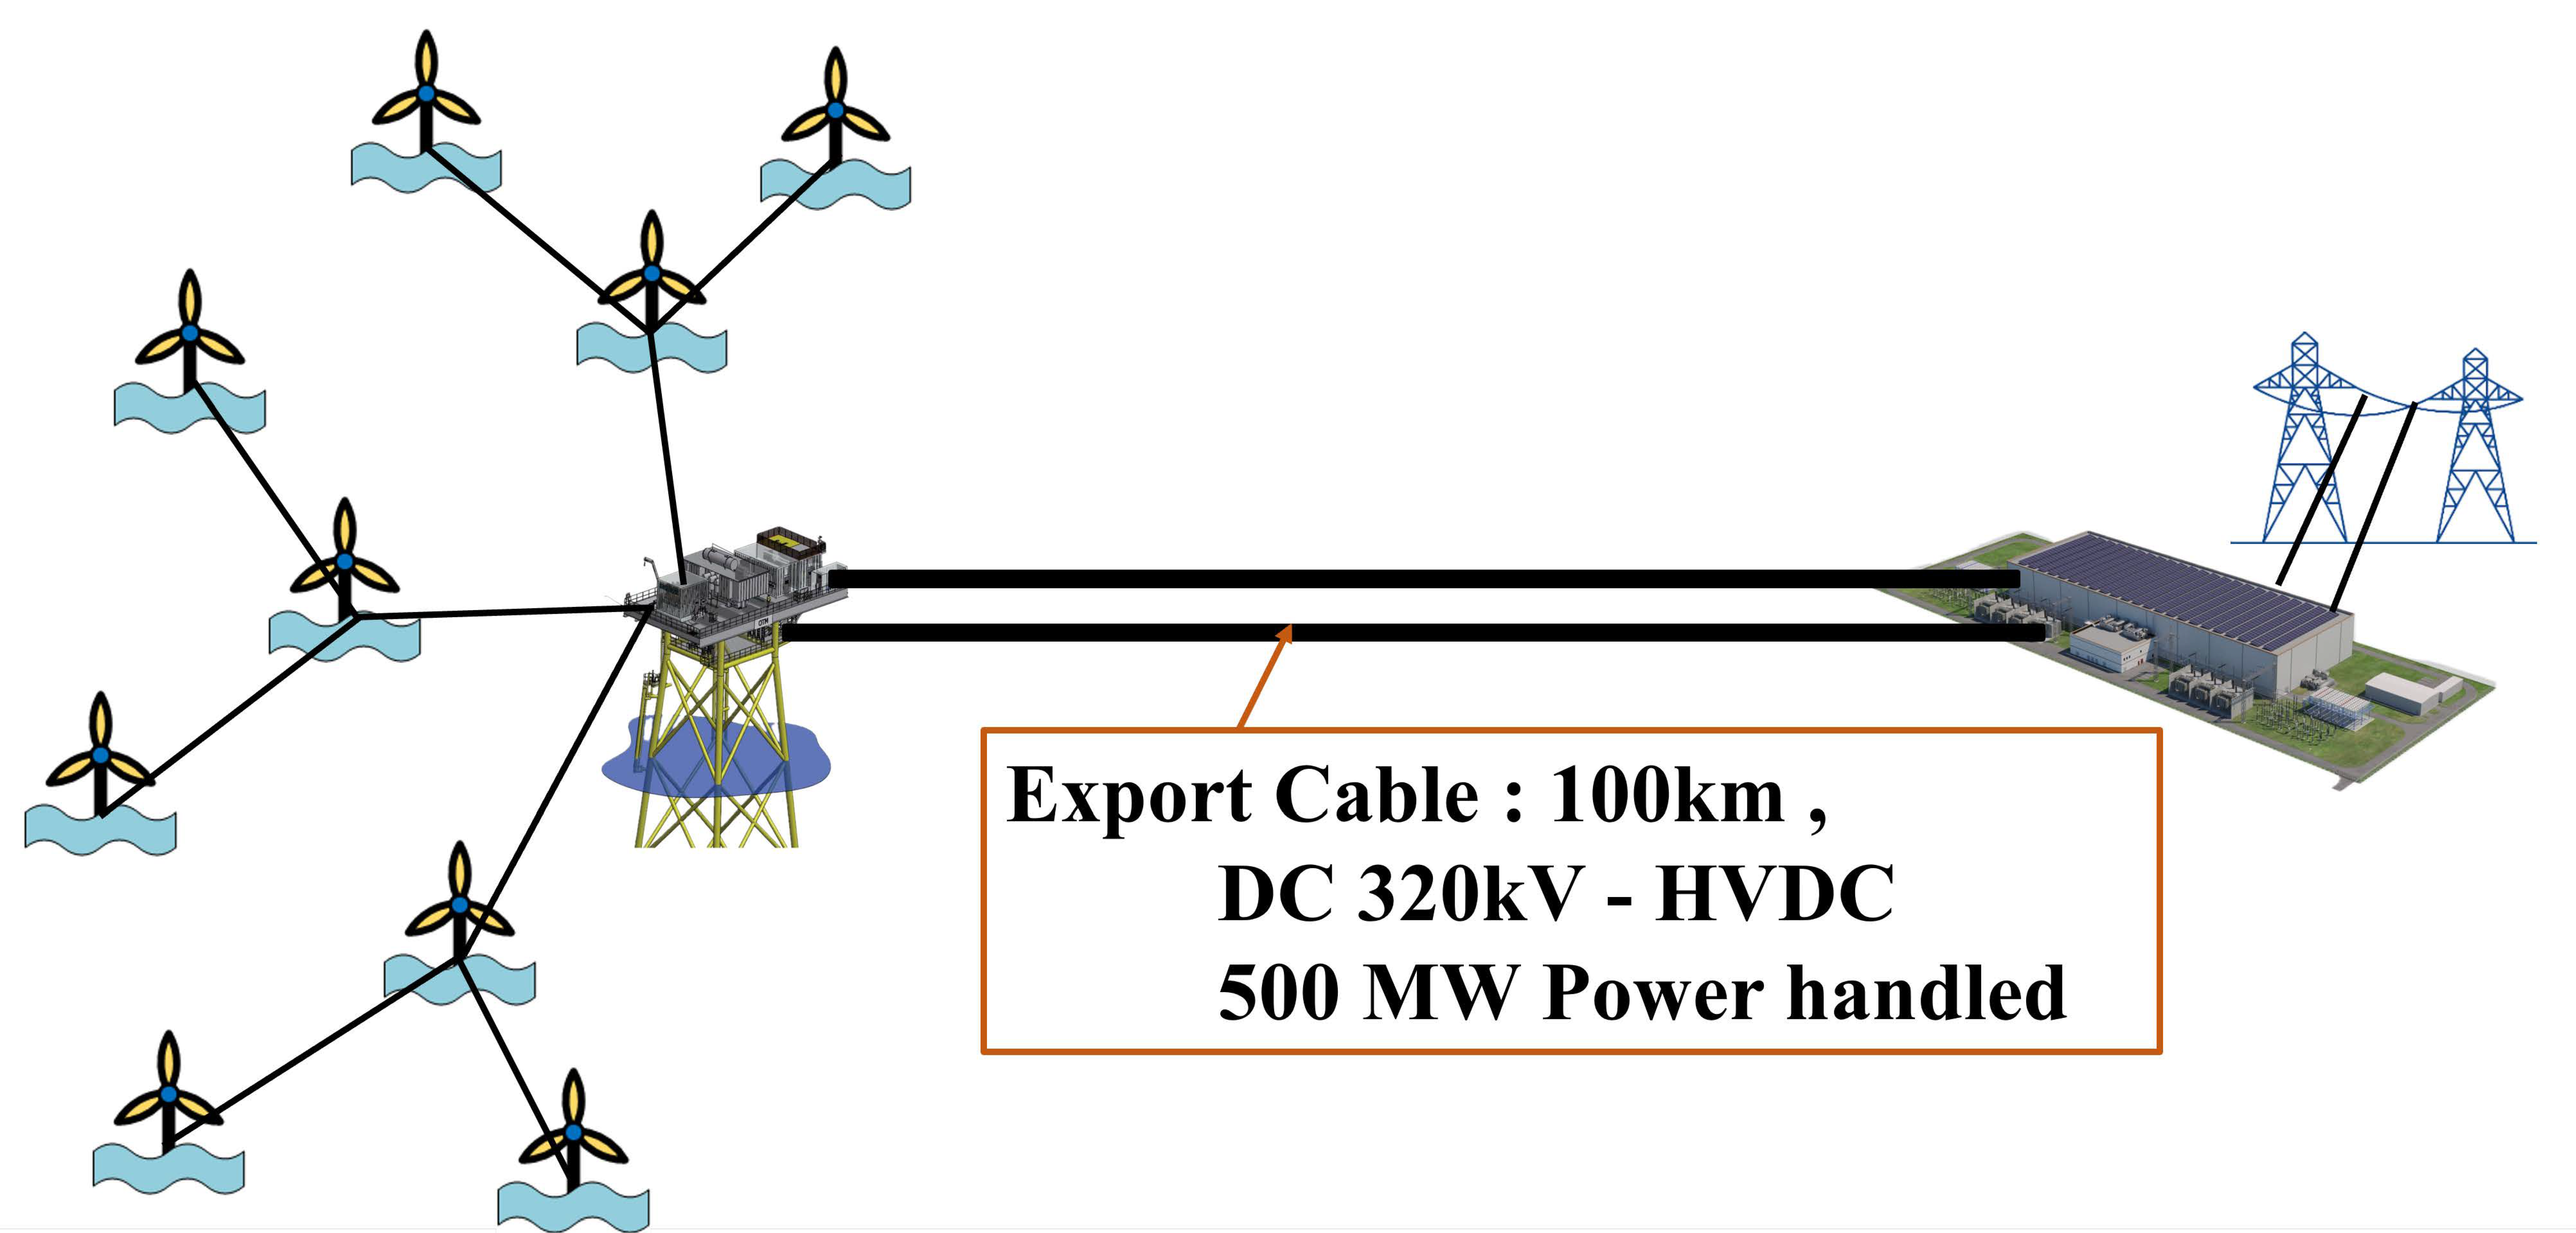
\includegraphics[width=3.2in]{Figures/singh19.png}}
\caption{Single Point Transmission Architecture.}
\label{Transmission-a.}
\end{figure}

\begin{figure}[htbp]
\centerline{\includegraphics[width=3.3in]{Figures/singh20.png}}
\caption{Multi-Terminal Grid Design Point to Point Transmission Architecture.} 
\label{Transmission-b.}
\end{figure}


\begin{figure}[htbp]
\centerline{\includegraphics[width=3.2in]{Figures/singh21.png}}
\caption{Multi-Terminal Grid Design Radial Transmission Architecture.} 
\label{Transmission-c.}
\end{figure}

\begin{figure}[htbp]
\centerline{\includegraphics[width=3in]{Figures/singh22.png}}
\caption{Multi-Terminal Grid Design Meshed Transmission Architecture.}
\label{Transmission-d.}
\end{figure}



\section{\textbf{Power Converter Topologies}}

Power electronic converters play a pivotal role in converting power from one electrical form to another, maintaining the stability and quality of power, and ensuring grid compatibility. The technology used for these converters determines the overall efficiency, the response time to grid disturbances, and the performance of the system, making the selection of converter technology a significant step in the design of the HVDC transmission system \cite{inamdar2018converters}. Each converter technology provides unique characteristics and suitability for specific applications \cite{li2021review,amorim2020analysis}.

Criteria for selection depend on various factors such as collection architectures, transmission distance, capacity requirements, grid conditions, and cost considerations. The grid side converter is always DC/AC, but based on the output from the wind turbine (AC or DC), the wind turbine side converter can either be AC/DC or DC/DC \cite{biswas2021high,mitra2018hvdc,ryndzionek2020evolution}.
Fig. \ref{Converterclassification.} shows the classification of the power electronic converter used for collection and transmission architectures for HVDC applications in OWFs.

\begin{figure*}[htbp]
\centerline{
\includegraphics[width=6in]{Figures/singh23.png }}
\caption{Classification of Power Electronic Converters in HVDC in OWF.}
\label{Converterclassification.}
\end{figure*}

\subsection{\textbf{AC/DC Converters}}
AC/DC converters can be categorized based on the type of switches used into (i) Diode Rectifiers (DRs), (ii) Line-Commutated Converters (LCCs),(iii) Voltage Source Converters (VSCs), and (iv) Hybrid Converters.


DRs have applications in low (<1 kV) to medium Voltage (33-66 kV) systems collection and transmission, but they are generally not the preferred choice for HVDC transmission systems associated with OWFs \cite{cai2022offshore}. Due to the variable nature of wind power, the uncontrolled operation of DRs makes them unsuitable for such applications. Furthermore, DRs lack the ability to provide reactive power support, which is essential for maintaining voltage stability and ensuring grid compliance. Furthermore, they introduce significant harmonic distortions into the electrical system \cite{yang2022critical}.


LCC technology is a well-established solution for HVDC transmission, offering exceptional performance in long-distance, high-capacity power transfer and robust handling of short circuits \cite{oni2016review,flourentzou2009vsc,singh2022voltage}. However, it faces notable challenges, particularly in reactive power control. LCC requires external compensation devices, such as STATCOMs, due to limitations imposed by the inverter's extinction angle \cite{xue2016reactive}. Compared to the flexible, reactive power control of VSCs, the adaptability of LCC is limited \cite{oni2016review,buigues2017present,fein2013dual,yang2022critical}.

Furthermore, LCC-HVDC systems are not suitable for weak grids with SCR < 2 due to stability concerns and reliance on strong AC systems for commutation \cite{lu2017evaluation}. %\cite{vo2022stability}.
It is also sensitive to grid disturbances and generates significant harmonic distortions, necessitating complex filtering solutions. Additionally, LCC lacks bidirectional power flow flexibility and is hindered by its large size and weight, making it impractical for OWFs, where space optimization is critical \cite{ryndzionek2020evolution,blasco2012lcc}. These limitations highlight the need to carefully evaluate LCC's strengths and weaknesses when considering its application across diverse scenarios.

To overcome the challenges posed by LCC technology, the industry is increasingly shifting toward more advanced solutions such as VSCs, which utilize fully controllable transistors such as IGBTs \cite{flourentzou2009vsc}. VSCs offer bidirectional power flow control, enhance voltage stability through reactive power management, and provide black start capability, making them reliable for HVDC applications \cite{koondhar2023critical,zhang2022coordinated}. However, the adoption of VSCs has been relatively slow, in part due to the need for additional filters to manage the high voltage (dv/dt) and current (di/dt) slew-rates, which increases costs and complexity \cite{flourentzou2009vsc,jiang2018day}. To improve market penetration, VSC systems must address challenges such as switching losses and harmonic distortion \cite{buigues2017present,yang2022critical}. Nonetheless, their adaptability positions them well for future integration into OWFs \cite{oni2016review,xu2023amplitude}.

\begin{table*}[htbp]
\renewcommand{\arrayrulewidth}{1.1pt} % Border thickness
\arrayrulecolor{black}
\renewcommand{\arraystretch}{1.2} % Row height for better alignment
\renewcommand{\tabcolsep}{5pt}
\small
\caption{Comparative Analysis of AC/DC Converters for OSW HVDC}
\centering
\label{Comparative Analysis of Converter for OSW HVDC}
\begin{tabular}{|
>{\raggedright\arraybackslash}p{2.6cm}|
>{\raggedright\arraybackslash}p{2.9cm}|
>{\raggedright\arraybackslash}p{2.9cm}|
>{\raggedright\arraybackslash}p{2.9cm}|
>{\raggedright\arraybackslash}p{2.9cm}|}
\hline
\textbf{Converter Type} & 
\textbf{Line Commuted Converter} & 
\textbf{Voltage Source Converter} & 
\textbf{Modular Multilevel Converter} & 
\textbf{Alternate Arm Modular Converter} \\
\hline

% Losses
\textbf{Losses} & 
Low switching losses \cite{oni2016review} & 
High switching losses \cite{oni2016review, spahic2005offshore} &  
\textless{}1\% semiconductor losses \cite{debnath2014operation} & 
Lower than MMC and VSC \cite{merlin2013alternate} \\
\hline

% Commutation
\textbf{Commutation} & 
External commutation \cite{oni2016review} & 
Self-commutated & 
Self-commutated & 
Self-commutated \\
\hline

% Reactive Power Compensation
\textbf{Reactive Power Compensation} & 
Limited \cite{xue2016reactive, buigues2017present} & 
Flexible \cite{oni2016review} & 
Flexible modes \cite{yu2021bpa} & 
Offers compensation, enhancing stability \cite{merlin2013alternate} \\
\hline

% DC - Fault Tolerance
\textbf{DC - Fault Tolerance} & 
Withstands short circuits \cite{flourentzou2009vsc} & 
Vulnerable to line faults \cite{flourentzou2009vsc, soomro2022detailed} & 
Half-bridge SMs lack fault handling \cite{merlin2013alternate} & 
Strong fault tolerance \cite{wickramasinghe2018alternate, sun2021hybrid} \\
\hline

% Power Flow Direction
\textbf{Power Flow Direction} & 
DC polarity inversion \cite{oni2016review} & 
Bidirectional control \cite{spahic2005offshore} & 
Bidirectional \cite{yu2021bpa, sun2021hybrid} & 
Bidirectional \cite{sun2021hybrid} \\
\hline

% Suitability for OSW
\textbf{Suitability for OSW} & 
Suitable for long-distance transmission \cite{oni2016review} & 
Suitable for both medium voltage DC collection and HVDC transmission \cite{oni2016review, flourentzou2009vsc} & 
Most suitable for HVDC transmission \cite{li2019coordinated} & 
Potential alternative for HVDC transmission; still in development \cite{merlin2013alternate} \\
\hline

% EMI Challenges
\textbf{EMI Challenges} & 
Minimal \cite{flourentzou2009vsc} & 
Requires additional filters \cite{flourentzou2009vsc} & 
Continuous arm reduces EMI \cite{martinez2017modular} & 
Lower dv/dt; superior EMI performance \cite{sun2021hybrid} \\
\hline

% Footprint and Weight
\textbf{Footprint \& Weight} & 
Large volume and high weight \cite{oni2016review} & 
Smaller footprints \cite{bresesti2007hvdc} & 
Reduced footprint due to modular structure \cite{martinez2017modular} & 
Smaller footprint and reduced weight \cite{merlin2013alternate} \\
\hline

\end{tabular}
\end{table*}






The VSCs are classified as (i) Two-level, (ii) Three-level, and (iii) N-level (Multilevel), based on output voltage levels. Two-level VSCs switch between positive and negative DC voltage, making them simple and cost-effective for low voltage collection architectures but limited in HVDC transmission applications. Three-level VSCs like Neutral Point Clamped (NPC) and Active Neutral Point Clamped (ANPC) add a zero voltage level, offering lower harmonic distortion and better efficiency for medium voltage high-power systems \cite{beerten2014modeling}. N-level (Multilevel) VSCs, like Cascaded-H Bridge and Modular Multilevel Converter (MMC), generate multiple voltage levels, reducing harmonics and improving efficiency in high-voltage applications. MMCs are favored in offshore wind HVDC transmission systems for their higher efficiency, better control, superior harmonic performance, scalability, and better fault tolerance and reliability in high-voltage settings  \cite{zhong2020topology,chattopadhyay2019full,nami2019frequency}.




MMC is a promising technology for HVDC transmission, particularly in integrating OWFs \cite{inamdar2018converters}. Its modular design enables high voltage levels and low switching frequencies, reducing harmonics and electromagnetic interference (EMI) \cite{debnath2014operation}. MMC independently controls active and reactive power, improving grid stability \cite{zhou2022active,lin2023impact}. Modular redundancy bolsters fault tolerance, ensuring reliability in demanding HVDC conditions \cite{8259001}. Furthermore, MMC supports bidirectional power flow, which makes it ideal for dynamic energy systems \cite{li2019coordinated}. Although still in development, ongoing research on MMCs continues to focus on enhancing their reliability\cite{debnath2014operation,zhang2023optimal,zhou2023characteristic,li2019coordinated}.



Conventional MMC structures are modified for various HVDC applications, including transmission, multi-terminal systems, and tapping applications, among other HVDC uses \cite{sun2022beyond}. The Alternate Arm Modular Converter (AAC), a variation of MMC topology, stands out for its excellent %DC fault tolerance and
fault-tolerant features \cite{wickramasinghe2018alternate}. With high reactive power compensation and lower di/dt, AAC ensures superior EMI performance \cite{sun2021hybrid}. Additionally, the compact design and the reduced footprint further increase its suitability for space-limited projects \cite{merlin2013alternate}. Although less widely deployed than LCC and VSC, the reliability of AAC in DC fault scenarios positions it as a valuable option in specific HVDC applications \cite{wickramasinghe2018alternate,merlin2013alternate}. 


Expanding on this, hybrid converters offer an inventive solution for HVDC transmission in offshore wind applications by integrating the advantages of both VSC and LCC \cite{yang2022critical,thi2013stability}. This hybrid strategy aims to combine the flexibility, control accuracy, and grid-supporting characteristics of VSCs with the high power capacity and efficiency of LCCs. Although the VSC component of the hybrid system can lessen the need for significant filtering and reactive power correction, which are normally associated with LCC systems, the LCC component of the system ensures effective power transmission over long distances, a common requirement for OWFs. Moreover, hybrid converters are more suitable for various offshore locations since they may be customized to maximize performance under certain grid conditions\cite{torres2012hybrid,li2013offshore}. However, because these sophisticated systems integrate and operate two distinct converter technologies, it is critical to understand the added complexity and potential financial consequences of these setups. Table
\ref{Comparative Analysis of Converter for OSW HVDC} provides a comprehensive comparative analysis of power electronic converters used in OWPPs connected to HVDC, highlighting key factors such as losses, fault tolerance, power flow capability, and overall suitability.

\subsection{\textbf{DC/DC Converters}}

DC/DC converters play a pivotal role in OWFs by enabling efficient voltage regulation, power flow control, and fault management within DC collection and transmission systems. For the DC collection system, DC/DC converters are required to step up the relatively low voltage from the wind generator's rectifier to a higher voltage suitable for transmission to shore. Additionally, they are vital for future meshed HVDC grids, enabling efficient cross-national sharing of renewable resources and supporting the transition to a low-carbon future. Thus, highly efficient and lightweight high-voltage, high-power DC/DC converters are core components for integrating wind farms into HVDC systems. DC/DC converter topologies can be classified into two types: Isolated and Non-Isolated \cite{elmenshawy2022medium}, as shown in Fig. \ref{Converterclassification.}.

 Fig. \ref{DC/DC converter} gives a glimpse of some of the basic and advanced DC-DC converter topologies which are found in literature  \cite{xiang2021comparison,ding2022study,li2022high,alagab2019dc,timmersdesign,lian2016dc,hu2021modular,dincan2017selection,erat2022dc}. Each of the mentioned topologies further has several variants to enhance the performance of the converter further.

In \cite{xiang2021comparison}, it is noted that the Full Bridge (FB) converter has average performance due to hard switching, resulting in higher switching losses and necessitating the use of a (lossy) snubber to reduce di/dt during switch-on. The Phase Shift Full Bridge converter exhibits low losses and minimal component stress, but may lose its soft-switching capability under light load conditions, necessitating careful control system design. The Series Load Resonant (SLR) converter also performs well, but its variable operating frequency can limit the transformer design. On the other hand, the Parallel Load Resonant (PLR) converter performs poorly under part load conditions, making it unsuitable for wind power applications. The Dual Active Bridge (DAB) converter requires a significant number of switching devices, adding complexity and cost to the system. While requiring no transformer, the Thyristor-based Resonant converter boasts comparable efficiency to other topologies. However, it suffers from high peak component stresses and the need for a large AC capacitor bank. In \cite{ding2022study}, an improved DAB submodule topology is proposed. To prevent rapid discharge of the secondary side capacitor caused by a short circuit, a power electronic switch is connected in series to the secondary side capacitor. The switch is turned off after detecting overcurrent to prevent capacitor discharge.

\begin{figure*}[htbp]
\centerline{\includegraphics[width=5in]{Figures/singh24.png}}
\caption{DC/DC Converter Topologies.}
\label{DC/DC converter}
\end{figure*}

In \cite{li2022high}, a High Ratio DC/DC Converter (HRDC) is proposed, featuring Half-Bridge Submodules (HBSMs), diodes, and thyristors. This design offers high device utilization, efficiency, and cost-effectiveness compared to the Front-to-Front MMC DC/DC (FTF) converter \cite{li2022high}, which comprises two MMCs and an internal Full-Power AC transformer. The FTF converter exhibits low submodule utilization, high power loss, and a bulky AC transformer. Additionally, \cite{li2022high} introduces a transformerless Modular Multilevel DC/DC (MMDC) converter composed of a single MMC. However, it suffers from high-amplitude voltage and current waveforms, resulting in high power loss and the need for bulky filters. \cite{li2022high} also presents the Modular Hybrid DC/DC (MHDC) converter, which reduces the number of IGBTs in FBSMs. Furthermore, it proposes the Auto-Transformer DC/DC (AT) converter, which offers higher submodule utilization than the FTF converter due to partial power features. However, this advantage diminishes with a large voltage ratio. The AC transformer in the AT converter bears a substantial DC voltage bias, increasing insulation costs.


 \cite{alagab2019dc} provides a comprehensive review of DC/DC converter topologies, encompassing both Isolated and Non-Isolated types. It also proposes a bidirectional Marx converter topology for OWF applications. It employs the Half Bridge (HB) converter for low currents and the FB converter for higher currents. DAB technology facilitates bidirectional power transfer, a capability that is absent in HB and FB configurations. Using a high-frequency transformer reduces transformer weight and soft switching minimizes switching losses, resulting in efficiencies of the order of 95\%. However, challenges in multilevel power conversion include the increased required semiconductor switches and complex control to maintain capacitor voltage balance. The Switched Capacitor converter operates by charging and discharging module capacitors in a specific sequence. These topologies switch at high frequencies, but the literature needs to indicate whether switching at low frequencies is feasible.


Based on the above analysis, some potential candidate topologies for the OWF application are highlighted in red in Fig. \ref{DC/DC converter}. The adoption and commercialization will require prototyping and in-depth analysis of converter operation for OWF application, which is beyond the scope of this current study.

\subsection{\textbf{Economic Considerations}}

The offshore substation and platform are major contributing factors to the higher costs of HVDC systems for offshore wind. The need for offshore conversion between current types also contributes heavily to the reliability deficit of HVDC systems. As such, significant work has been done to examine the potential for fully DC systems and DC/DC converters to remove the offshore substation and reduce costs while improving reliability. The early literature in this area considered how power collection systems contributed to the cost of HVDC and postulated that DC/DC systems might reduce costs \cite{zhan2010dc, bahirat2012comparison}.



\cite{timmers2023all} furthers the conversation by considering the conditions required for All-DC wind farms to be cost-competitive for MDVC and HVDC. LCOE and sensitivity analysis are performed with findings that converter costs for a DC/DC converter must be 90\% lower than a comparable MMC to be economical with 25\% reductions in the cost of the DC platform for HVDC compared to only 30\% in the DC platform for MVDC. The paper finds that these cost gains can be achieved in the case of MVDC through a 50\% reduction in the cost of cable installations.
Similarly, \cite{bai2024reliability,sun2021reliability} perform complete reliability assessments of DC collection systems and find that a radial topology with a single-plate DC / DC converter is more economical and reliable than alternatives.

\cite{lakshmanan2021electrical} reviews various architectures, including fully DC/DC systems, and provides insight into the main challenges in moving toward fully integrated DC collection. Chief among the challenges is the state-of-the-art technology with the need for advanced novel semiconductor devices for robust power conversion, fault tolerance, and grid connection. DC grid collection architectures have the potential to reduce LCOE and address significant challenges for HVDC systems.

Future research should continue to pursue the economic component of All-DC grids for OWF, focusing on evaluating how costs can be brought down while bringing reliability up. Of particular interest is how these grids could be used in synergizing offshore wind and marine energy farms to further reduce the effects of fixed costs \cite{perez2015review,fjellstedt2022review}. Additionally, improved loss and fault monitoring technologies may improve performance \cite{givi2018comprehensive}.

\section{\textbf{Modeling Technique}}
This section focuses on the challenges associated with the electrical modeling of large-scale OWFs, particularly in capturing complex dynamic and transient behaviors \cite{otter2022review}. As VSC-HVDC-connected OWFs become integral to future power systems, their impact on power system dynamics, especially during transient stability scenarios, becomes increasingly significant. \\However, this integration introduces complexities in simulation studies due to overlapping dynamic behaviors and uncertainties in selecting suitable modeling techniques, necessitating innovative approaches for more accurate and reliable analyses (Fig. \ref{Dynamics.}) \cite{van2015effect, tahaguas2023modeling}.


Modeling wind turbine generation is also beneficial for understanding how to minimize the costs of the wind farm and how the wind farm can contribute to frequency regulation, inertia, and control. Successful bidding into the ancillary services market proves challenging without sufficient impedance and voltage control modeling, and OWF operators decrease their ability to access a valuable potential revenue stream.

Several incidents, including low-frequency oscillations in Texas and China \cite{fan2018wind}, the OWF disruption in England on August 9, 2019, \cite{bialek2020does}, the cascaded trips power outages in South Australia in 2016 and 2018 \cite{operator2019final}, and the BowWin1 OWF commissioning issue \cite{buchhagen2015borwin1} underscore the critical importance of developing advanced modeling techniques for wind farms to ensure grid stability. These events highlight the complexities and vulnerabilities inherent in power networks, necessitating accurate models to effectively anticipate and mitigate instability issues. 

Given the dynamic nature of wind energy generation and its interaction with the grid, innovative modeling tools are essential for capturing phenomena such as low-frequency oscillations and harmonic interactions, which may otherwise go undetected, leading to significant operational delays and disruptions \cite{cheah2023modeling}. Failure to detect such phenomena during the modeling phase, as seen in the BowWin1 incident, can lead to significant operational setbacks and disruptions.

Therefore, continuous advancements in modeling methodologies are imperative to improve the resilience and dependability of power systems amid the shifting landscape of power converter-based renewable energy integration. Current research is dedicated to developing simulation techniques that strike a balance between accuracy and computational efficiency, with a specific emphasis on effectively controlling and stabilizing power systems experiencing high levels of converter-interfaced generation (CIG) and HVDC penetration, and the consequent reduction in grid inertia.

\begin{figure}[htbp]
\centerline{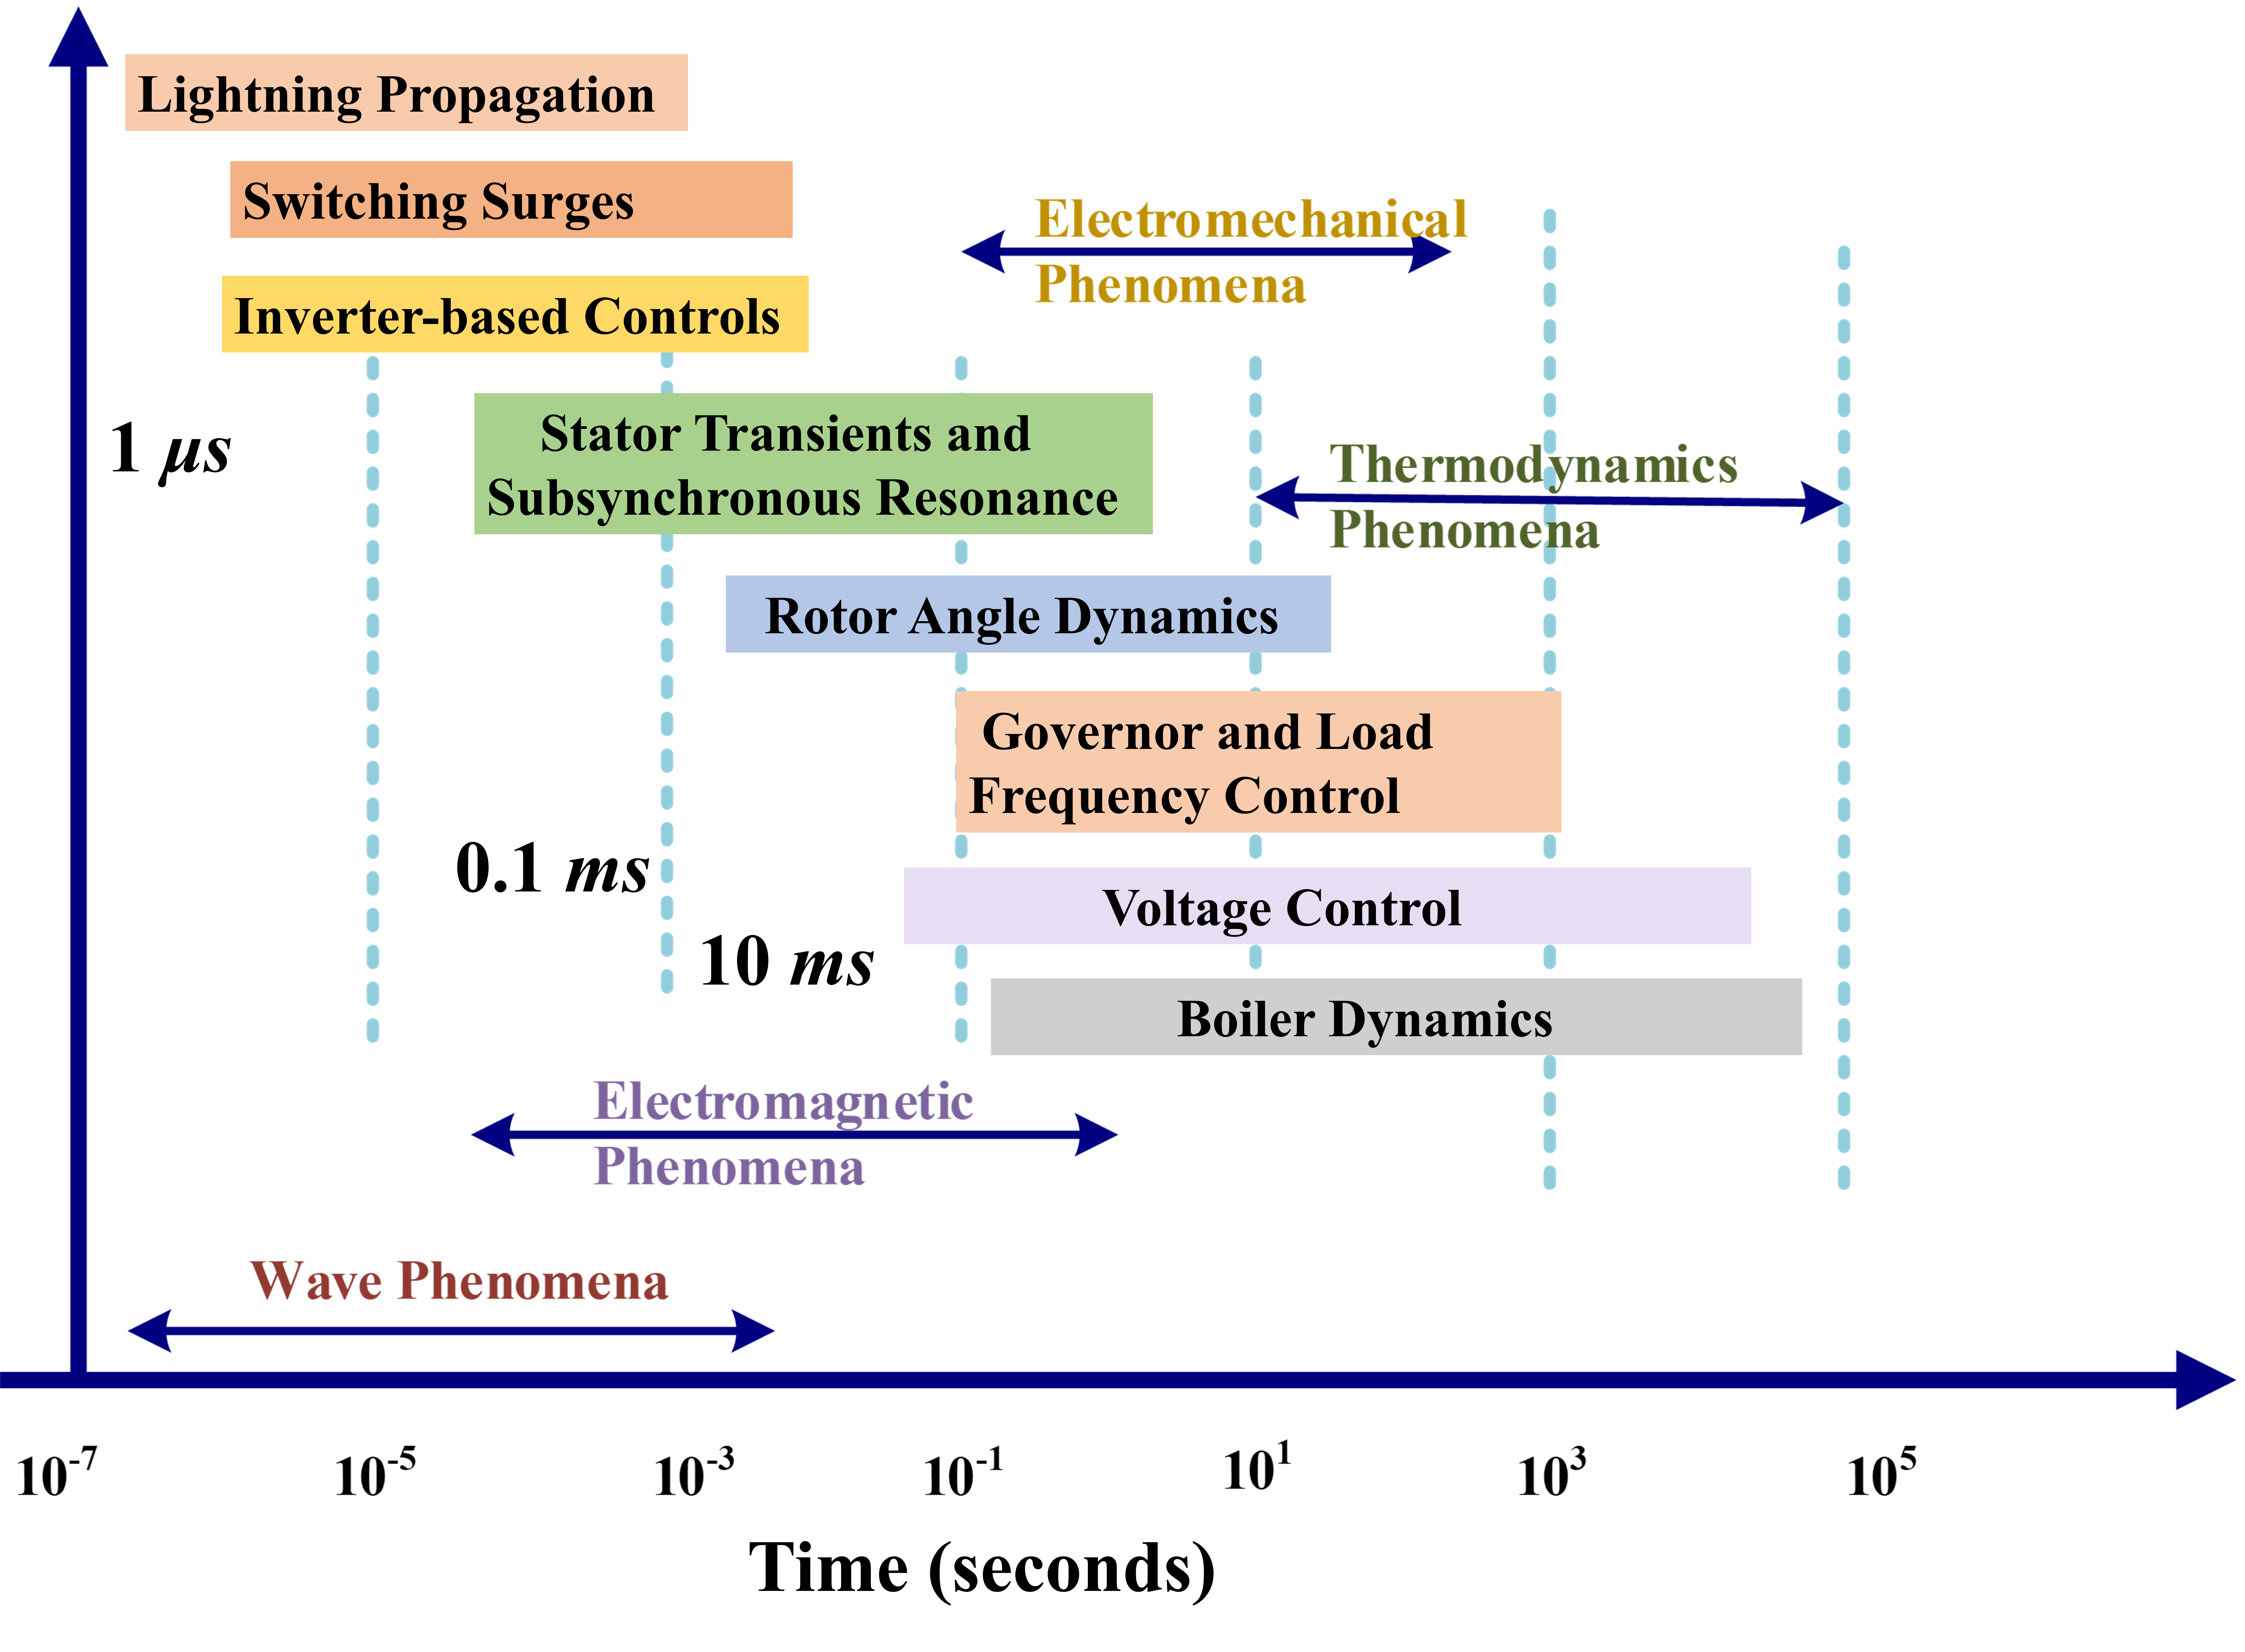
\includegraphics[width=3.3in]{Figures/singh25.png }}
\caption{Time Scales of Power System Dynamic Phenomena \cite{vega2020analysis}.}
\label{Dynamics.}
\end{figure}
\subsection{\textbf{Challenges in OWF Modeling}}
OWFs present a unique set of challenges for modeling due to complex environmental conditions and intricate interaction with the grid \cite{sajadi2018small, jia2023systems, veers2023grand}. OWF modeling faces challenges in capturing complex environmental conditions, integrating with the power grid, predicting energy output, and simulating large-scale wind farm dynamics. One primary challenge is accurately capturing the dynamic behavior of offshore wind turbines and their response to varying wind and ocean conditions. Offshore environments are characterized by high wind speeds, turbulent conditions, and significant wave interactions, which can impact turbine performance and structural integrity \cite{barthelmie2009modelling, otter2022review}. Furthermore, the distance from shore introduces logistical challenges for data collection and monitoring, necessitating sophisticated remote sensing techniques for model validation \cite{rinaldi2021current}.

Another critical challenge is the integration of OWFs into the main power grid while ensuring stability and reliability. OWFs often operate in close proximity to coastal regions with constrained grid infrastructure, which poses challenges for grid connection and power transmission. Modeling the interaction between OWFs and onshore grid systems requires an accurate representation of power electronics, grid dynamics, and control strategies to prevent instability and grid disturbances \cite{quester2019assessing, ali2021offshore}.

In addition, the variability and intermittency of wind resources present challenges for predicting power output and optimizing energy generation \cite{sulaeman2016wind}. Offshore wind conditions vary over time, ranging from seconds to seasons, making it challenging to forecast energy production and plan for grid integration accurately. Advanced stochastic modeling techniques and ensemble forecasting methods are needed to account for the inherent uncertainty in wind resources and improve the accuracy of energy yield predictions \cite{arenas2020stochastic, gong2024improving, hoang2023probabilistic}.

Moreover, the increasing scale and complexity of offshore wind projects introduce challenges for modeling and simulation \cite{yoro2021update}. Large-scale OWFs with hundreds of turbines require computationally intensive modeling approaches to simulate the interactions between individual turbines, wake effects, and overall farm performance \cite{wu2019key}. High-fidelity simulation tools, coupled with parallel computing techniques, are essential to capture the spatial and temporal dynamics of OWFs accurately \cite{zou2023modeling, nomandela2023modeling}. Addressing these challenges requires interdisciplinary research efforts and the development of advanced modeling techniques tailored to the unique characteristics of OWE systems.


\subsection{\textbf{Capturing Dynamics and Efficiency Trade-offs}}

Modeling wind turbine generation systems involves addressing complex challenges due to the dynamic nature of modern power systems. Accurate models are essential for representing transient events and high-frequency phenomena associated with power electronics, which are crucial to maintaining system stability and reliability \cite{zhang2016review}. However, capturing these intricate dynamics introduces computational challenges, requiring advanced modeling techniques to accurately reflect fast-changing behaviors without overwhelming computational resources \cite{karaagac2016offshore}.

These systems evolve rapidly, demanding simulations that can keep up with real-time changes while still providing meaningful results \cite{ganesh2021generic}. Ensuring computational efficiency is therefore critical to managing this complexity without compromising the accuracy required for reliable system operation. An additional challenge lies in selecting the appropriate level of model detail \cite{zou2023integrated}. The optimal level of abstraction depends on factors such as the specific phenomena under study, simulation time constraints, and the system's overall complexity. Although more detailed models can offer greater accuracy, they also increase computational demands. Striking the right balance between model precision and efficiency ensures that simulations remain practical, enabling insightful analysis while avoiding unnecessary computational overhead \cite{xia2023operation}.


\subsection{\textbf{Analytical Approaches: Time-Domain and Frequency-Domain Analysis}}
Modeling of OWF requires a comprehensive analytical approach that incorporates both time-domain and frequency-domain analysis to accurately represent dynamic behaviors, grid interactions, and energy conversion processes in varying operating conditions.\cite{deng2023review} provides a comparative analysis of time domain and frequency domain modeling techniques and their applications in stability analysis of HVDC OWFs.

Time-domain analysis is preferred for assessing component interactions and system stability, yet increasing complexity from power-electronic integration poses challenges. Frequency-domain methods are essential for understanding complex system dynamics and are particularly crucial in complex interactions that threaten stability. Frequency domain impedance modeling offers advantages such as wideband oscillation study, gray/black-box device modeling, combined impedance analysis, and multi-frequency instability study.

Table \ref{modeling comparison} gives a brief literature survey of various modeling techniques used for HVDC OWFs along with examples of models used in the economic domain. \cite{karaagac2016offshore} compares modeling accuracy and computational performance of modeling in multiple combinations of MMC and OWF models, including the Detailed Model (DM), Detailed Equivalent Circuit Model (DECM), Equivalent Switching Function Model (ESFM), and Average Value Model (AVM) and their limitations. \cite{castro2020dynamic} introduces a comprehensive RMS modeling framework for dynamic studies of Doubly Fed Induction Generator (DFIG)-based wind farms in multi-terminal VSC-HVDC grids, offering high fidelity and faster simulations than EMT solutions.

\cite{ji2019impedance} develops an offshore AC side impedance model for MMC-HVDC wind power integration, considering the effects of offshore / offshore stations and DC cables, to analyze the AC-DC system coupling and the impact of the DC system and controller on offshore AC impedance, overcoming deficiencies in harmonic resonance analysis. \cite{wang2022impedance} develops the impedance model and stability analysis for All-DC offshore Permanent Magnet Synchronous Generator
 (PMSG) wind farms, with simulations validating the model's effectiveness by reproducing time-domain oscillations. \cite{yu2021impedance} investigates the stability of DR-HVDC connected OWFs by developing and validating an impedance model in the dq frame and analyzes the impacts of the DC smoothing reactor and AC filter sizes of the DR-HVDC on system stability using PSCAD/EMTDC simulations. Fig. \ref{Timedomain.} and Fig. \ref{Frequencydomain.} provide a systematic categorization of modeling techniques in both the time and frequency domains applied in simulation studies of systems.

The accuracy of the model depends heavily on the level of detail incorporated into the representation. To ensure precision, non-linearities within the system are addressed through linearization techniques. This approach helps manage the complexities inherent in modeling, but it also highlights that the accuracy of stability predictions is intrinsically linked to the overall model accuracy. Therefore, maintaining high fidelity in model details is crucial for reliable stability analysis.

\begin{figure}[t]
\centerline{\includegraphics[width=3.5in]{Figures/singh26.png }}
\caption{Classification of Time Domain Simulation Methods.}
\label{Timedomain.}
\end{figure}


\begin{figure}[t]
\centerline{\includegraphics[width=3.5in]{Figures/singh27.png }}
\caption{Classification of Frequency Domain Simulation Methods.}
\label{Frequencydomain.}
\end{figure}

\begin{table*}[htbp]
\centering
\renewcommand{\arrayrulewidth}{1.1pt} % Increase border thickness
\arrayrulecolor{black}
\renewcommand{\arraystretch}{1.3} % Improve row height for readability
\small % Reduce font size slightly for compact formatting
\caption{Examples of HVDC Offshore Wind Farm Models}
\label{modeling comparison}
\begin{tabular}{|
p{1.8cm}|
p{5cm}|
p{7.4cm}|
p{1.4cm}|}
\hline
\textbf{Topology} & \textbf{Modeling Techniques} & \textbf{Key Points and Outcome} & \textbf{Reference} \\ 
\hline

 & 
MMC and OWF modeling DM, DECM, ESFM, AVM Time Domain Models & 
\begin{tabular}[]{@{}l@{}}$-$ Accuracy vs. computational efficiency for MMC and \\ \hspace{5pt} OWF models. \\ 
$-$ AVM (OWF) + DECM (MMC) boosts speed with \\ \hspace{5pt} minimal accuracy loss.\end{tabular} & 
\cite{karaagac2016offshore} \\  \hhline{|>{\arrayrulecolor{white}}-|>{\arrayrulecolor{black}}---} 

\multirow{4}{*}{\textbf{VSC-HVDC}} & Time Domain Modeling & 
\begin{tabular}[]{@{}l@{}}$-$ A comprehensive techno-economic comparison of \\ \hspace{5pt}  MT-HVDC OWFs.\\ 
$-$ A semidefinite programming model for optimal \\ \hspace{5pt} economic operation in MT-HVDC systems.\end{tabular} & 
\cite{raza2020multi, zhou2019optimal} \\  \hhline{|>{\arrayrulecolor{white}}-|>{\arrayrulecolor{black}}---} 

& RMS modeling & 
\begin{tabular}[]{@{}l@{}}$-$ Introduction of RMS model for MTAC/DC grids for \\ \hspace{5pt}  VSC-DFIG WFs. \\ 
$-$ Flexible and numerically efficient.\end{tabular} & 
\cite{castro2020dynamic} \\  \hhline{|>{\arrayrulecolor{white}}-|>{\arrayrulecolor{black}}---} 

& AC Side Impedance modeling & 
\begin{tabular}[]{@{}l@{}}$-$ AC side impedance model for MMC-HVDC wind \\ \hspace{5pt} integration. \\ 
$-$ Analysis with different DC system configurations. \\ 
$-$ Influence of dual closed-loop control indicated.\end{tabular} & 
\cite{ji2019impedance} \\ 
\hline 

\textbf{All-DC} & 
Impedance modeling & 
\begin{tabular}[]{@{}l@{}}$-$ Harmonic linearization for impedance modeling of \\ 
\hspace{5pt}All-DC  WF  with PMSG and LCC-inverter. \\ 
$-$ Verification through simulation and oscillation analysis.\end{tabular} & 
\cite{wang2022impedance} \\ 
\hline

\textbf{DR-HVDC} & 
Impedance Model of Connected OWF & 
\begin{tabular}[]{@{}l@{}}$-$ Investigates DR-HVDC connected OWF stability. \\ 
$-$ Impedance model in dq frame developed, validated \\ 
\hspace{5pt}vs. EMT simulations. \\ 
$-$ DR-HVDC's DC smoothing reactor and AC filter sizes \\ 
\hspace{5pt}impact system stability.\end{tabular} & 
\cite{yu2021impedance} \\ 
\hline

\end{tabular}
\end{table*}



Several research gaps need to be addressed to improve modeling techniques. One significant area is understanding the impact of frequency coupling on system stability. Additionally, effective addressing non-linearities such as PWM and limiters remains a challenge. There is also a need to develop independent models that can adapt to changing conditions within the system. Furthermore, analyzing the interactions between sources and loads and the complexities of impedance networks presents ongoing challenges that require innovative solutions.

\subsection{\textbf{Research Gaps and Areas for Exploration}}
Electrical modeling is a foundational aspect of designing and operating large-scale HVDC OWFs. Although significant progress has been made in the development of various modeling techniques, ongoing research is essential to address existing gaps and explore new areas of innovation. By advancing electrical modeling techniques, we can ensure offshore wind power's efficient and reliable integration into the global energy grid, contributing to a sustainable energy future.
Addressing these challenges reveals several research gaps and areas demanding further exploration in wind turbine generation modeling:

\textbf{Novel Modeling Methods:} Advanced techniques, such as Digital Twin models \cite{haghshenas2023predictive}, data-driven modeling \cite{wang2021mixed}, and multi-scale modeling \cite{marinescu2022dynamic}; enable real-time monitoring and predictive analysis \cite{nguyen2023real}. These models enhance system performance by providing detailed insights into both component-level behavior and overall system dynamics, facilitating proactive decision-making and optimization. As the complexity of wind power systems continues to increase, combining these advanced techniques with existing methods will enable more efficient, reliable, and scalable integration of OWE into the global grid.

\textbf{Efficient Representation of Fast Dynamics:} Capturing the rapid dynamics of power electronics remains a challenge due to the high computational demand of such simulations. Advanced techniques such as reduced-order models can help simplify the representation of high-frequency switching without sacrificing accuracy \cite{subedi2021review}. Such models enable grid operators to simulate fault scenarios quickly and develop appropriate control strategies to ensure system stability. %Research endeavors should enhance modeling techniques that efficiently capture high-speed dynamics within power electronics without compromising computational feasibility.

\textbf{Co-simulation Techniques:} Co-simulation offers a powerful method to integrate different models to capture various aspects of OWF operations \cite{da2023modeling}. By combining phasor-based grid models with detailed models of converter-interfaced devices, researchers can study interactions between the grid and converters under complex scenarios \cite{raab2022hybrid}. This holistic approach is crucial for identifying potential risks and designing robust control schemes for hybrid AC/DC systems.%Exploring co-simulation methods, and integrating power grid models (e.g., phasor models) with converter-interfaced devices, such as power electronics, aids in comprehensive studies encompassing diverse aspects like stability, protection, and control in CIG integration scenarios.

\textbf{Full Phasor Model (PM) for CIG Integration:} Implementing full PM for studies involving CIG enables a more comprehensive analysis of system stability, protection, and control \cite{lacerda2022phasor}. Full PM models offer a valuable framework for designing control strategies, ensuring reliable fault ride-through capabilities, and maintaining grid stability by accurately representing the voltage and current phasors over time. %Investigating the implementation of full Phasor Model (PM) models in studies involving CIG integration allows for a more comprehensive understanding of stability, protection, and control aspects within the power system.

\textbf{Integrated Economic Stochastic Optimal Control:}

HVDC OWF poses a unique opportunity for economic models of stochastic optimal control and operational bidding behaviors to start \cite{rinaldi2021incorporating,sun2019vsc,rabiee2014information}. HVDC architectures can potentially provide more parameters for OWF operators, including control over line losses, faster interaction with the grid, and potential for black start capability \cite{sakamuri2019black}. As such, work should be done to advance the stochastic optimal control literature to optimize both economic and engineering parameters. 

This requires significant advancement in dynamic models that consider large state spaces and choice sets to optimize bidding in both financial and physical markets with power and ancillary services markets. The problem of simultaneously bidding in the day-ahead, inter-day, real-time, and ancillary services markets proves particularly difficult under these, particularly when OWF is colocated with Energy Storage System \cite{shahmohammadi2018market,cciccek2021optimal}. Recent developments in reinforcement learning algorithms may have potential in this domain \cite{wu2022strategic}.

\section{\textbf{Ongoing Research and Future Scope}}

As offshore wind approaches technological maturity and market saturation, research continues to explore its role in the future energy grid. Four key factors—{connection topology, converter design, technical modeling, and economic considerations}—are essential in shaping decisions regarding offshore wind adoption.

\textbf{{Challenges and Key Research Areas}}
\begin{itemize}
\item {Grid Architecture}
\begin{itemize}
\item Scalability, complexity, reliability, suitability, and cost are crucial in selecting grid configurations. Effective {load management techniques} are required to address the challenges of integrating offshore systems with existing onshore grids.
\end{itemize}

\item {Converter Technologies}
\begin{itemize}
    \item Although earlier VSC systems are well researched, emerging technologies, such as medium-frequency systems, transformer-embedded HVDC, and {series DC grids}—show promise but need further exploration.
    \item Solid-state transformers in HVDC grids and {DC-DC converter prototypes} must be investigated to improve cost, reliability, and performance.
\end{itemize}

\item{Fault Management and Intelligent Protection}
\begin{itemize}
\item Reliable and fast fault detection in HVDC offshore systems remains a significant challenge due to weak fault signatures, measurement noise, and the fast-changing dynamics of converter-based grids. There is a growing need for advanced protection schemes that are adaptive, noise-resilient, and capable of operating under varying system conditions in real time.
\end{itemize}

\item {Modeling and Computational Advances}
\begin{itemize}
\item {Modeling Techniques:} Future research should focus on improving the capabilities of dynamics, accuracy, and {co-simulation} capabilities by integrating phasor models with CIG systems for better stability and control.

\item {Algorithm Design:} Computational innovations are required to simulate complex models efficiently and improve overall system operations.
\end{itemize}

\item {{Economic and Market Integration}}
\begin{itemize}
\item {Holistic Market Integration:} Offshore wind engineering decisions affect the broader energy market, influencing {long-term costs, revenues, and market equilibrium}. Transmission infrastructure impacts {investment decisions} and {market entry/exit dynamics}, requiring comprehensive study.

\item {Interest Rates and Market Design:} As rising interest rates challenge project viability, research into new market models—such as comparing the {UK and German funding frameworks}—is needed to address these risks.
\end{itemize}

\item {{Reliability and Social Costs}}

\begin{itemize}
\item {Reliability Trade-offs:} Future work should explore the cost-benefit trade-offs between enhanced reliability through technical solutions and the associated economic impacts. Rather than focusing on isolated components, a system-wide approach to reliability is essential.

\item {Social Costs:} Models must incorporate social costs—an aspect often overlooked—as renewable energy displaces fossil fuels.
\end{itemize}

\item {{Bridging Technical and Economic Analysis:}}
Future research must integrate {technical and economic insights} by combining architectural choices with long-term impacts on {LCOE, construction timelines}, and system costs. This holistic approach will help align technical feasibility with economic sustainability, ensuring offshore wind development remains viable and resilient.
\end{itemize}


\section{\textbf{Conclusions}}

This review evaluates HVDC technology integration in OWFs, examining economic considerations, connection topologies, converter designs, and technical modeling to optimize the performance and efficiency of collection and transmission systems. It explores the {techno-economic aspects of HVDC OWFs}, focusing on collection and transmission costs, system reliability, and architecture. It analyzes both LCOE and LACE, along with breakeven distances between HVDC and HVAC systems based on costs and performance. The study highlights how improving HVDC reliability is essential for economic viability and how engineering advancements can address these challenges. The paper reviews global wind farm installation capacity and assesses various collection and transmission architectures, paying particular attention to emerging designs such as {MTDC grids} and {All-DC systems}, which offer improved scalability, efficiency and reliability with reduced footprint for large OWFs.

Furthermore, the article examines the topologies of the power converters, focusing on the role of {AC/DC and DC/DC converters}. A comparison between LCC and VSC is presented, along with an exploration of emerging technologies such as MMC and AAMC. While VSCs are recognized as the preferred option for medium-voltage DC collection, MMCs demonstrate significant advantages for offshore wind transmission. Additionally, DC/DC converters offer key benefits in terms of reducing system footprint and optimizing costs, as they enable efficient voltage conversion, eliminate the need for bulky offshore transformers, and enhance integration between DC collection grids and HVDC transmission systems.


Modeling offshore wind systems present significant challenges due to complex environmental conditions and the highly variable output of wind farms. The paper explores analytical methods in both the time and frequency domains to maintain the stability of the grid as the penetration of offshore wind increases.
The review concludes by outlining key future research directions, including the need to improve system scalability, reduce architectural complexity, and develop next-generation converter technologies tailored with advanced and real-time fault detection and management techniques for offshore applications. It also emphasizes the importance of interdisciplinary collaboration to ensure that technical advancements align with economic and regulatory realities. 

As OWFs expand in scale and are deployed farther from shore, grid operators will increasingly rely on complex HVDC architectures for long-distance transmission. This transition demands a clear understanding of HVDC system capabilities, limitations, and their impact on overall grid stability. By applying the insights presented in this review—spanning techno-economic analysis, system design, and modeling approaches—grid planners and operators can make informed decisions that enhance reliability, reduce costs, and support the safe integration of large-scale offshore wind energy. Ultimately, this article offers a comprehensive foundation for building resilient, efficient, and economically viable HVDC-based offshore power systems.


\bibliographystyle{ieeetr}
\bibliography{References}

\phantomsection
\vspace{-1cm}
\begin{IEEEbiography}[{
\includegraphics[width=1in,height=1.25in,clip,keepaspectratio]{Pic_author/singd.png}}]{Deepi Singh} received the bachelor's degree in electrical engineering
from Muzaffarpur Institute of Technology, Muzaffarpur, Bihar, India, and the master's degree in power and controls from the Indian Institute of Information Technology, Jabalpur, Madhya Pradesh, India, in 2017. She is currently working toward her Ph.D. degree in electrical engineering at Stony Brook University, Stony Brook, New York, USA. She has three years of teaching and research experience as an Assistant Professor at the Government Engineering College, Bilaspur, Chhattisgarh, India, under the Technical Education Quality Improvement Project III of the World Bank. She has recently completed her research internship as a Power and Control Engineer at Mitsubishi Electrical Research Lab (MERL). Her research interests include the domain of distributed energy resources and their impeccable grid integration, advanced control methodologies, the augmentation of microgrid resiliency, and the intricate realm of real-time power system monitoring.
\end{IEEEbiography}
\vspace{-1cm}
\begin{IEEEbiography}[{
\includegraphics[width=1in,height=1.25in,clip,keepaspectratio]{Pic_author/golde.png}}]{Dana Golden} received B.S. and M.S. degrees in economics from the Georgia Institute of Technology in Atlanta, in 2018. She also received an M.S. degree in analytics in 2022. From 2019 to 2021, she worked as an Agricultural Economist for the USDA Economic Research Service. She interned as an Industry Analyst at the Federal Energy Regulatory Commission in the Summer of 2022. She also worked as a Data Scientist for the Treasury and an economist for the USDA Economic Research Service in 2023. Since 2021, She has been a PhD Student in economics at Stony Brook University. Her research interests focus mainly on energy markets, machine learning, and empirical industrial organization. Ms. Golden was a recipient of the Stony Brook Economics Diversity Fellowship in 2021 and the Bias NRT Fellowship in 2023.
\end{IEEEbiography}
\vspace{-1cm}
\begin{IEEEbiography}[{
\includegraphics[width=1in,height=1.25in,clip,keepaspectratio]{Pic_author/bhans.png}}]{Gaurav Bhansali} earned his degree in Electrical Engineering from Jai Narain Vyas University (JNVU), in 2012 and did his Masters in Power Systems from Malaviya National Institute of Technology (MNIT), Jaipur, India in 2014. Currently, he is pursuing his Ph.D. in Electrical Engineering from Stony Brook University, New York, USA. His research interest includes the development of DC-DC and AC-DC power electronic converters utilizing wide band gap (WBG) devices for renewable energy and hydrogen generation applications. His work emphasizes control and optimization strategies for Hybrid Energy Grid networks. Before joining PhD, he worked extensively in the power sector, focusing on the design and execution of power distribution grid networks for smart cities and power trading for the distribution business. 
\end{IEEEbiography}
\vspace{1.2cm}
\begin{IEEEbiography}[{
\includegraphics[width=1in,height=1.25in,clip,keepaspectratio]{Pic_author/anwar.png}}]{Ali Anwar} received the B.S. degree in Electrical Engineering from GIK Institute, Pakistan, in 2010, and the M.E. degree in Electrical Engineering from RMIT University, Melbourne, Australia, in 2016. He is currently pursuing his Ph.D. degree in Electrical Engineering with the Spellman High Voltage Power Electronics Laboratory, Department of Electrical and Computer Engineering, Stony Brook University, New York, USA. 
His research interests include power electronic converter design, analyzing and mitigating electromagnetic interference (EMI) in wide-bandgap (WBG) device-based power converters, partial discharge phenomena, and reflected wave modeling in motor drives.
\end{IEEEbiography}
\vspace{-1cm}
\begin{IEEEbiography}[{
\includegraphics[width=1in,height=1.25in,clip,keepaspectratio]{Pic_author/sings.png}}]{Shreepooja Singh} received the B.Tech. degree in Electrical and Electronics Engineering from SRM Institute of Science and Technology, India, and the M.Tech. degree in Power Electronics and Systems from Delhi Technological University, India. She is currently pursuing her Ph.D. degree in Power Electronics with the Spellman High Voltage Power Electronics Laboratory, Department of Electrical and Computer Engineering, Stony Brook University, New York, USA.
Her research interests include the integration of power electronic converters and advanced battery management systems for renewable energy applications, as well as enhancing the reliability and resiliency of microgrids to improve the efficiency and sustainability of future energy networks.
\end{IEEEbiography}
\vspace{-1.0cm}
\begin{IEEEbiography}[{
\includegraphics[width=1in,height=1.25in,clip,keepaspectratio]{Pic_author/luofa.png}}]{Fang Luo} received the bachelor's and Ph.D. degrees in power electronics from the Huazhong University of Science and Technology, Wuhan, China, and jointly from Virginia Tech,
Blacksburg, VA, USA, in 2003 and 2010, respectively. He was an Assistant Professor with the Electrical Engineering Department, University of Arkansas, Fayetteville, AR, USA, from 2017 to 2020, and a Research Assistant Professor with The Ohio State University, Columbus, OH, USA, from 2014 to 2017. He was a Visiting Ph.D. student, from 2007 to 2010, and then a Postdoctoral Researcher, from 2010 to 2014, with Virginia Tech, Blacksburg, VA, USA. He is currently an Empire Innovation Associate Professor and the Director of the Spellman High Voltage Laboratory, Stony Brook University (SUNY Stony Brook), Stony Brook, NY, USA, with his background in power electronics. His research interests include high power density converter design, high-density electromagnetic interference filter design and integration, and power module
packaging/integration for wide bandgap devices. Dr. Luo is also a Member of American Institute of Aeronautics and Astronautics and American Society of Mechanical Engineers. He was the recipient of the NSF CAREER Award.
\end{IEEEbiography}
\vspace{-1.0cm}
\begin{IEEEbiography}[{
\includegraphics[width=1in,height=1.25in,clip,keepaspectratio]{Pic_author/zhou.png}}]{Yiyi Zhou} received a BA in Finance from University of International Business and Economics in Beijing, China. She then received an MA in economics from Peking University in Peking, China followed by a PhD in economics from from the University of Virginia in Charlottesville, Virginia. Since 2012, she has served as a Professor in the Departments of Economics and Business at Stony Brook University. Her publications include "The Market for Electric Vehicles: Indirect Network Effects and Policy Impacts" and "An Equilibrium Search Model of Inventory Management". Her research interests focus on Industrial Organization, Environmental Economics, and Health Economics. Dr. Zhou recieved the Snavely Dissertation Prize from the University of Virginia in 2012 and the Summer Grant of the NET Institute in 2015.
\end{IEEEbiography}

\EOD

\end{document}
